% ============================================================================ %
%
%           Šablona bakalářské/diplomové práce
%
% Autor:    Ing. Jozef Říha (2006-05-04), od té doby šablonu udržuje
%           Ing. Pavel Tomášek, Ph.D. (tomasek@utb.cz)
%
% Verze:    2021-05-04
%
% Kódování: UTF-8 (kontrolní řetězec: žluťoučký kůň úpěl ďábelšké ódy)
%
% Sazba:    pdflatex prace.tex && pdflatex prace.tex
%           (nutné dvakrát pro korektní vložení citací a jiných referencí),
%           v případě umístění literatury do externího bib souboru je třeba volat
%           pdflatex prace.tex && bibtex prace && pdflatex prace.tex && pdflatex prace.tex
%
% Tip:      Ve správně vysázeném českém textu by na konci řádku neměla zůstant
%           samotná jednopísmenná předložka či spojka. Na takové místo se vkládá
%           nezalomitelná mezera pomocí symbolu ~. Existuje program, který umí
%           zpracovat celý TeX dokument najednou podle českých konvencí:
%           http://petr.olsak.net/ftp/olsak/vlna/
%
% Pozor:    Vzhledem k požadovanému standardu PDF/A nesmí vložené obrázky 
%           obsahovat alfa kanál (průhlednost).
%
% ============================================================================ %


\documentclass[a4paper,12pt]{article}

% Definice vzhledu a nastavení se načítá z následujícího souboru (netřeba editovat)
% ============================================================================ %
% Tento dokument není zpravidla třeba editovat,
% obsahuje nastavení balíčků, vzhledu, stylů.
%
% Kódování: UTF-8 (žluťoučký kůň úpěl ďábelšké ódy)
% ============================================================================ %


% ============================================================================ %
% BALÍČKY

%\usepackage[czech,english]{babel} % volba při kompilaci latexem (vyžaduje texlive-lang), zakomentovano, nastavovanu prikazem \nastavjazyk
\usepackage[T1]{fontenc}% definice vnitřního kódování
\usepackage[utf8x]{inputenc} % slouží pro definici kódování (při problémech zkusit zaměnit utf8x za utf8)
\usepackage{color}		% umožňuje použití barev
\usepackage{graphicx}	% rozšíření práce s grafikou
\usepackage{amsmath}	% balíček pro pokročilejší matematiku
\usepackage{fancyhdr}	% detailnější nastavení záhlaví a zápatí
\usepackage{tocloft}	% umožňuje pohodlné nastavení vzhledu obsahu, seznamu tabulek či obrázků
\usepackage{textcase}	% změna VeLiKoStI PíSmA
\usepackage{ifthen} 	% balíček umožňující skladby if, then -- využijeme při definici nadpisů
\usepackage{setspace}	% balíček umožňující nastavit řádkování na 1, 1.5, 2
\usepackage{ccaption}	% vylepšení práce s popisky obrázků či tabulek
\usepackage{sectsty}	% pro nastavení vzhledu nadpisů
\usepackage[srcstyle=leftnumhang,linenumbersep={\ }]{examplep} % pokročilejší sazba programového kódu
\usepackage{url}		% balíček pro vysázení internetové adresy stylem verbatim s vylepšeným řádkovým zlomem
\usepackage{afterpage}
%\usepackage{layout}	% zobrazí nastavení tiskového zrcadla (příkaz \layout)
%\usepackage{times}		% balíček pro použití fontu times
%\usepackage{verbatim}	% vysází text bez formátování, tak jak je zapsán v souboru
%\usepackage{indentfirst} % definuje odsazení prvního řádku odstavce
%\usepackage{makeidx}	% vytvoří rejstřík
\usepackage[pdftex,pdfa,hidelinks,breaklinks]{hyperref}	% vytváří křížové odkazy
%\usepackage{multicol}	% vícesloupcová sazba
%\usepackage{flafter}	% zajistí, aby se plovoucí objekty objevovali až za jejich umístěním v textu
\usepackage{chngcntr}	% Umožňuje změnu nastavení číslování obrázků, tabulek i rovnic
\usepackage{etoolbox}	% Tool-box for LaTeX programmers
\usepackage[labelsep=space,tableposition=bottom,justification=centering]{caption} % Přenastavení popisků u figur a tabulek
\usepackage{xmpincl}	% Pro aplikaci standardu PDF/A
\usepackage{hyperxmp}	% Pro aplikaci standardu PDF/A

\usepackage{svg}
\usepackage{dirtree}
\usepackage{float}
\usepackage{pdfpages}


%\usepackage{hhline}
\usepackage{multirow}	% vícesloupcová sazba

%\pdfminorversion=4
%\pdfobjcompresslevel=0

%language definitions
\usepackage{listings}
\definecolor{delim_json}{RGB}{20,105,176}
\definecolor{numb_json}{RGB}{106, 109, 32}
\definecolor{string_json}{rgb}{0.64,0.08,0.08}
\lstdefinelanguage{json}{
  frame=single,
  rulecolor=\color{black},
  showspaces=false,
  showtabs=false,
  breaklines=true,
  basicstyle=\ttfamily,
  morestring=[b]",
  stringstyle=\color{string_json},
  literate=
   *{:}{{{\color{delim_json}{:}}}}{1}
   {,}{{{\color{delim_json}{,}}}}{1}
   {\{}{{{\color{delim_json}{\{}}}}{1}
   {\}}{{{\color{delim_json}{\}}}}}{1}
   {[}{{{\color{delim_json}{[}}}}{1}
   {]}{{{\color{delim_json}{]}}}}{1},
  morekeywords={true,false,null},
  keywordstyle=\color{numb_json},
}


% ---------------------------------------------------------------------------- %

% NASTAVENÍ TISKOVÉHO ZRCADLA

\newcommand{\valueTextHeight}{242mm}	% výška tiskového zrcadla
\newcommand{\valueTextWidth}{155mm}	% šířka tiskového zrcadla
\newcommand{\valueVOffset}{-1.61cm}	% vertikální posunutí tiskového zrcadla
\newcommand{\valueSideMargin}{0.96cm}	% levý okraj
\newcommand{\valueHeadHeight}{0.6cm}	% záhlaví
\newcommand{\valueHeadSep}{1cm}	% záhlaví

\textheight=\valueTextHeight
\textwidth=\valueTextWidth
\voffset=\valueVOffset
%\voffset=-1in
%\topmargin=-2.9cm

\oddsidemargin=\valueSideMargin
\evensidemargin=\valueSideMargin

\headheight=\valueHeadHeight
\headsep=\valueHeadSep

% nastavení zápatí
\footskip=1ex
\cfoot{}
% "vypnout" poznámky na okrajích
\marginparpush=0mm
\marginparwidth=0mm
\marginparsep=0mm

\pagestyle{fancy}

% Nastavení obalujících okrajů okolo popisků figur a tabulek
\captionsetup[figure]{aboveskip=5pt}
\captionsetup[figure]{belowskip=0pt}
\captionsetup[table]{aboveskip=0pt}
\captionsetup[table]{belowskip=5pt}


% ============================================================================ %
% NASTAVENÍ PÍSMA, ODSTAVCE, ROVNIC, POZNÁMEK

\parindent=0em				% velikost odstavcové zarážky na nulu
\def\thefootnote{\arabic{footnote})}	% poznámka pod čarou se závorkou
\onehalfspacing % nastavím řádkování tímto způsobem nebo \renewcommand{\baselinestretch}{1.5} ??
\setlength{\parskip}{3pt}		% vertikální mezera mezi nadpisy
%\def\label#1{{\sf ! #1 ! }}		% možnost zobrazení všech \label{}


% ============================================================================ %
% NASTAVENÍ ČÍTAČŮ

\setcounter{tocdepth}{3} % do obsahu se ukládají pouze první dvě úrovně kapitol


% ============================================================================ %
% PDF/A STANDARD

% http://www.mathstat.dal.ca/~selinger/pdfa/
% https://blog.zhaw.ch/icclab/creating-pdfa-documents-for-long-term-archiving/
% http://support.river-valley.com/wiki/index.php?title=Generating_PDF/A_compliant_PDFs_from_pdftex

% Prerequisites: pdflatex, hyperref, xmpincl
% pdfTeX at least in version 1.40.15 (in Linux add repository ppa:jonathonf/texlive, update and upgrade texlive-full)
%
% Validator: http://pdfa.k.utb.cz:8080/ https://www.pdf-online.com/osa/validate.aspx

% \convertDate converts D:20080419103507+02'00' to 2008-04-19T10:35:07+02:00
\def\convertDate{%
	\getYear
}
{\catcode`\D=12
 \gdef\getYear D:#1#2#3#4{\edef\xYear{#1#2#3#4}\getMonth}
}
\def\getMonth#1#2{\edef\xMonth{#1#2}\getDay}
\def\getDay#1#2{\edef\xDay{#1#2}\getHour}
\def\getHour#1#2{\edef\xHour{#1#2}\getMin}
\def\getMin#1#2{\edef\xMin{#1#2}\getSec}
\def\getSec#1#2{\edef\xSec{#1#2}\getTZh}
\def\getTZh +#1#2{\edef\xTZh{#1#2}\getTZm}
\def\getTZm '#1#2'{%
	\edef\xTZm{#1#2}%
	\edef\convDate{\xYear-\xMonth-\xDay T\xHour:\xMin:\xSec+\xTZh:\xTZm}%
}
\expandafter\convertDate\pdfcreationdate

\pdfminorversion 4

\immediate\pdfobj stream attr{/N 3} file{graphics/sRGBIEC1966-2.1.icm}
\pdfcatalog{%
	/OutputIntents [ <<
	/Type /OutputIntent
	/S/GTS_PDFA1
	/DestOutputProfile \the\pdflastobj\space 0 R
	/OutputConditionIdentifier (sRGB IEC61966-2.1)
	/Info(sRGB IEC61966-2.1)
 >> ]
}

\providecommand{\xmpOrg}{Tomas Bata University in Zlín, Czech Republic}
\providecommand{\xmpProducer}{}
\providecommand{\xmpDoi}{}
\providecommand{\xmpJournalnumber}{}
\providecommand{\xmpVolume}{}
\providecommand{\xmpIssue}{}
\providecommand{\xmpCoverDisplayDate}{}
\providecommand{\xmpCoverDate}{}
\providecommand{\xmpJournaltitle}{}
\providecommand{\xmpFirstpage}{}
\providecommand{\xmpLastpage}{}
\providecommand{\xmpAuthoritativeDomain}{}
\providecommand{\xmpCreatorTool}{}%pdfTeX

\newcommand{\aplikujpdfa}{
	\ifczech
		\providecommand{\xmpTitle}{\nazevcz}
		\providecommand{\xmpAuthor}{\autor}
		\providecommand{\xmpKeywords}{\klicovaslovacz}
		\hypersetup{
			pdftitle={\nazevcz},
			pdfauthor={\autor},
			pdfsubject={\abstraktcz},
			pdfkeywords={\klicovaslovacz},
			%pdfproducer={pdfTeX-1.40.20},
			pdflang=la,
			pdfapart=3,
			pdfaconformance=B,
			pdflang={cz}
		}
	\else \ifenglish
		\providecommand{\xmpTitle}{\nazeven}
		\providecommand{\xmpAuthor}{\autor}
		\providecommand{\xmpKeywords}{\klicovaslovaen}
		\hypersetup{
			pdftitle={\nazeven},
			pdfauthor={\autor},
			pdfsubject={\abstrakten},
			pdfkeywords={\klicovaslovaen},
			%pdfproducer={pdfTeX-1.40.20},
			pdflang=la,
			pdfapart=3,
			pdfaconformance=B,
			pdflang={en}
		}
	\fi \fi
	
	\makeatletter
	\includexmp{tex/pdfa-1b}
	\makeatother
}


% ============================================================================ %
% UŽIVATELSKÉ STYLY

% Styl nn = nečíslovaný nadpis (je vysázený v obsahu)
\def\nn#1{\clearpage\phantomsection\addcontentsline{toc}{section}{#1}\section*{\MakeTextUppercase{#1}}}

% Styl nm = nečíslovaný nadpis (není vysázený v obsahu)
\def\nm#1{\clearpage\section*{\MakeTextUppercase{#1}}}

% Styl ns = nečíslovaný nadpis na stejné stránce (není vysázený v obsahu)
\def\nns#1{\section*{\MakeTextUppercase{#1}}}

% Styl n{ur}{nadp} pro nadpisy, kde ur je číslo úrovně a nadp je text nadpisu
\def\n#1#2{
	
	\ifthenelse{#1=1}{
		\sectionfont{\normalsize\MakeUppercase}
		\clearpage\section{#2}
		\sectionfont{\normalsize}
		}{
		\ifthenelse{#1=2}{\subsection{#2}}{
			\ifthenelse{#1=3}{\subsubsection{#2}}{\paragraph{\itshape\bfseries{#2}}
}}}}

% Styl pro obrázky
% \obr{popisek}{label}{rozměr (0.0 - 1.0)}{soubor}
\def\obr#1#2#3#4{
	\begin{figure}[h]
		\centering
		\includegraphics[width=#3\linewidth]{#4}
		%\captionwidth{#3\linewidth}
		%\changecaptionwidth
		\captionsetup{width=#3\linewidth}
		\caption{#1}
		\label{#2}
	\end{figure}
}

% Styl pro tabulky
% \tab{popisek}{label}{rozměr (0.0 - 1.0)}{definice sloupců}{obsah} 
\def\tab#1#2#3#4#5{
	\begin{table}[h]
		%\captionwidth{#3\linewidth}
		%\changecaptionwidth
		\captionsetup{width=#3\linewidth}
		\caption{#1}
		\label{#2}
		\centering
		\begin{tabular}{#4}
			#5
		\end{tabular}
	\end{table}
}

% Styl pro tabulky v příloze
% \tabpri{popisek}{definice sloupců}{data tabulky}
\def\tabpri#1#2#3{
	\begin{table}[h]
	\begin{center}
	#1
	\end{center}
	\begin{center}
	\begin{tabular}{#2}
	#3
	\end{tabular}
	\end{center}
	\end{table}
}
	
% Styl pro tabulky z MS Excelu exportované do EPS
% \extab{popisek}{rozměr (0.0 - 1.0)}{soubor}
\def\extab#1#2#3{
	\begin{table}
	%\captionwidth{#2\linewidth}
	%\changecaptionwidth
	\captionsetup{width=#2\linewidth}
	\caption{#1}
	\begin{center}
	\includegraphics[width=#2\linewidth]{#3}
	\end{center}
	\end{table}
}

% Styl pro rovnice
% \rov[klíčové slovo]{rovnice}
\newcommand{\rov}[2][chybejici rovnice]{
	\begin{equation}
	#2
	\label{#1}
	\end{equation}
}
	
% Příkaz pro vysázení seznamu obrázků
\def\seznamobr{
	\clearpage
	\phantomsection
	\ifczech
		\addcontentsline{toc}{section}{Seznam obrázků}
	\else \ifenglish
		\addcontentsline{toc}{section}{List of Figures}
	\fi \fi
	\listoffigures
	\clearpage
}

% Příkaz pro vysázení seznamu tabulek
\def\seznamtab{
	\clearpage
	\phantomsection
	\ifczech
		\addcontentsline{toc}{section}{Seznam tabulek}
	\else \ifenglish
		\addcontentsline{toc}{section}{List of Tables}
	\fi \fi
	\listoftables
	\clearpage
}

\newcommand{\OdsazovaniOdstavcuStart}[0]{
	\ifenglish
		\setlength{\parskip}{5mm} % English indentation of paragraphs
	\else \ifczech
		\setlength{\parindent}{5mm} % Czech indentation of paragraphs
	\fi \fi
}

\newcommand{\OdsazovaniOdstavcuStop}[0]{
	\ifenglish
		\setlength{\parskip}{0mm} % English indentation of paragraphs
	\else \ifczech
		\setlength{\parindent}{0mm} % Czech indentation of paragraphs
	\fi \fi
}

% Příkaz pro vysázení seznamu literatury
\newcommand{\seznamlit}[1]{
	\clearpage
	\phantomsection
	\ifczech
		\addcontentsline{toc}{section}{Seznam použité literatury}
	\else \ifenglish
		\addcontentsline{toc}{section}{References}
	\fi \fi
	\begin{thebibliography}{99}
	#1
	\end{thebibliography}
}

\newcommand{\seznamlitbib}{
	\bibliographystyle{\ifenglish tex/czechiso-en\else\ifczech tex/czechiso-cz\fi\fi} % Respects the norm of ČSN ISO 690
	\newpage
	\clearpage
	%\cleardoublepage
	\phantomsection
	\addcontentsline{toc}{section}{\ifenglish References \else \ifczech Seznam použité literatury \fi \fi}
	\bibliography{tex/literatura}
}

% Příkaz pro přípravu seznamu použitých zkratek a symbolů
\newcommand{\seznamzkr}{
	\ifczech
		\nn{Seznam použitých symbolů a zkratek}
	\else \ifenglish
		\nn{List of Abbreviations}
	\fi \fi
}

% Příkaz \cast jako alternativa k \part
\def\cast#1{
	\clearpage
	\part{#1}
}

% Příkaz \obsah vysází obsah v daném místě
\def\obsah{
	\deaktivujZahlavi
	\clearpage
	\thispagestyle{empty}
	\tableofcontents
	\clearpage
	\pagestyle{fancy}
	\aktivujZahlavi
}

% Zkrácení stylu \textbf na \b
\def\b#1{
	\textbf{#1}
}

% \bi = tučná kurzíva
\newcommand{\bi}[1]{\textbf{\textit{#1}}}

% \it = kurzíva
\renewcommand{\it}[1]{\textit{#1}}

% Nastaveni nezobrazovani zahlavi dokumentu
\newcommand{\deaktivujZahlavi}{
	\lhead{}
	\rhead{}
	\renewcommand{\headrulewidth}{0pt}
}

\newcommand{\zadani}{
	\clearpage
	\thispagestyle{empty}
	\voffset=\valueVOffset\evensidemargin=\valueSideMargin\oddsidemargin=\valueSideMargin\headsep=\valueHeadSep\headheight=\valueHeadHeight\setlength{\parskip}{3pt}\textheight=\valueTextHeight\textwidth=\valueTextWidth
        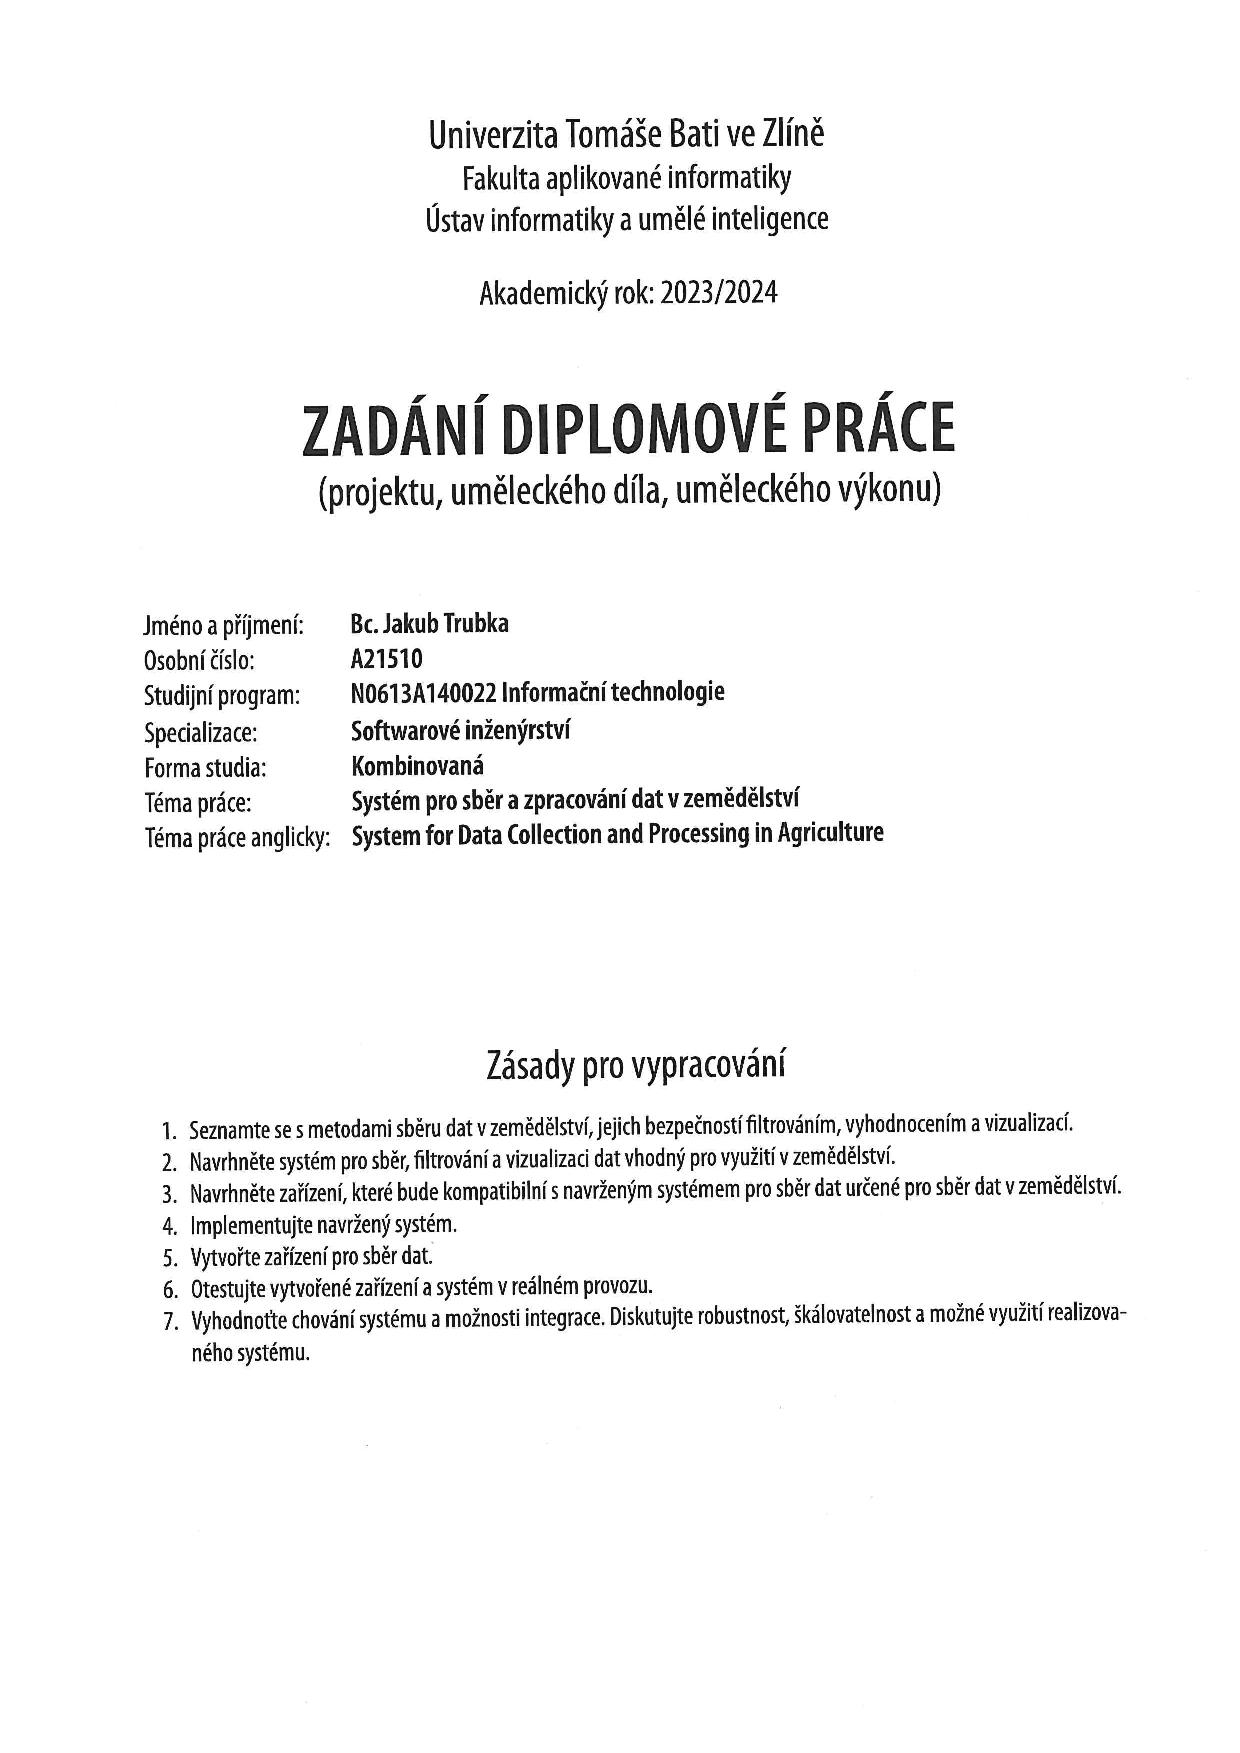
\includepdf[pages=-]{zadani.pdf}
	%*** Nascanované zadání, strana 1 ***
	
	%\clearpage
	%\thispagestyle{empty}
	%*** Nascanované zadání, strana 2 ***
}

% Nastaveni zobrazovani zahlavi dokumentu
\newcommand{\aktivujZahlavi}{
	\renewcommand{\headrulewidth}{1pt}
	\rhead{\thepage}
	
	\ifczech
		\lhead{\b{UTB ve Zlíně, \ifthenelse{\equal{\fakulta}{FAI}}{Fakulta aplikované informatiky}{\ifthenelse{\equal{\fakulta}{FAME}}{Fakulta managementu a ekonomiky}{\ifthenelse{\equal{\fakulta}{FHS}}{Fakulta humanitních studií}{\ifthenelse{\equal{\fakulta}{FLKR}}{Fakulta logistiky a krizového řízení}{\ifthenelse{\equal{\fakulta}{FMK}}{Fakulta multimediálních komunikací}{\ifthenelse{\equal{\fakulta}{FT}}{Fakulta technologická}{\ifthenelse{\equal{\fakulta}{UNI}}{Univerzitní institut}{}}}}}}}}}
	\else \ifenglish
		\lhead{\b{TBU in Zlín, \ifthenelse{\equal{\fakulta}{FAI}}{Faculty of Applied Informatics}{\ifthenelse{\equal{\fakulta}{FAME}}{Faculty of Management and Economics}{\ifthenelse{\equal{\fakulta}{FHS}}{Faculty of Humanities}{\ifthenelse{\equal{\fakulta}{FLKR}}{Faculty of Logistics and Crisis Management}{\ifthenelse{\equal{\fakulta}{FMK}}{Faculty of Multimedia Communications}{\ifthenelse{\equal{\fakulta}{FT}}{Faculty of Technology}{\ifthenelse{\equal{\fakulta}{UNI}}{University Institute}{}}}}}}}}}
	\fi \fi
}

% Příkaz \logopracerok vloží na dané místo logo fakulty, typ práce a rok
\newcommand{\logopracerok}{
	\ifczech
		\iffai	\put(82.2,-223.3){\makebox(84,16.4){
\includegraphics[width=90mm]{graphics/logo/fai_logo_cz.png}}} \fi
		\iffame	\put(82.2,-223.3){\makebox(84,16.4){
\includegraphics[width=90mm]{graphics/logo/fame_logo_cz.png}}} \fi
		\iffhs	\put(82.2,-223.3){\makebox(84,16.4){
\includegraphics[width=90mm]{graphics/logo/fhs_logo_cz.png}}} \fi
		\ifflkr	\put(82.2,-223.3){\makebox(84,16.4){
\includegraphics[width=90mm]{graphics/logo/flkr_logo_cz.png}}} \fi
		\iffmk	\put(82.2,-223.3){\makebox(84,16.4){
\includegraphics[width=90mm]{graphics/logo/fmk_logo_cz.png}}} \fi
		\ifft	\put(82.2,-223.3){\makebox(84,16.4){
\includegraphics[width=90mm]{graphics/logo/ft_logo_cz.png}}} \fi
		\ifuni	\put(82.2,-223.3){\makebox(84,16.4){
\includegraphics[width=90mm]{graphics/logo/uni_logo_cz.png}}} \fi
	\else \ifenglish
		\iffai	\put(82.2,-223.3){\makebox(84,16.4){
\includegraphics[width=90mm]{graphics/logo/fai_logo_en.png}}} \fi
		\iffame	\put(82.2,-223.3){\makebox(84,16.4){
\includegraphics[width=90mm]{graphics/logo/fame_logo_en.png}}} \fi
		\iffhs	\put(82.2,-223.3){\makebox(84,16.4){
\includegraphics[width=90mm]{graphics/logo/fhs_logo_en.png}}} \fi
		\ifflkr	\put(82.2,-223.3){\makebox(84,16.4){
\includegraphics[width=90mm]{graphics/logo/flkr_logo_en.png}}} \fi
		\iffmk	\put(82.2,-223.3){\makebox(84,16.4){
\includegraphics[width=90mm]{graphics/logo/fmk_logo_en.png}}} \fi
		\ifft	\put(82.2,-223.3){\makebox(84,16.4){
\includegraphics[width=90mm]{graphics/logo/ft_logo_en.png}}} \fi
		\ifuni	\put(82.2,-223.3){\makebox(84,16.4){
\includegraphics[width=90mm]{graphics/logo/uni_logo_en.png}}} \fi
	\fi \fi
	\put(0,-205){\linethickness{1pt}\line(1,0){170}}
	\ifczech
		\ifbp \put(4,-215){\makebox(69.5,4.5)[l]{\noindent\fontsize{16}{1}\usefont{OT1}{phv}{m}{n}Bakalářská práce}} \fi
		\ifdp \put(4,-215){\makebox(69.5,4.5)[l]{\noindent\fontsize{16}{1}\usefont{OT1}{phv}{m}{n}Diplomová práce}} \fi
	\else \ifenglish
		\ifbp \put(4,-215){\makebox(69.5,4.5)[l]{\noindent\fontsize{16}{1}\usefont{OT1}{phv}{m}{n}Bachelor's thesis}} \fi
		\ifdp \put(4,-215){\makebox(69.5,4.5)[l]{\noindent\fontsize{16}{1}\usefont{OT1}{phv}{m}{n}Master's thesis}} \fi
	\fi \fi
	\put(4,-220){\makebox(69.5,4.5)[l]{\noindent\fontsize{16}{1}\usefont{OT1}{phv}{m}{n}\rok}}
	\put(0,-225){\linethickness{1pt}\line(1,0){170}}
	\put(75,-223.3){\linethickness{1pt}\line(0,1){16.4}}
}

% Úvodní stránka s logem fakulty
\newcommand{\titulnistrana}{
	\thispagestyle{empty}
	\voffset=-2.01cm\evensidemargin=0pt\oddsidemargin=0cm\parindent=0pt\headsep=0pt\headheight=0pt\parskip=0pt\textheight=272mm\textwidth=200mm
	\renewcommand{\baselinestretch}{0}
	
	\setlength{\unitlength}{1mm}
	\begin{picture}(-10,8)
		\ifczech
			% Nazev prace
			%\put(0,-100){\makebox(170,50){\fontsize{24}{1}\usefont{OT1}{phv}{b}{n}#1}}
			%		\put(0,-100){\makebox(170,50){\protect\parbox{0.8\textwidth}{\protect\centering\fontsize{24}{1}\usefont{OT1}{phv}{b}{n}#1}}}
			
			% Vyreseno odradkovani
			\put(0,-100){\makebox(170,50){\protect\parbox{0.8\textwidth}{\protect\centering\setstretch{2.0}\usefont{OT1}{phv}{b}{n}{\Huge\nazevcz}}}}
			
			% Jmeno autora
			\put(0,-135){\makebox(170,25){\fontsize{20}{1}\usefont{OT1}{phv}{m}{n}\autor}}
		\else \ifenglish
			% Nazev prace
			%\put(0,-100){\makebox(170,50){\fontsize{24}{1}\usefont{OT1}{phv}{b}{n}#1}}
			%\put(0,-95){\makebox(170,50){\protect\parbox{0.8\textwidth}{\protect\centering\fontsize{24}{1}\usefont{OT1}{phv}{b}{n}#1}}}
			%\put(0,-88)%toto bylo pouzito v pripade zobrazeni nazvu ve dvou jazycich
			\put(0,-100){\makebox(170,50){\protect\parbox{0.8\textwidth}{\protect\centering\setstretch{2.0}\usefont{OT1}{phv}{b}{n}{\Huge\nazeven}}}}
	
			%\put(0,-111){\makebox(170,50){\fontsize{20}{1}\usefont{OT1}{phv}{m}{n}#1}}
			%\put(0,-116){\makebox(170,50){\protect\parbox{0.8\textwidth}{\protect\centering\fontsize{20}{1}\usefont{OT1}{phv}{m}{n}#2}}}
			%\put(0,-115){\makebox(170,50){\protect\parbox{0.8\textwidth}{\protect\centering\setstretch{1.5}\usefont{OT1}{phv}{m}{n}{\Large\nazevcz}}}}
			
			% Jmeno autora
			\put(0,-135){\makebox(170,25){\fontsize{20}{1}\usefont{OT1}{phv}{m}{n}\autor}}
		\fi \fi
		\logopracerok
	\end{picture}
}


% Strana s abstraktem a klíčovými slovy v češtině a angličtině
\newcommand{\abstraktaklicovaslova}{
	\clearpage
	\thispagestyle{empty}
	\nm{Abstrakt}
	\abstraktcz
	
	\vspace{1cm}
	Klíčová slova: \klicovaslovacz
	
	\vspace{3cm}
	
	\nns{Abstract}
	\abstrakten
	
	\vspace{1cm}
	Keywords: \klicovaslovaen
}


% ============================================================================ %
% NASTAVENÍ ZOBRAZENÍ PŘÍLOH -- SEZNAM, ČÍSLOVÁNÍ, VLASTNÍ STYL

\makeatletter % tímto příkazem dávám najevo, že budu editovat přímo příkazy ze šablony

% definice seznamu příloh - příkaz \listofappendices
\def\listofappendices{%
	\newpage
	\phantomsection
	\setcounter{section}{0}
	\ifczech
		\addcontentsline{toc}{section}{Seznam příloh}
		\@restonecolfalse\if@twocolumn\@restonecoltrue\onecolumn\fi
		\section*{SEZNAM PŘÍLOH}
	\else \ifenglish
		\addcontentsline{toc}{section}{List of Appendices}
		\@restonecolfalse\if@twocolumn\@restonecoltrue\onecolumn\fi
		\section*{LIST OF APPENDICES}
	\fi \fi
	\@mkboth{LIST OF APPENDICES}{LIST OF APPENDICES}
	\@starttoc{loa}\if@restonecol\twocolumn\fi
	\pagestyle{empty}
	\thispagestyle{fancy}
}

\def\ext@appendix{loa}
\def\tocname{loa}

% definice příkazu \priloha{nazev prilohy} pro vložení nové přílohy
\newcommand{\priloha}[1]{
	\clearpage
	\refstepcounter{section}
	%\voffset=-3cm % vertikalni posun
	\addtocontents{loa}{\protect\makebox[1.5cm][l]{\ifczech P\else \ifenglish A\fi\fi\ \@Roman\c@section.} #1\newline}
	\ifczech
		{\bf PŘÍLOHA \ifczech P\else \ifenglish A\fi\fi\ \@Roman\c@section. \MakeTextUppercase{#1}}
	\else \ifenglish
		{\bf APPENDIX \ifczech P\else \ifenglish A\fi\fi\ \@Roman\c@section. \MakeTextUppercase{#1}}
	\fi \fi
	\par
}

% ============================================================================ %
% OBSAH: NASTAVENÍ VELKÝCH PÍSMEN PRO NÁZVY SEKCÍ A HLAVNÍCH NADPISŮ

\let\oldcontentsline\contentsline
\def\contentsline#1#2{%
	\expandafter\ifx\csname l@#1\endcsname\l@section
		\expandafter\@firstoftwo
	\else
		\expandafter\@secondoftwo
	\fi
	{%
		\oldcontentsline{#1}{\MakeTextUppercase{#2}}%
	}{%
		\oldcontentsline{#1}{#2}%
	}%
}

\def\@part[#1]#2{
	\ifnum \c@secnumdepth >\m@ne
		\refstepcounter{part}
		\addcontentsline{toc}{section}{\protect\texorpdfstring{\makebox[0.85cm]{\thepart\hfill} #1}{\thepart\ #1}}
	\else
		\addcontentsline{toc}{section}{#1}
	\fi
	{\parindent \z@ \raggedright
	\interlinepenalty \@M
	\clearpage
	\normalfont
	\ifnum \c@secnumdepth >\m@ne
		\Large\bfseries
		\nobreak
	\fi
	\vspace*{9cm}
	\center\huge \bfseries\thepart. \MakeTextUppercase{#2}
	\markboth{}{}\par}
	\nobreak
	\clearpage
	\@afterheading
}


% ============================================================================ %
% NASTAVENÍ FORMÁTU ČÍSLOVÁNÍ OBRÁZKŮ A TABULEK

\def\thefigure{\arabic{figure}}	% číslování obrázků typu (y)
\def\thetable{\arabic{table}}	% číslování tabulek typu (y)
\captiondelim{. } % změníme dvoutečku za Obr/Tab za tečku

% Nastavení číslování obrázků, tabulek i rovnic do formátu <číslo kapitoly>.<pořadové číslo>
\counterwithin{figure}{section}
\counterwithin{table}{section}
\counterwithin{equation}{section}

% Odsazeni popisku v seznamu obrazku a tabulek
\patchcmd{\@caption}{\csname the#1\endcsname}{\csname fnum@#1\endcsname}{}{}
%{\renewcommand*\numberline[1]{Fig. \,#1\space}}
%\renewcommand*\l@figure{\@dottedtocline{1}{0em}{5.0em}}
%\renewcommand*\l@table{\@dottedtocline{1}{0em}{5.0em}}

% Vynulování čítačů
\@addtoreset{table}{section}
\@addtoreset{figure}{section}
\@addtoreset{footnote}{section}

\makeatother % a to je ukončení \makeatletter


% ============================================================================ %
% ÚPRAVA VZHLEDU OBSAHU, SEZNAMU OBRÁZKŮ A TABULEK

% nastavení vertikální mezery před stylem část, nadpis 1--3
\setlength{\cftbeforepartskip}{3pt}
\setlength{\cftbeforesecskip}{3pt}
\setlength{\cftbeforesubsecskip}{3pt}
\setlength{\cftbeforesubsubsecskip}{0cm}

% odsazení zleva pro styl část, nadpis 1--3
\setlength{\cftpartindent}{0cm}
\setlength{\cftsecindent}{0cm}
\setlength{\cftsubsecindent}{0cm}
\setlength{\cftsubsubsecindent}{0cm}

% nastavení fontu pro styl část, nadpis 1--3
\renewcommand{\cftpartfont}{\small\bfseries}
\renewcommand{\cftsecfont}{\small\bfseries}
\renewcommand{\cftsubsecfont}{\scshape}
\renewcommand{\cftsubsubsecfont}{}

% odsazení čísla a textu titulku pro styl část, nadpis 1--3
\cftsetindents{part}{0cm}{1cm}
\cftsetindents{sec}{0cm}{1cm}
\cftsetindents{subsec}{0.5cm}{1.25cm}
\cftsetindents{subsubsec}{1cm}{1.5cm}
\cftsetindents{fig}{0cm}{1.5cm}
\cftsetindents{tab}{0cm}{1.5cm}

% nastavení vodící čáry pro styl část, nadpis 1--3, obrázky a tabulky
\renewcommand{\cftdot}{\ensuremath{.}} % tímto příkazem lze změnit vodící tečky v obsahu na jiný znak
\renewcommand{\cftpartleader}{\cftdotfill{0.3}}
\renewcommand{\cftsecleader}{\cftdotfill{0.3}}
\renewcommand{\cftsubsecleader}{\cftdotfill{0.3}}
\renewcommand{\cftsubsubsecleader}{\cftdotfill{0.3}}
\renewcommand{\cftfigleader}{\cftdotfill{0.3}}
\renewcommand{\cfttableader}{\cftdotfill{0.3}}

% změna fontu pro text "Obsah", "Seznam obrázků" a "Seznam tabulek"
\renewcommand{\cfttoctitlefont}{\normalsize\bfseries\thispagestyle{empty}}
\renewcommand{\cftloftitlefont}{\normalsize\bfseries\thispagestyle{fancy}}
\renewcommand{\cftlottitlefont}{\normalsize\bfseries\thispagestyle{fancy}}

\renewcommand{\cfttabpresnum}{Tab. }
\renewcommand{\cftfigaftersnum}{.}
\renewcommand{\cfttabaftersnum}{.}
\setlength{\cftfignumwidth}{5em}
\setlength{\cfttabnumwidth}{5em}


% ============================================================================ %
% NASTAVENÍ FONTU PRO NADPISY

\sectionfont{\normalsize}
\subsectionfont{\normalsize\bfseries}
\subsubsectionfont{\small\bfseries}
\paragraphfont{\small\bf}

% definice nového stylu \comment -- komentář k šabloně
\newcommand{\comment}[1]{\color{red}#1\color{black}}


% ============================================================================ %
% VSTUPY

% Nastaveni a kontrola fakulty
\newcommand{\nastavfakultu}[1]{
	\newcommand{\fakulta}{#1}
	\newif\iffai	\let\iffai\iffalse
	\newif\iffame	\let\iffame\iffalse
	\newif\iffhs	\let\iffhs\iffalse
	\newif\ifflkr	\let\ifflkr\iffalse
	\newif\iffmk	\let\iffmk\iffalse
	\newif\ifft		\let\ifft\iffalse
	\newif\ifuni	\let\ifuni\iffalse
	
	\ifthenelse{\equal{#1}{FAI}}{\let\iffai\iftrue}{}
	\ifthenelse{\equal{#1}{FAME}}{\let\iffame\iftrue}{}
	\ifthenelse{\equal{#1}{FHS}}{\let\iffhs\iftrue}{}
	\ifthenelse{\equal{#1}{FLKR}}{\let\ifflkr\iftrue}{}
	\ifthenelse{\equal{#1}{FMK}}{\let\iffmk\iftrue}{}
	\ifthenelse{\equal{#1}{FT}}{\let\ifft\iftrue}{}
	\ifthenelse{\equal{#1}{UNI}}{\let\ifuni\iftrue}{}
	
	\iffai \else \iffame \else \iffhs \else \ifflkr \else \iffmk \else \ifft \else \ifuni \else
		\errmessage{Chyba nastaveni fakulty}
	\fi \fi \fi \fi \fi \fi \fi
}

% Nastaveni a kontrola typu prace
\newcommand{\nastavtyp}[1]{
	\newcommand{\typ}{#1}
	
	\newif\ifbp \let\ifbp\iffalse
	\newif\ifdp \let\ifdp\iffalse
	
	\ifthenelse{\equal{#1}{BP}}{\let\ifbp\iftrue}{}
	\ifthenelse{\equal{#1}{DP}}{\let\ifdp\iftrue}{}
	
	\ifbp \else \ifdp \else
		\errmessage{Chyba nastaveni typu prace}
	\fi \fi
}

% Nastaveni roku
\newcommand{\nastavrok}[1]{
	\newcommand{\rok}{#1}
}

% Nastaveni jmena
\newcommand{\nastavautora}[1]{
	\newcommand{\autor}{#1}
}

% Nastaveni nazvu
\newcommand{\nastavnazevcz}[1]{
	\newcommand{\nazevcz}{#1}
}
\newcommand{\nastavnazeven}[1]{
	\newcommand{\nazeven}{#1}
}

% Nastaveni abstraktu
\newcommand{\nastavabstraktcz}[1]{
	\newcommand{\abstraktcz}{#1}
}
\newcommand{\nastavabstrakten}[1]{
	\newcommand{\abstrakten}{#1}
}

% Nastaveni klicovych slov
\newcommand{\nastavklicovaslovacz}[1]{
	\newcommand{\klicovaslovacz}{#1}
}
\newcommand{\nastavklicovaslovaen}[1]{
	\newcommand{\klicovaslovaen}{#1}
}

% Nastaveni a kontrola jazyka
\newcommand{\nastavjazyk}[1]{
	\newcommand{\jazyk}{#1}
	
	\newif\ifczech		\let\ifczech\iffalse
	\newif\ifenglish	\let\ifenglish\iffalse
	
	\ifthenelse{\equal{#1}{CZ}}{\let\ifczech\iftrue}{}
	\ifthenelse{\equal{#1}{EN}}{\let\ifenglish\iftrue}{}
	
	\ifczech \else \ifenglish \else
		\errmessage{Chyba nastaveni jazyka}
	\fi \fi
	
	\ifczech
		\usepackage[czech]{babel}
		% Vlastni definice nazvu
		\addto\captionsczech{\renewcommand{\contentsname}{\MakeTextUppercase{Obsah}}}
		\addto\captionsczech{\renewcommand{\refname}{\MakeTextUppercase{Seznam použité literatury}}}
		\addto\captionsczech{\renewcommand{\listfigurename}{\MakeTextUppercase{Seznam obrázků}}}
		\addto\captionsczech{\renewcommand{\listtablename}{\MakeTextUppercase{Seznam tabulek}}}
		%\addto\captionsczech{\renewcommand{\figurename}{Obr.}}
		%\addto\captionsczech{\renewcommand{\tablename}{Tab.}}
		\renewcommand{\cftfigpresnum}{Obr. }
	\else \ifenglish
		\usepackage[english]{babel}	
		% Vlastni definice nazvu
		\addto\captionsenglish{\renewcommand{\contentsname}{\MakeTextUppercase{Table of Contents}}}
		\addto\captionsenglish{\renewcommand{\refname}{\MakeTextUppercase{References}}}
		\addto\captionsenglish{\renewcommand{\listfigurename}{\MakeTextUppercase{List of Figures}}}
		\addto\captionsenglish{\renewcommand{\listtablename}{\MakeTextUppercase{List of Tables}}}
		%\addto\captionsenglish{\renewcommand{\figurename}{Fig.}}
		%\addto\captionsenglish{\renewcommand{\tablename}{Tab.}}
		\renewcommand{\cftfigpresnum}{Fig. }
	\fi \fi
}


% Nastaveni vertikalniho odsazeni nad rovnicemi/soustavami rovnic (prvni parametr),
% a pod (druhy parametr)
\newcommand{\nastavmezerukolemrovnic}[2]{
	\let\oldequation=\equation
	\let\endoldequation=\endequation
	\renewenvironment{equation}{\vspace{#1}\begin{oldequation}}{\end{oldequation}\vspace{#2}}
	
	\let\oldeqnarray=\eqnarray
	\let\endoldeqnarray=\endeqnarray
	\renewenvironment{eqnarray}{\vspace{#1}\begin{oldeqnarray}}{\end{oldeqnarray}\vspace{#2}}
}

% Nastaveni vertikalniho odsazeni nad tabulkami (prvni parametr),
% a pod (druhy parametr)
\newcommand{\nastavmezerukolemtabulek}[2]{
	\let\oldtable=\table
	\let\endoldtable=\endtable
	\renewenvironment{table}{\vspace{#1}\begin{oldtable}}{\end{oldtable}\vspace{#2}}
}

% Nastaveni vertikalniho odsazeni nad obrazky (prvni parametr),
% a pod (druhy parametr)
\newcommand{\nastavmezerukolemobrazku}[2]{
	\let\oldfigure=\figure
	\let\endoldfigure=\endfigure
	\renewenvironment{figure}{\vspace{#1}\begin{oldfigure}}{\end{oldfigure}\vspace{#2}}
}


% ============================================================================ %
% STRANA S PROHLASENIM

\newcommand{\prohlaseni}{{
	\clearpage
	\thispagestyle{empty}

	\ifczech
	\textbf{Prohlašuji, že}
	\begin{itemize}
		\setlength{\parskip}{0pt}
		\setlength{\itemsep}{0pt}
		\setstretch{1.05}
		\item{beru na vědomí, že odevzdáním \ifbp bakalářské \else \ifdp diplomové \fi \fi práce souhlasím se zveřejněním své práce podle zákona č. 111/1998 Sb. o vysokých školách a o změně a doplnění dalších zákonů (zákon o vysokých školách), ve znění pozdějších právních předpisů, bez ohledu na výsledek obhajoby;}
		\item{beru na vědomí, že \ifbp bakalářské \else \ifdp diplomové \fi \fi práce bude uložena v elektronické podobě v univerzitním informačním systému dostupná k prezenčnímu nahlédnutí, že jeden výtisk \ifbp bakalářské \else \ifdp diplomové \fi \fi práce bude uložen v příruční knihovně \iffai Fakulty aplikované informatiky. \else \iffame Fakulty managementu a ekonomiky. \else \iffhs Fakulty humanitních studií. \else \ifflkr Fakulty logistiky a krizového řízení. \else \iffmk Fakutly mutimediálních komunikací. \else \ifft Fakulty technologické. \else \ifuni Univerzitního institutu. \if \fi \fi \fi \fi \fi \fi \fi \fi Univerzity Tomáše Bati ve Zlíně; }
		\item{byl/a jsem seznámen/a s tím, že na moji \ifbp bakalářskou \else \ifdp diplomovou \fi \fi práci se plně vztahuje zákon č. 121/2000 Sb. o právu autorském, o právech souvisejících s právem autorským a o změně některých zákonů (autorský zákon) ve znění pozdějších právních předpisů, zejm. § 35 odst. 3;}
		\item{beru na vědomí, že podle § 60 odst. 1 autorského zákona má Univerzita Tomáše Bati ve Zlíně právo na uzavření licenční smlouvy o užití školního díla v rozsahu § 12 odst. 4 autorského zákona;}
		\item{beru na vědomí, že podle § 60 odst. 2 a 3 autorského zákona mohu užít své dílo –\ \ifbp bakalářskou \else \ifdp diplomovou \fi \fi práci nebo poskytnout licenci k~jejímu využití jen připouští-li tak licenční smlouva uzavřená mezi mnou a Univerzitou Tomáše Bati ve Zlíně s~tím, že vyrovnání případného přiměřeného příspěvku na úhradu nákladů, které byly Univerzitou Tomáše Bati ve Zlíně na vytvoření díla vynaloženy (až do jejich skutečné výše) bude rovněž předmětem této licenční smlouvy;}
		\item{beru na vědomí, že pokud bylo k vypracování \ifbp bakalářské \else \ifdp diplomové \fi \fi práce využito softwaru poskytnutého Univerzitou Tomáše Bati ve Zlíně nebo jinými subjekty pouze ke~studijním a výzkumným účelům (tedy pouze k~nekomerčnímu využití), nelze výsledky \ifbp bakalářské \else \ifdp diplomové \fi \fi práce využít ke komerčním účelům;}
		\item{beru na vědomí, že pokud je výstupem \ifbp bakalářské \else \ifdp diplomové \fi \fi práce jakýkoliv softwarový produkt, považují se za součást práce rovněž i zdrojové kódy, popř. soubory, ze kterých se projekt skládá. Neodevzdání této součásti může být důvodem k~neobhájení práce.}
	\end{itemize}
	\medskip
	%\clearpage
	%\thispagestyle{empty}
	\textbf{Prohlašuji,}
	\begin{itemize}
		\setlength{\parskip}{0pt}
		\setlength{\itemsep}{0pt}
		\setstretch{1.05}
		\item{že jsem na \ifbp bakalářské \else \ifdp diplomové \fi \fi práci pracoval samostatně a použitou literaturu jsem citoval. V případě publikace výsledků budu uveden jako spoluautor.}
		\item{že odevzdaná verze \ifbp bakalářské \else \ifdp diplomové \fi \fi práce a verze elektronická nahraná do IS/STAG jsou totožné.}
	\end{itemize}
	\medskip
	Ve Zlíně, dne \hspace{6.5cm}\dots\dots\dots\dots\dots\dots\dots\dots\dots\dots
	
	\hspace{10.3cm}podpis studenta
	
	\else \ifenglish
	%\nm{THESIS AUTHOR STATEMENT}
	\textbf{I hereby declare that:}
	\begin{itemize}
		\setlength{\parskip}{0pt}
		\setlength{\itemsep}{0pt}
		\setstretch{1.05}
		\item{I understand that by submitting my \ifbp Bachelor's \else\ifdp Master's \fi\fi thesis, I agree to the publication of my work according to Law No. 111/1998, Coll., On Universities and on changes and amendments to other acts (e.g. the Universities Act), as amended by subsequent legislation, without regard to the results of the defence of the thesis.}		
		\item{I understand that my \ifbp Bachelor's \else\ifdp Master's \fi\fi Thesis will be stored electronically in the university information system and be made available for on-site inspection, and that a copy of the \ifbp Bachelor's \else\ifdp Master's \fi\fi Thesis will be stored in the Reference Library of the 
		\iffai Faculty of Applied Informatics, \else\iffame Faculty of Management and Economics, \else \iffhs Faculty of Humanities, \else\ifflkr Faculty of Logistics and Crisis Management, \else\iffmk Faculty of Multimedia Communications, \else\ifft Faculty of Technology, \else\ifuni University Institute, \if \fi \fi \fi \fi \fi \fi \fi \fi Tomas Bata University in Zlín.}
		\item{I am aware of the fact that my \ifbp Bachelor's \else\ifdp Master's \fi\fi Thesis is fully covered by Act No. 121/2000 Coll. On Copyright, and Rights Related to Copyright, as amended by some other laws (e.g. the Copyright Act), as amended by subsequent legislation; and especially, by §35, Para. 3.}
		\item{I understand that, according to §60, Para. 1 of the Copyright Act, Tomas Bata University in Zlín has the right to conclude licensing agreements relating to the use of scholastic work within the full extent of §12, Para. 4, of the Copyright Act.}
		\item{I understand that, according to §60, Para. 2, and Para. 3, of the Copyright Act, I may use my work – \ifbp Bachelor's \else\ifdp Master's \fi\fi Thesis, or grant a license for its use, only if permitted by the licensing agreement concluded between myself and Tomas Bata University in Zlín with a view to the fact that Tomas Bata University in Zlín must be compensated for any reasonable contribution to covering such expenses/costs as invested by them in the creation of the thesis (up until the full actual amount) shall also be a subject of this licensing agreement.}
		\item{I understand that, should the elaboration of the \ifbp Bachelor's \else\ifdp Master's \fi\fi Thesis include the use of software provided by Tomas Bata University in Zlín or other such entities strictly for study and research purposes (i.e. only for non-commercial use), the results of my \ifbp Bachelor's \else\ifdp Master's \fi\fi Thesis cannot be used for commercial purposes.}
		\item{I understand that, if the output of my \ifbp Bachelor's \else\ifdp Master's \fi\fi Thesis is any software product(s), this/these shall equally be considered as part of the thesis, as well as any source codes, or files from which the project is composed. Not submitting any part of this/these component(s) may be a reason for the non-defence of my thesis.}
	\end{itemize}
	\medskip
	%\clearpage
	%\thispagestyle{empty}
	\textbf{I herewith declare that:}
	\begin{itemize}
		\setlength{\parskip}{0pt}
		\setlength{\itemsep}{0pt}
		\setstretch{1.05}
		\item{I have worked on my thesis alone and duly cited any literature I have used. In the case of the publication of the results of my thesis, I shall be listed as co-author.}
		\item{The submitted version of the thesis and its electronic version uploaded to IS/STAG are both identical.}
	\end{itemize}
	\medskip
	In Zlín; dated: \hspace{6.5cm}\dots\dots\dots\dots\dots\dots\dots\dots\dots\dots

	\hspace{10.3cm}Student's Signature
	
	\fi \fi
}}

% ============================================================================ %


% Uživatelské definice -- upravte dle požadavků
\nastavfakultu{FAI}
	% FAI  -- pro Fakultu aplikované informatiky
	% FAME -- pro Fakultu managementu a ekonomiky
	% FHS  -- pro Fakultu humanitních studií
	% FLKR -- pro Fakultu logistiky a krizového řízení
	% FMK  -- pro Fakutlu mutimediálních komunikací
	% FT   -- pro Fakultu technologickou
	% UNI  -- pro Univerzitní institut
\nastavtyp{DP}
	% BP   -- bakalářská práce
	% DP   -- diplomová práce
\nastavrok{2024}
	% zadejte rok místo "xxxx"
\nastavjazyk{CZ}
	% CZ   -- práce bude v českém jazyce
	% EN   -- práce bude v anglickém jazyce

% Lze přidat vertikalni odsazeni nad (prvni parametr) a pod (druhy parametr)
% obrázky, tabulky i rovnice/soustavy rovnic
\nastavmezerukolemobrazku{0mm}{0mm}
\nastavmezerukolemtabulek{0mm}{0mm}
\nastavmezerukolemrovnic{0mm}{0mm}

\nastavautora{Bc. Jakub Trubka}
\nastavnazevcz{Systém pro sběr a zpracování dat v zemědělství}
\nastavnazeven{Název práce anglicky (max. 2 řádky)} % Jen u anglicky psané práce
\nastavabstraktcz{Tato diplomová práce se zabývá návrhem a implementací systému pro sběr, zpracování, uchovávání a vizualizaci dat získaných v oblasti zemědělství, primárně v oblasti sadařství a vinařství.  Výsledný systém umožňuje uživateli monitorování podmínek v místě umístění zařízení se senzory. Systém klade důraz na nízkou cenu, odolnost a rozšiřitelnost. V rámci teoretické části jsou popsána existující řešení a rozebrána problematika sběru, zpracování a vizualizace dat. Praktická část se věnuje návrhu architektury systému, včetně návrhu jednotlivých zařízení pro sběr dat a komunikačních protokolů. Dále se praktická část zabývá implementací celého systému a jeho jednotlivých částí. V práci jsou též diskutovány výsledky získané experimentováním s vytvořeným systémem a diskutovány další možnosti zlepšení systému jako takového.
}
\nastavabstrakten{This thesis deals with the design and implementation of a system for collection, processing, storage and visualization of data obtained in the field of agriculture, primarily in the field of orchards and viticulture. The resulting system allows the user to monitor the conditions at the location of the device with sensors. The system emphasizes low cost, durability, and expandability. In the theoretical part, existing solutions are described and the issues of data collection, processing and visualization are analyzed. The practical part is devoted to the design of the system architecture, including the design of individual devices for data collection and communication protocols. Furthermore, the practical part deals with the implementation of the entire system and its individual parts. The work also discusses the results obtained by experimenting with the created system and discusses other possibilities for improving the system as such.}
\nastavklicovaslovacz{IoT, sběr dat, analýza dat, vizualizace dat, LoRa, MQTT, InfluxDB, zemědělství, senzory}
\nastavklicovaslovaen{IoT, data collection, data analysis, data visualization, LoRa, MQTT, InfluxDB, agriculture, sensors}

% Následující příkaz nastaví standard PDF/A-1b
\aplikujpdfa


% ============================================================================ %
\begin{document}

\titulnistrana

\zadani
%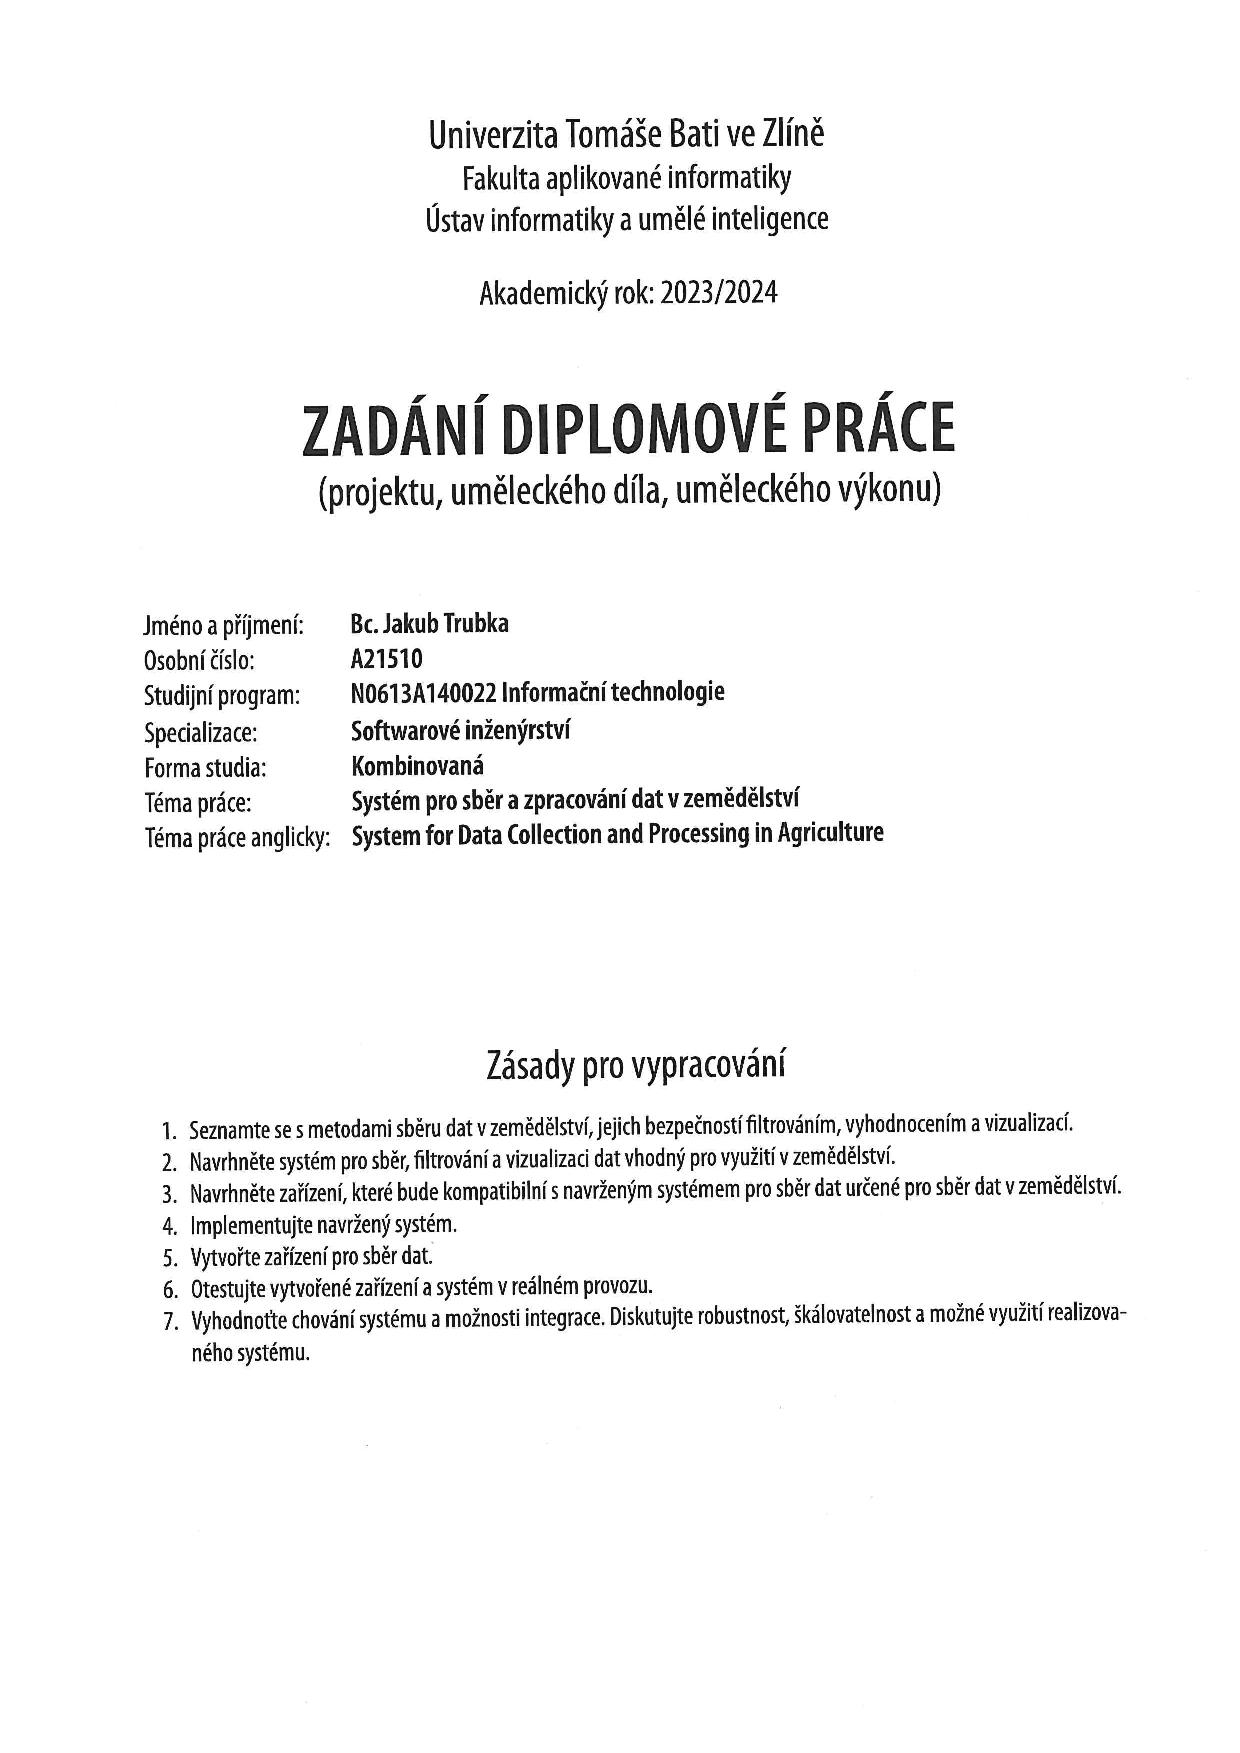
\includepdf[pages=-]{zadani.pdf}

\prohlaseni

\abstraktaklicovaslova


% ============================================================================ %
\clearpage
\thispagestyle{empty}
Děkuji vedoucímu diplomové práce Ing. Pavlovi Vařachovi, Ph.D. za rady, trpělivost a ochotu při konzultacích. Poděkování patří také Vinařskému spolku Uherčice za poskytnutí prostor k testování systému.



% ============================================================================ %
\obsah  % Obsah je generován automaticky


% ============================================================================ %
\OdsazovaniOdstavcuStart % Nastaví odsazování odstavců dle zvoleného jazyka

% ============================================================================ %
% Encoding: UTF-8 (žluťoučký kůň úpěl ďábelšké ódy)
% ============================================================================ %

% ============================================================================ %
\nn{Úvod}
Zemědělství reprezentuje jedno z~klíčových odvětví světové ekonomiky, zajišťuje potraviny, krmivo a paliva pro miliardy lidí. Nicméně čelí řadě komplexních výzev, včetně růstu populace, změny klimatu, nedostatku zdrojů, degradace životního prostředí a nestálosti na trhu. Prostředkem k~řešením těchto výzev může být i~zavádění moderních technologií a~inovativních přístupů, které by mohli vylepšit produktivitu, efektivitu a udržitelnost zemědělství.

Jedním z~moderních přístupů je sběr a analýza dat v~zemědělství. Tento proces zahrnuje shromažďování, zpracování a interpretaci různých dat spojených se zemědělskými aktivitami. Mezi tato data patří například údaje o~růstu plodin, stavu půdy, povětrnostních podmínkách, škůdcích a řízení farmy. Sběr a analýza dat mohou výrazně podpořit rozhodovací procesy zemědělců a dalších zainteresovaných stran, optimalizovat vstupy, snižovat náklady, zvyšovat kvalitu a výnosy. Taktéž mohou přispět k~tvorbě politik, vědeckému výzkumu a vzdělávání v~oblasti zemědělství. Ač se tyto technologie stávají stále dostupnější, jsou velmi nákladné. To není problém pro velké zemědělské provozy, které zavedením moderních procesů mohou zvýšením efektivity ušetřit nemalé sumy, problém ovšem nastává u~menších zemědělců. Zvýšení efektivity u~nich nevyrovná náklady na pořízení moderních systémů pro sběr a analýzu dat. Existující systémy jsou však zaměřené především na větší provozy.

Hlavním cílem této práce je vyvinout systém pro sběr a analýzu dat v~zemědělství, který nabídne spolehlivé, bezpečné a uživatelsky přívětivé řešení pro sběr, filtrování a vizualizaci zemědělských dat. Práce si bere zároveň za cíl, aby celý systém byl transparentní, modulární, veřejně dostupný a levný na údržbu i nasazení. Systém se skládá ze dvou hlavních částí, zařízení pro sběr dat a platformy pro analýzu dat. Zařízení pro sběr dat je fyzické zařízení osazené senzory, určené k~měření. Platforma pro analýzu dat je softwarová platforma, která přijímá, ukládá, filtruje a vizualizuje data shromážděná zařízením.

Práce obsahuje teoretickou část, ve které je popsána aktuální situace \ref{sec:actual_situation} a používané technologie \ref{sec:used_technologies}. Sekce o~aktuální situaci si bere za cíl seznámit čtenáře s~problematikou sběru dat v~zemědělství, používanými senzory a existujícími řešeními. Sekce věnující se používaným technologiím seznamuje čtenáře s~problematikou IoT a analýzou dat. 

Dále práce obsahuje praktickou část, která obsahuje sekce věnující se návrhu \ref{sec:system_design}, implementaci \ref{sec:impelementation} a testování systému \ref{sec:testing}. Návrh systému obsahuje mimo jiné i případy užití a specifikace požadavků, ze kterých vychází celý návrh, implementace i testování.


% ============================================================================ %
\cast{Teoretická část}

\n{1}{Aktuální situace} \label{sec:actual_situation}
V~dnešní době zaujímá získávání a správa dat klíčovou roli ve vývoji a optimalizaci různých odvětví lidské činnosti. Nasbíraná data umožňují analyzovat a optimalizovat různé výrobní procesy, zlepšovat kvalitu produktů a služeb, předvídat a řešit problémy a zvyšovat konkurenceschopnost. Například monitorování průmyslového stroje pomocí senzorů může včas odhalit jeho poruchu a zabránit tak zbytečným výpadkům ve výrobě, které by mohly způsobit ztrátu času, peněz či ohrožení lidských životů.

Zemědělství je jedním z~odvětví, kde se sběr a zpracování dat stává stále důležitějším a rozšířenějším. Data mohou poskytnout zemědělcům cenné informace, které jim pomáhají při rozhodování o~různých aspektech zemědělské produkce, jako je výběr vhodných rostlin, stanovení optimálních termínů výsevu a sklizně, aplikace hnojiv a pesticidů, zavlažování a další. Data také umožňují sledovat a hodnotit podmínky růstu plodin, jejich výnosnost, odolnost vůči škůdcům a chorobám. Správné využití získaných dat může výrazně zvýšit efektivitu a udržitelnost zemědělského hospodaření a zpracování plodin. Podrobnější informace o~sběru dat v~zemědělství jsou uvedeny v~podkapitole \ref{1_1_data_collection}. 

Zdroje dat v~zemědělství mohou být různého druhu. Mezi nejčastější patří různé typy senzorů, které měří například teplotu, vlhkost, kyselost a složení půdy, koncentraci živin, intenzitu světla a další parametry. Dalším zdrojem dat jsou satelitní a letecké snímky, které poskytují informace o~rozloze, typu a stavu plodin, erozi půdy, znečištění vody a ovzduší a dalších faktorech. Kromě toho existují i administrativní záznamy, jako jsou statistiky, smlouvy, certifikáty, dotace a další dokumenty, které se týkají zemědělské činnosti. Získání dat z~těchto zdrojů je v~současnosti snadné a dostupné. Ceny senzorů a dalších zařízení pro sběr dat neustále klesají, zatímco jejich kvalita a spolehlivost rostou. Na trhu se objevuje stále více společností, které se specializují na sběr a zpracování dat v~zemědělství a nabízejí zemědělcům různé služby a aplikace. Existují i veřejně dostupné služby, které umožňují získávat satelitní snímky půdy zdarma nebo za nízký poplatek. Příklady takovýchto společností a služeb jsou popsány v~podkapitole \ref{1_2_existing_solutions}.

\n{2}{Sběr dat v~zemědělství}\label{1_1_data_collection}
Sběr dat v~zemědělství je složitý proces, který zahrnuje mnoho různých typů dat. Zemědělec obvykle nemá k~dispozici jediné řešení, které by pokrývalo všechny jeho potřeby. Zemědělská technika obsahuje spoustu senzorů, ovšem data z~nich se nesbírají. Při sklizni se sbírá informace o~výnosu z~daného místa, ale tyto informace nejsou spojeny s~množstvím srážek či se složením půdy. To, že neexistují kompletní systémy pro sběr a zpracování dat, omezuje potenciál využití moderních digitálních technologií \cite{BDIA_POV1}. V~oblasti zemědělství se setkáváme s~několika problémy, které brání plnému využití potenciálu dat a informací, které lze z~nich získat. Tyto problémy se týkají zejména fragmentace, standardizace, sdílení a dostupnosti dat \cite{DCAP}\cite{BDPP}.

\n{3}{Problémy}
Informace z~této podsekce jsou čerpány z~\cite{DCAP}. Prvním problémem je fragmentace dat. Zemědělská data zahrnují údaje o~půdě, plodinách, podmínkách, škůdcích logistice a podobně. Moderní technologie a přístupy postupně umožňují sledování všech těchto informací, problémem ovšem i nadále zůstává izolovanost a kompatibilita těchto datových sad a systémů, které datové sady spravují. Například údaje o~výnosu plodiny získané při sklizni sbírá pro zemědělce výrobce strojů provádějících sklizeň, zatímco sběr informací o~úhrnu srážek obstarává jiný systém a jejich propojení není triviální. Tato fragmentace dat stěžuje jejich analýzu, která by mohla poskytnout ucelený pohled.

Druhým problémem je nedostatečná standardizace. Data jsou ukládána různými systémy, různými způsoby a v~různých formátech. Tento problém zásadně znesnadňuje integrace datových sad do rozsáhlejších systémů a spolupráci různých systémů. Nedostatek standardů také zvyšuje nároky na kvalitu a spolehlivost dat, která musí být ověřována a validována před jejich použitím. Standardizace dat by usnadnila jejich výměnu, porovnávání a kombinování.

Tímto se dostáváme ke třetímu problému a tím je omezení sdílení dat. Nasbíraná data jsou často pouze lokálního rázu a neumožňují pohled v~širším měřítku.  Pokud by byla data sdílena mezi různými zemědělci, výzkumníky, poradci, úřady a dalšími zainteresovanými stranami, bylo by možné vytvářet přesnější modely a predikce, které by pomohly zlepšit zemědělskou praxi a politiku. Sdílení dat by také podporovalo spolupráci a inovaci v~zemědělství.

Posledním problémem je také dostupnost vyhodnocovacích systémů. I~přes to, že různé senzory a data jsou dostupnější než kdy dřív, je potřeba tato data vyhodnocovat. Toto může být problém pro menší zemědělce, kterým se nevyplatí kvůli drobnému zvýšení efektivity platit vyšší částky za analýzu dat. Tito drobní zemědělci nejsou pro společnosti zabývající se zpracováním těchto dat lukrativní.

\n{3}{Metody sběru dat}
Ke sběru dat v~zemědělství se primárně používaly tradiční techniky, jako jsou terénní průzkumy, odběry vzorků půdy, laboratorní analýzy a experimenty. Tyto metody jsou užitečné pro získání průměrů a rozptylů parametrů plodin a půdy, ale mají některá omezení, jako jsou vysoké náklady, pracnost, spotřeba času a nízké prostorové rozlišení. Již delší dobu se využívají přesné metody sběru dat založeny na nových technologiích, jako je dálkový průzkum země, globální polohový systém (GPS), geografické informační systémy (GIS) a senzory. Tyto metody jsou schopny lépe zachytit časovou a prostorovou změnu podmínek a stavů a zlepšit produktivitu v~zemědělství. \cite{shibusawa2009data} 

Při dálkovém průzkumu země se získávají informace bez fyzického kontaktu s~objektem. Dálkový průzkum lze provádět pomocí různých platforem, jako jsou například družice či letadla. Dálkový průzkum poskytuje informace o~různých parametrech plodin a půdy v~zemědělství. Data pořízená při leteckém či satelitním snímkování se vyhodnocují specializovanými algoritmy pro zpracování obrazu či nově umělou inteligencí. Pomocí těchto metod je možné detekovat změny a anomálie a vyhodnocovat dopady počasí, klimatu a přírodních katastrof a predikovat výnos a zdraví plodin. Satelitní snímkování má však také určitá omezení, jako je dostupnost a kvalita snímků. Není například možné pořizovat snímky při vyšším výskytu oblačnosti. Na obrázku \ref{fig:sat_img} je vidět infračervený snímek pole při růstu plodiny a při zrání s~odhadem výnosu při sklizni vytvořeným pomocí regresní rovnice z~původního snímku. \cite{DC_SATELITE}
\obr{Infračervené snímky pole při prvotním růstu (a) a při zrání (b) s~odhadem výnosu získaným regresní rovnicí z~původních snímků (c, d) \cite{DC_SATELITE}.}{fig:sat_img}{1.0}{graphics/satelite_imaging.png}

Tam, kde není možnost získat data dálkovým průzkumem, se mohou využít senzory, které jsou fyzicky umístěny v~místě měření. Senzory jsou zařízení, která detekují a měří fyzikální nebo chemické vlastnosti objektu nebo prostředí v~zemědělství. Senzory mohou poskytovat informace o~obecných parametrech jako je vlhkost, teplota, úhrn srážek, výška podzemní vody. Zařízení pro měření mohou být také specializovaná a sbírat informace o~parametrech, které nelze získat pomocí dálkového průzkumu, jako je pH, živiny, biomasa, chlorofyl a kvalita ovoce. Pomocí senzorů lze řídit zavlažování, hnojení a systémy ochrany proti škůdcům. Senzory však mají také určité problémy, jako je cena, údržba, nutnost kalibrace či bezpečnost přenosu dat. \cite{li2010sensors}

Data shromažďovaná v~administrativě jsou další metodou sběru dat v~zemědělství. Metoda používá úředních a administrativních záznamů a dokumentů z~různých zdrojů, jako jsou vládní úřady, statistické úřady, obchodní svazy a soukromé společnosti. Data shromážděná v~administraci mohou poskytnout informace o~různých aspektech zemědělství, jako je výroba, spotřeba, obchod či ceny. Data shromážděná v~administraci však mají také určitá omezení, jako je dostupnost, kvalita či úplnost. Informace sbírané v~Evropské unii lze získat například z~portálu \textit{Agri-food Data Portal}\footnote{https://agridata.ec.europa.eu/extensions/DataPortal/home.html}.

Všechny zmíněné metody mají určitá omezení a měly by být kombinovány a jejich výstupy musí být spojovány pro přesnější výstupy. Kombinace různých metod může zvýšit přesnost, spolehlivost a komplexnost dat a informací. Sběr dat je prvním krokem k~analýze a vizualizaci dat, které jsou nezbytné pro vytváření znalostí a náhledů, které mohou zlepšit zemědělský sektor.

\n{2}{Senzory v~zemědělství}
Tato podsekce se tedy věnuje aktuálnímu stavu využití senzorů v~zemědělství a jejich rozdělení. 

Moderní zemědělství již delší dobu silně využívá technologie založené na datech a jejich zpracování. Jak již bylo zmíněno, existuje mnoho způsobů jak sbírat data. Ovšem dominantní metodou je sběr pomocí senzorů. Pomocí senzorů je můžeme data sbírat a vyhodnocovat v~reálném čase. To ostatní metody neumožňují. Sběr satelitních či leteckých záběrů je sice možné provádět kontinuálně, ale to by bylo velmi nákladné. Přístup k~aktuálním hodnotám kdykoliv, a to v~reálném čase, umožňuje využití těchto dat okamžitě - například pro zavlažování, či detekci ohně a podobně. 

Na obrázku \ref{fig:swift_sensor_obr} je vidět vnější pouzdro senzoru od společnosti Swift používaný v~zemědělství. Společnost nabízí certifikované senzory do všech myslitelných odvětví. Existující řešení této společnosti je popsané v~\ref{swift_sensors}.

\obr{Příklad vnějšího pouzdra senzoru používaného v~zemědělství \cite{SWIFT}.}{fig:swift_sensor_obr}{1.0}{graphics/swift_sensor.png}


Senzory můžeme dělit různými způsoby. Následující podsekce popisuje různé způsoby rozdělení senzorů. 

\n{3}{Metody získání dat}
Rozdělení je založeno na principu měření hodnot. To znamená jak probíhá detekce a jak následně snímač převádí měřený stav na naměřenou fyzikální veličinu.

Mezi způsoby detekce patří elektrická, biologická, chemická a radioaktivní. Elektrická detekce může využívat elektrod, biologická detekce zase biologické složky, chemická detekce chemické reakce a radioaktivní detekce sleduje emise radioaktivního záření.

Dále se rozdělení senzorů prohlubuje prostřednictvím typů konverze, tj. procesu transformace vstupních signálů na výstupní data. Mezi běžné konverzní metody patří následující.
\begin{itemize}
    \item Fotoelektrická konverze spočívá ve využívání světla k~vytváření elektrického signálu, příkladem je fotodioda. Tento senzor může být umístěn ve vinohradu za účelem měření množství slunečního záření.
    \item Termoelektrická konverze využívá rozdílu teplot k~vytváření elektrického napětí. Příkladem termoelektrického senzoru je termoelektrický článek, který generuje elektrický proud na základě teplotního rozdílu mezi dvěma spojenými materiály. Senzor najde využití pro monitorování teploty.
    \item Elektrochemická konverze zahrnuje chemické reakce, které generují elektrický proud. Příkladem elektrochemického senzoru může být glukózový senzor, který využívá elektrochemického měření pro detekci hladiny glukózy. Tento senzor je možné využít pro monitorování množství cukru v~moštu.
    \item Elektromagnetická konverze využívá změn v~elektromagnetickém poli k~produkci elektrického napětí. Příkladem senzoru s~elektromagnetickým principem může být RFID čtečka, která generuje elektrický signál při působení elektromagnetického pole. Senzor najde využití například při automatizovaném rozpoznávání včelích úlů. 
    \item Termooptická konverze využívá změny v~optických vlastnostech materiálu v~reakci na teplotní změny. Příkladem termooptického senzoru může být termografická kamera, která vizualizuje teplotní rozdíly pomocí změn v~infračerveném záření. Výstupem těchto senzorů mohou být podklady pro interaktivní mapy podobné jako \ref{pic:interacitve_map}.
\end{itemize}

Co se týče způsobu získání dat, může být senzor dále pasivní či aktivní. V~případě pasivního senzoru není nutné dodávat energii pro měření, v případě aktivního senzoru je potřeba energii dodat. Senzor také může být analogový nebo digitální. V~případě analogového senzoru je naměřená hodnota udávána jinou fyzikální veličinou (například odporem), kterou je nutné dále převést do digitální podoby pomocí analogově-digitálního převodníku. \cite{SENSOR_TYPES}

\n{3}{Umístění senzorů}
Senzory je dále možné dělit podle jejich umístění, a to na statické a dynamické. Statické senzory jsou pevně umístěny na určitém místě a nedochází k~jejich pohybu. Oproti tomu dynamické senzory jsou umístěny například na zemědělské technice, jsou tedy v~pohybu. Aby bylo možné efektivně využít hodnoty z~nich, musí být u~každé naměřené hodnoty zaznamenána i aktuální pozice. To se děje hlavně pomocí zaznamenání GPS souřadnic.

\n{3}{Způsob nakládání s~daty}
Senzory lze rozdělit podle způsobu, jakým nakládají s~naměřenými daty. Senzory mohou data ukládat na lokální úložiště či data posílat na nějaký typ brány dále do systému. Tento přístup může být i kombinovaný, kdy zařízení naměřené hodnoty zasílá dále do systému, ale jako zálohu si udržuje hodnoty za určité období.

\n{2}{Možné využití systému pro sběr dat}
Systém pro sběr dat v~zemědělství představuje evoluci způsobu plánování a automatizace v~zemědělství. Možných případů užití je mnoho, zde je několik reálných situací.

\begin{itemize}
    \item Efektivní zavlažování - systém umožňuje sledovat a řídit spotřebu vody na základě množství srážek, vlhkosti půdy a stavu plodin.
    \item Inteligentní zemědělské stroje - na základě dat ze senzorů je možné využívat autonomní zemědělskou techniku s~přesně přednastavenými trasami a cílem, jako je například aplikace postřiku podle nutnosti v~závislosti na zdraví plodin.
    \item Inteligentní včelí úly - mohou přinést zemědělci informace o~nutnosti dokrmení včelstev, či nutnosti stáčení medu. 
    \item Detekce škůdců s~preventivním opatřením - senzory ve vinohradech mohou sloužit k~detekci škůdců, jako jsou třeba hejna špačků, a na základě detekce spouštět preventivní opatření ve formě zvukových děl.  
\end{itemize}
Způsobů využití je nepřeberné množství. Těmito způsoby může přinést systém pro sběr a zpracování dat v~zemědělství skutečnou hodnotu prostřednictvím optimalizace, informovaného rozhodování a monitorování. \cite{IOT_AGG}


\n{2}{Existující řešení}\label{1_2_existing_solutions}
V~současné době neexistuje jednotné řešení, které by zahrnovalo veškeré aplikace v~zemědělství, tedy aby bylo by schopné kombinovat veškeré existující systémy a formáty dat. Existuje mnoho řešení a společností, které nabízejí produkty a služby pro různé datové potřeby a aplikace v~zemědělství. Tyto produkty a služby využívají různé metody a technologie, jako je satelitní zobrazování, senzory, GPS, GIS, analýzu dat, umělou inteligenci a strojové učení. Každé řešení a společnost má své výhody a nevýhody. Tato podsekce popisuje některé příklady existujících řešení pro vzdálený sběr dat, sběr dat ze senzorů a i existující řešení určené, pro menší zemědělce pro které je systém navržený v~této práci zaměřen.

\n{3}{Planet - Data Driven Precision Agriculture} 
Jedná se o~příklad produktu využívající jako zdroj dat satelitní snímkování. Produkt od společnosti Planet poskytuje satelitní snímky s~vysokým rozlišením a vysokou frekvencí. Snímky jsou zpracovávány pomocí specializovaných algoritmů a je z~nich extrahováno velké množství informací. Mimo jiné poskytuje informace o~zdraví plodin a půdy, umožňuje predikovat úrodu či detekovat působení škůdců. Služba poskytuje rozhraní pro integraci a analýzu dat. Služba má přístup k~více než 200 satelitům. Cena služby se v~roce 2023 pohybovaly od 1,44 amerických dolarů až po 2,88 dolarů za \begin{math}km^2\end{math}, v~závislosti na vybrané službě. \cite{PLANET}

\n{3}{BeeHero}
Produkt BeeHero je příklad úzce specializovaného řešení. Produkt  je určen pro včelaře a shromažďuje a analyzuje data z~úlů, jako je teplota, vlhkost, zvuk, hmotnost a aktivita. Poskytuje včelařům upozornění a informace v~reálném čase. Produkt slouží pro určení optimální doby stáčení medu nebo dokrmení, detekci nemocí a správu včelstev. Systém také umožňuje spojení zemědělců se včelaři pro účely opylení rostlin. Podobně jako \ref{swift_sensors} architektura systému je postavena na množství senzorů, bráně a cloudu. Senzory slouží k~měření fyzikálních a chemických vlastností uvnitř úlů. Dochází k~monitorování teploty, váhy, aktivity, zvuků a vlhkosti. Data jsou bezdrátově přenášena do brány, která podporuje až 100 úlů do vzdálenosti jednoho kilometru. Aktuální stav úlů lze sledovat pomocí mobilní či webové aplikace. Stejně jako předchozí řešení není možnost lokálního nasazení systému. Cena produktu není na stránkách výrobce dostupná. Na obrázku \ref{fig:bee_hero} je vidět novou generaci senzorů do úlů. \cite{BEEHERO}
\obr{BeeHero senzor umístěný v~úlu \cite{BEEHERO}.}{fig:bee_hero}{1.0}{graphics/bee_hero_sensor.jpg}

\n{3}{Swift Sensors}\label{swift_sensors}
Swift Senzors využívá jako jediný zdroj dat data ze senzorů. Systém sleduje pomocí bezdrátových senzorů různé parametry a umožňuje uživatelům přistupovat k~datům v~reálném čase pomocí webové či mobilní aplikace. Systém dále umožňuje nastavovat výstrahy a upozornění na kritické události a generuje reporty a analýzy. Architektura systému je postavena na rozsáhlém spektru bezdrátových senzorů různých typů, propojených bránou, jež slouží k~přenosu dat do cloudu. Výrobce nabízí přes 30 druhů senzorů s~cenou od 100 amerických dolarů za kus.  Komunikační bránu mezi senzory a cloudem lze pořídit za 330 amerických dolarů. Tato brána je schopna obsloužit až 150 senzorů. Současně je nutné hradit roční poplatek ve výši 65 amerických dolarů za každý senzor. Řešení bohužel neumožňuje lokální nasazení a tak je zemědělec odkázán na cloudové služby výrobce a pravidelné poplatky. Příklad senzoru je možné vidět na obrázku \ref{fig:swift_sensor_obr}. Společnost nabízí nepřeberné množství certifikovaných senzorů pro všechna možná odvětví. \cite{SWIFT}

\n{3}{Precision AG technology}
Jedná se o~příklad produktu využívající fúzi dat z~více zdrojů. Produkt je vytvořen přímo výrobcem zemědělské techniky John Deere. Systém se skládá z~různých nástrojů a funkcí, které umožňují správu dat, automatické navádění zemědělské techniky, plánování a monitorování. Shromažďuje data z~různých zdrojů, jako jsou senzory a kamery na zemědělské technice, satelity, drony, GPS, GIS a administrativní dokumenty, a integruje je do jediné platformy. Může pomoci zemědělcům a agronomům monitorovat, plánovat a optimalizovat jejich zemědělské operace. Tento systém je nejblíže plnohodnotnému systému zahrnujícímu všeobecné aplikace v~zemědělství, ale přináší i některé problémy. Jelikož se jedná o~systém vytvořený přímo výrobcem zemědělské techniky, který není otevřený, je zemědělec uzamčen v~ekosystému daného výrobce a kvůli kompatibilitě zařízení nemůže nakupovat levnější alternativy. Cena osazení jednoho kusu zemědělské techniky takovým systémem se v~roce 2023 pohybovala od 2000 amerických dolarů. Dále je potřeba platit pravidelné poplatky za využívání cloudových služeb které provádí zpracování samotných dat. \cite{JDEERE}

\n{1}{Používané technologie}\label{sec:used_technologies}
V~prostředí moderního zemědělství dochází k~rychlé integraci nových technologií do tradičních metod sběru, zpracování a vizualizace dat. Tyto nové technologie přináší zvýšení přesnosti, efektivity a udržitelnosti v~zemědělství. Nové technologie se neustále vyvíjí a tudíž téměř každý den vznikají nové zařízení, systémy či další vylepšení stávajících technologií, umožňující lepších výsledků, než bylo doposud dosažitelné. Systémy využívané ke sběru a zpracování dat v~zemědělství lze označit za systémy internetu věcí, jedná se totiž o~propojené sítě sledující fyzické objekty.

Tato sekce je věnována popisu nejčastěji používaných technologií v~systémech pro sběr, vyhodnocení a vizualizaci dat jako takových, se zaměřením na zemědělství. Sekce obsahuje popis architektury a částí, ze kterých se systémy skládají, a to od jednotlivých zařízení přes komunikační protokoly a zabezpečení až po vizualizační aplikace. Sekce dále obsahuje teoretický popis technologií v~systému pro sběr a zpracování dat v~zemědělství navrženém a implementovaném v~rámci této diplomové práce.

\n{2}{IoT v~zemědělství}
IoT neboli internet věcí jsou systémy umožňující propojení fyzických zařízení a senzorů do jedné sítě. Termín IoT v~zemědělství tedy zastřešuje právě zmíněné systémy. IoT v~zemědělství zahrnuje široké spektrum systémů specializovaných na sběr, zpracování a sdílení informací. Tyto systémy se skládají z~několika klíčových prvků.
\begin{itemize}
    \item Sledované fyzické objekty, mezi které patří plodiny, zemědělské stroje, hospodářská zvířata, půda a další prvky, které jsou sledovány v~rámci zemědělství.
    \item Monitorovací zařízení, jako jsou senzory a detekční systémy, které monitorují fyzické objekty a shromažďují relevantní data.
    \item Přenosové protokoly, které slouží k~propojení monitorovacích zařízení a umožňují přenos dat od senzorů až k~uživateli.
    \item Brány, které jsou klíčové pro propojení celé sítě monitorovacích zařízení s~internetem a dalšími částmi systému.
    \item Programy pro zpracování dat, které hrají klíčovou roli ve zpracování a interpretaci dat, která jsou následně využita pro rozhodování.
    \item Úložiště, sloužící k~ukládání naměřených hodnot a zpracovaných dat, poskytující historický kontext a analýzu.
    \item Aplikace pro vizualizaci dat, které poskytují uživatelům přehledné a intuitivní rozhraní k~vizualizaci a interpretaci informací.
    \item Uživatelé využívají data a informace poskytované IoT systémem k~informovaným rozhodnutím a řízení aktivit. 
\end{itemize}
Prvky systému IoT v~zemědělství můžeme rozdělit do několika vrstev. Vizualizované vrstvy je možné vidět v~diagramu \ref{fig:iot_layers}. První vrstvou je vrstva fyzických objektů. Následuje vrstva detekční, do které spadají senzory, detekční a vstupní systémy. Následuje vrstva přenosová, která je zodpovědná za propojení všech částí systému, od jednotlivých senzorů až po cloudové aplikace. Poté přichází na řadu vrstva aplikační obsahující aplikace na zpracování dat, úložiště a aplikace pro zobrazování. Poslední vrstvou je vrstva uživatelská sloužící pro předání informací uživatelům, ta obsahuje například mobilní či webové aplikace. \cite{IOT_AGG}

%\obr{Vrstvy IoT systémy v zemědělství \cite{IOT_AGG}.}{fig:iot_layers}{0.9}{graphics/iot_layers.png}
\begin{figure}[ht]
  \centering
  \includesvg[width=\columnwidth]{graphics/iot_layers.svg}
  \caption{Vrstvy IoT systémy v~zemědělství \cite{IOT_AGG}.}
  \label{fig:iot_layers}
\end{figure}

\n{2}{Komunikační protokoly}\label{sec:comm_prot}
Tato sekce popisuje komunikační protokoly používané v~IoT systémech v~zemědělství. Komunikační protokoly popsané v~této sekci pokrývají široké spektrum funkcionality. Ve většině případů nelze zvolit jeden protokol, který by mohl pokrýt veškeré případy užití v~celém systému. Každý protokol přináší určité výhody a nevýhody a vždy je potřeba zvolit vhodný protokol na základě požadavků na systém a jeho komunikaci. Je tedy běžné, že systém IoT může využívat celou škálu protokolů pro různé účely, a to i z~důvodu kompatibility se zařízeními a systémy od různých výrobců. Pokud se systémy skládají ze součástí s~různými účely a od různých výrobců, je pravděpodobné, že množství využitých komunikačních protokolů velmi rychle vzroste. 

Jako příklad poslouží jednoduchý systému z~diagramu \ref{fig:protoco_system_example}. Systém obsahuje dvě zařízení se senzory, bránu, cloudovou část a dvě cílové aplikace. Systém pro své fungování potřebuje dvě zařízení se senzory od různých výrobců. První zařízení využívá pro komunikaci protokol LoRa a druhý ZigBee. Pro správné fungování je tedy potřebná brána která umí přijímat oba protokoly. Brána dále posílá získaná data do cloudové aplikace přes internet pomocí protokolu MQTT. Data si lze prohlížet ve dvou cílových aplikacích. Každá z~cílových aplikací je již existující systém s~daným rozhraním, které využívá různé protokoly. Z~toho vyplývá, že i takto jednoduchý systém využívá kvůli požadavkům minimálně 5 protokolů běžných v~IoT.

%\obr{Příklad jednoduchého systému s různými komunikačními protokoly.}{fig:protoco_system_example}{0.9}{graphics/communication_protocols.png}
\begin{figure}[ht]
  \centering
  \includesvg[width=\columnwidth]{graphics/communication_protocols.svg}
  \caption{Příklad jednoduchého systému s~různými komunikačními protokoly.}
  \label{fig:protoco_system_example}
\end{figure}

Při volbě komunikačního protokolu je také nutné uvědomit si, jaké vrstvy referenčního modelu ISO/OSI protokol pokrývá. Zde je důležité zmínit, že se jedná o~jiné rozdělení vrstvy IoT z~obrázku \ref{fig:iot_layers}. Některé protokoly mohou pokrývat pouze jednu vrstvu, zatímco některé více vrstev. Výsledný systém může kombinovat různé protokoly na různých vrstvách. Vrstvy a zástupci protokolů často se vyskytujících v IoT jsou zobrazeny v~tabulce \ref{tab:osi_layers}. Při přenosu dat je také důležité dbát na zabezpečení, data je potřeba zabezpečit proti zneužití. Některé protokoly mají určitou úroveň zabezpečení vestavěnou, jiné nikoli. Popis zabezpečení i z~pohledu protokolů je popsán v~podsekci \ref{sec:iot_zabezpeceni}.

\begin{table}[h!]
    \centering
    \begin{tabular}{|l|c|}
        \hline
        \textbf{OSI model} & \textbf{Protokoly internetu věcí}                          \\ \hline
        7. Aplikační vrstva   & \multirow{3}{*}{HTTPS, XMPP, CoAP, MQTT, AMQ}              \\ %\cline{1-1}
        6. Prezentační vrstva &                                                            \\ %\cline{1-1}
        5. Relační vrstva     &                                                            \\ \hline
        4. Transportní vrstva & UDP, TCP                                                   \\ \hline
        3. Síťová vrstva      & IPv6, 6LoWPAN, RPL                                         \\ \hline
        2. Linková vrstva     & \multirow{2}{*}{IEEE 802.15.4, Wifi, Ethernet, GSM, LoRa}  \\ %\cline{1-1}
        1. Fyzická vrstva     &                                                            \\ \hline
    \end{tabular}
    \caption{Protokoly používané v~IoT na modelu ISO/OSI \cite{buyya2016internet_POV3}.}
    \label{tab:osi_layers}
\end{table}

Komunikační protokoly pokrývající první tři vrstvy modelu ISO/OSI je vhodné rozdělit na protokoly bezdrátové a protokoly vyžadující kabely pro komunikaci. V~IoT se při komunikaci s~branami nejčastěji bavíme o~bezdrátových protokolech, které lze dále rozdělit do tří skupin:

\begin{itemize}
    \item protokoly lokálního charakteru určené pro komunikaci na kratší vzdálenosti, jako je například Bluetooth, WiFi či Zigbee,
    \item nové protokoly navržené pro komunikaci na delší vzdálenosti zvané LPWAN, zástupcem je LoRa,
    \item mobilní a satelitní sítě.
\end{itemize}

Každý komunikační protokol, který je v~této sekci probrán, nese své vlastní výhody a nevýhody. Některé jsou vhodnější pro rychlé přenosy dat v~reálném čase, zatímco jiné se mohou vynikajícím způsobem hodit pro přenos objemnějších dat nebo pro operace, kde je klíčová nízká spotřeba energie. Výběr správného komunikačního protokolu je klíčovým faktorem pro stabilitu a funkčnost systému. 

\n{3}{LoRa} \label{sec:lora}
Technické informace z~této podsekce jsou čerpány z~\cite{lavric2018lorawan_POV4} a \cite{devalal2018lora}. Protokol LoRa neboli \textit{Long Range} je bezdrátový komunikační protokol vyvinutý pro komunikaci na větší vzdálenosti. Protokol byl určen již z~prvopočátku vývoje pro zařízení internetu věcí umístěných na nedostupných místech. Tato zařízení jsou často závislá na napájení z~bateriových článků a proto je protokol a jeho moduly navržen tak, aby byl co nejméně energeticky náročný. LoRa umožňuje zařízením vysílat a přijímat data na vzdálenosti více než 10 kilometrů v~ideálních podmínkách. Protokol je vhodný pro aplikace, které vyžadují nízké zpoždění a je pro ně dostatečná nízká přenosová rychlost.

LoRa pokrývá vrstvy 1 až 3 modelu OSI, přesněji stejnojmenná přenosová část protokolu pokrývá fyzickou a linkovou vrstvu a technologie LoRaWAN pokrývá vrstvu síťovou. Technologii fyzické přenosové vrstvy zastřešuje společnost Semtech, zatímco technologie LoRaWAN je pod správou aliance výrobců zvané LoRa Alliance.

Fyzická vrstva protokolu využívá patentovanou metodu modulace dat s~rozprostřeným spektrem do elektromagnetických vln. Komunikační síť se skládá z~komunikačních bran a komunikujících zařízení a využívá síťovou topologii hvězdy, kdy každé zařízení komunikuje přímo s~bránou. Protokol využívá nelicencovaná pásma, není tudíž nutné platit licenční poplatky za využívání komunikačního pásma. Pásmo je zvoleno podle oblasti využití, protože různé státy umožňují nelicencované použití jiných pásem. Zároveň tato pásma mají omezení, tzv. pracovní cyklus (\textit{duty cycle}), který říká po jakou dobu může zařízení využívat pásmo k~přenosu dat. Pásma využívaná technologií LoRa ve světě s~omezením pracovního cyklu je možné vidět v~tabulce \ref{table:lora_spectrum}. Z~tabulky je patrné, že například v~Evropě v~pásmu $868-868.6 MHz$ lze využívat pracovní cyklus 1 \%, což znamená že zařízení může být aktivní (vysílat zprávy) pouze 1 \% času.

\begin{table}[ht] 
    \centering 
    \begin{tabular}{|l|c|c|} 
        \hline 
        \textbf{Oblast} & \textbf{Frekvence (MHz)} & \textbf{Pracovní cyklus (\%)} \\ \hline 
        Evropa      & 863 - 865         & 0.1 \\ \hline
        Evropa      & 865 - 868         & 1 \\ \hline
        Evropa      & 868 - 868.6       & 1 \\ \hline
        Evropa      & 868.7 - 869.2     & 0.1 \\ \hline
        Evropa      & 869.4 - 869.65    & 10 \\ \hline
        Evropa      & 869.7 - 870       & 1 \\ \hline
        USA         & 902 - 928         & 1 \\ \hline
        Čína        & 779 - 787         & 1 \\ \hline
        Čína        & 470 - 510         & 1 \\ \hline
        Austrálie   & 915 - 928         & 1 \\ \hline 
    \end{tabular} \caption{Frekvenční pásma LoRa s~povolenými pracovními cykly \cite{LoRaWAN_2020}.} \label{table:lora_spectrum} 
\end{table}

Jak již bylo zmíněno, LoRa využívá metodu rozprostřeného spektra k~modulaci, a frekvenční modulaci signálu ke kódování dat. Přenosovou jednotkou je jedno slovo neboli \textit{chirp}. Jedno slovo je signál, jehož frekvence se mění s~časem v~jednom směru. Buď dochází ke zvyšování, nebo ke snižování frekvence. Data jsou zakódována právě v~těchto slovech. Součástí protokolu je parametr \textit{Spreading factor (SF)} který udává množství dat kódovaných v~jednom slově. Hodnota parametru SF má tedy vliv na přenosové rychlosti. Hodnota SF má ovšem také vliv na dosah zařízení. Platí, že čím vyšší přenosovou rychlost zařízení využívá, tím nižšího dosahu kvůli různému rušení může dosáhnout. 

Je důležité brát v~potaz omezení pracovního cyklu. Pokud máme zařízení vysílající zprávy přes protokol LoRa, jsme omezeni v~počtu zpráv, které můžeme za den odeslat. Je důležité vědět kolik zpráv můžeme poslat. Množství zpráv závisí na velikosti zprávy, zvoleném $SF$ a šířce pásma. Pro výpočet využijeme časové období jednoho dne, délku datové části zprávy 64 bajtů, šířku pásma 125 kHz a pracovní cyklus z~evropského pásma 868 - 868.6 MHz o~velikosti 1 \%. 

Pro výpočet počtu zpráv potřebujeme znát dobu odeslání jedné zprávy značené jako $T_{packet}$ a dobu, po kterou za dané období můžeme využívat pásmo k přenosu dat. Pokud vezmeme tedy jedno procento dne, máme k~dispozici 864 vteřin k~přenosu. Dobu nutnou k~přenosu jedné zprávy můžeme vypočítat pomocí vzorce \ref{eq:lora_time} kde $T_{preamble}$ je čas potřebný k~odeslání hlavičky paketu a $T_{payload}$ je čas potřebný k~odeslání datové části \cite{LORA_EQUATION}.

\begin{equation}
\label{eq:lora_time}
    T_{packet} = T_{preamble} + T_{payload}
\end{equation}

Doba potřebná k~odeslání hlavičky zprávy se počítá podle vzorce \ref{eq:lora_header}, kde $T_{sym}$ je čas potřebný k~odeslání jednoho slova a $n_{preamble}$ je velikost hlavičky zprávy \cite{LORA_EQUATION}.

\begin{equation}
\label{eq:lora_header}
    T_{preamble} = (n_{preamble}+4,25)*T_{sym}
\end{equation}

Doba potřebná k~odeslání datové části zprávy se počítá podle vzorce \ref{eq:lora_paytime}, kde $T_{sym}$ je čas potřebný k~odeslání jednoho slova a $n_{payload}$ je velikost datové části zprávy \cite{LORA_EQUATION}.

\begin{equation}
\label{eq:lora_paytime}
    T_{payload} = n_{payload}*T_{sym}
\end{equation}

Doba k~odeslání jedno slova se vypočítá podle vzorce \ref{eq:lora_wordrate}, kde $SF$ je \textit{Spreading Factor} a $BW$ je šířka pásma, která může být 125 kHz, 250 kHz nebo 500 kHz \cite{LORA_EQUATION}.

\begin{equation}
\label{eq:lora_wordrate}
    T_{sym} = \frac{2^{SF}}{BW}
\end{equation}

Velikost datové části správy v~bitech se vypočítá podle vzorce \ref{eq:lora_mess_size}. Ve vzorci představuje proměnná $PL$ samotnou délku dat, $SF$ představuje \textit{Spreading Factor}, $H$ indikuje implicitní či explicitní hlavičku, $DE$ indikuje přítomnost optimalizace datového přenosu a $CR$ představuje položku \textit{Coding rate} což je hodnota určující množství redundantních bitů \cite{LORA_EQUATION}.

\begin{equation}
\label{eq:lora_mess_size}
    n_{payload} = 8+max(ceil\frac{8PL-4SF+28+16-20H}{4*(SF-2DE)}*(CR+4), 0)
\end{equation}

Pokud zvolíme hodnotu \textit{Coding Rate} jako 4/5 (4 nosné bity a jeden redundantní) hodnotu implicity hlavičky na 0 a optimalizaci datového přenosu 0 tak následný výpočet délky přenosu vypadá následovně:

\begin{equation*}
    T_{sym} = \frac{2^{8}}{125000} = 0,002048s 
\end{equation*}

\begin{equation*}
    T_{preamble} = (8+4,25)*0,002048 = 0,025088s 
\end{equation*}

\begin{equation*}
    n_{payload} = 8+max(ceil(\frac{8*64-4*8+28+16-20}{4*(8-0))}*(4+4), 0) = 80b 
\end{equation*}

\begin{equation*}
    T_{payload} = 0,002048*80,5 = 0,180224s 
\end{equation*}

\begin{equation*}
    T_{packet} = 0,025088 + 0,180224s = 0,205311 
\end{equation*}

\begin{equation*}
    n_{mpd} = 864/0,205311 = 4208
\end{equation*}
Z~výpočtu vyplývá, že doba nutná k~odeslání jedné zprávy $T_{packet}$ je 205 milisekund a pokud chceme plně využít omezení 1 \% můžeme za den z~daného zařízení odeslat 4208 zpráv (hodnota $n_{mpd}$).

LoRaWAN definuje tři třídy koncových zařízení: třídu A, třídu B a třídu C. Všechna zařízení LoRaWAN musí implementovat třídu A, zatímco třída B a třída C jsou rozšířením specifikace zařízení třídy A. Všechny třídy zařízení podporují obousměrnou komunikaci.
\begin{itemize}
    \item Třída A~nabízí energeticky nejúspornější režim. Zařízení může kdykoliv odeslat zprávu a po odeslání zprávy otevírá dva sloty pro příjem odpovědi ze serveru. Pokud server nedokáže odpovědět po danou dobu, musí počkat na další zprávu vyslanou zařízením, než je zařízení schopno přijímat další zprávy - další zpráva otevře další dva sloty pro příjem. Tato třída se používá u~zařízení které nevyžadují pravidelné aktualizace ze strany serveru.
    \item Třída B rozšiřuje třídu A~o~pravidelné otevírání slotů pro příjem zpráv. Tato třída pro svou funkci vyžaduje více energie. Využívá se u~zařízení, které vyžadují pravidelné zprávy ze serveru, například kvůli získání nové verze softwaru ze strany serveru.
    \item Třída C ponechává slot pro příjem zpráv neustále otevřený pokud nedochází k~odeslání zprávy. Třída se využívá pro zařízení vyžadující rychlou reakci, jako jsou například spínače. 
\end{itemize}

Výhodami protokolu LoRa jsou: možná komunikace na velké vzdálenosti, nízká spotřeba energie, dobrá průchodnost překážkami, množství zařízení připojených k~síti, nízká cena. Nevýhodami jsou: omezená přenosová rychlost, limitace délky zprávy, vysoká odezva, nemožnost komunikace v~reálném čase a zákonem limitované využití přenosového pásma.


\n{3}{Bluetooth Low Energy}
Teoretické informace z~této sekce jsou čerpány z~\cite{BLE_BIB}. \textit{Bluetooth Low Energy} (BLE) je bezdrátová komunikační technologie a je založena na protokolu \textit{Bluetooth}. BLE spadá do sekce protokolů lokálního charakteru, umožňuje přenos dat na krátké vzdálenosti s~nízkou spotřebou. BLE je navrženo pro aplikace, které vyžadují přerušovaný přenos dat a nepotřebují velkou šířku pásma nebo nepřetržité připojení.

BLE pracuje ve stejném frekvenčním pásmu 2,4 GHz jako klasické Bluetooth, ale využívá jiné modulační schéma a jednodušší strukturu paketů. BLE podporuje více síťových topologií, jako je hvězda, mesh a broadcast. Zařízení BLE lze rozdělit do dvou typů: centrální a periferní. Centrální zařízení zahajuje a řídí komunikaci s~jedním nebo více periferními zařízeními. Periferní zařízení oznamují svou přítomnost centrálnímu zařízení a čekají na připojení. Centrální zařízení může také vyhledávat a přijímat zprávy z~periferních zařízení bez navazování spojení.

BLE využívá pro komunikaci tzv. \textit{Generic Attribute Profile} (GAP) k~definování struktury, výměny a přístupu k~datům. \textit{Generic Attribute Protocol} a \textit{Attribute Protocol} (ATT) jsou dvě vrstvy, které pomáhají zařízením ukládat a vyměňovat data. ATT definuje základní jednotku dat (atribut) a způsob jejich přenosu mezi zařízeními. Atribut má jedinečný identifikátor, hodnotu a některé vlastnosti a oprávnění. Atribut může například ukládat stav baterie zařízení a mít vlastnost, která umožňuje ostatním zařízením jej číst. GATT organizuje atributy do služeb a charakteristik a definuje pravidla a operace pro komunikaci. Služba je skupina souvisejících atributů, které poskytují určitou vlastnost nebo funkci. Charakteristika je atribut, který představuje část dat nebo parametr v~rámci služby. Deskriptor je atribut, který poskytuje další informace nebo konfiguraci pro charakteristiku. Zařízení může mít například službu srdeční frekvence, která obsahuje charakteristiku měření srdeční frekvence a deskriptor konfigurace klientské charakteristiky. GATT a ATT zajišťují, že zařízení mohou vzájemně komunikovat konzistentním a bezpečným způsobem. Architekturu protokolu BLE je možné vidět na obrázku \ref{pic:ble_archi}.

\obr{Architektura protokolu BLE \cite{BLE_BIB}.}{pic:ble_archi}{0.9}{graphics/ble-protocol-stack.png}

BLE je vhodný pro přenos malého množství dat informujících o~stavu či událostech ze zařízení s~nízkou spotřebou energie, jako jsou senzory nebo čidla. Výhodami BLE jsou: nízká spotřeba energie, cena a podpora je již vestavěna do zařízení využívající \textit{Bluetooth}. Nevýhodami BLE jsou hlavně limit velikosti zpráv a nízký dosah. 

\n{3}{MQTT}
Technické informace této podsekce jsou čerpány z~\cite{standard2019mqtt}. MQTT neboli \textit{Message Queuing Telemetry Transport} je jednoduchý komunikační protokol navržený primárně pro internet věcí. Protokol pracuje na principu publikování/odběru zpráv. Tento princip umožňuje dynamicky kombinovat modely komunikace typu jeden na jednoho, jeden na více a více na jednoho. Protokol MQTT primárně využívá pro přenos dat protokol TCP, ale je možné využívat i spojení přes UDP. 

Určitá zařízení se chovají jako vydavatelé zpráv pro určité téma (v~názvosloví MQTT tzv \textit{topic}). Zprávy zasílají na zařízení, které funguje jako MQTT broker. MQTT broker dále zprávy rozesílá zařízením, která o~dané téma mají zájem.

MQTT má jednoduchou strukturu paketů a jednoduché chování, což umožňuje snadnou implementaci. To je důležité pro zařízení s~nízkým výkonem používaných v~IoT. Protokol nabízí tři úrovně QoS neboli \textit{Quality of Service} při doručení zpráv. Tyto úrovně jsou:

\begin{itemize}
    \item úroveň 0 - zpráva je doručena maximálně jednou, je možné že zpráva není nikdy nikomu doručena,
    \item úroveň 1 - zpráva je doručena minimálně jednou, je možné že zpráva je doručena víckrát,
    \item úroveň 2 - zpráva je doručena právě jednou, dochází k~ukládání zpráv dokud nejsou doručeny.
\end{itemize}


%\obr{Příklad jednoduchého zapojení zařízení do sítě MQTT.}{pic:mqtt_example}{0.9}{graphics/mqtt_example.png}
\begin{figure}[ht]
  \centering
  \includesvg[width=\columnwidth]{graphics/mqtt_example.svg}
  \caption{Příklad jednoduchého zapojení zařízení do sítě MQTT.}
  \label{pic:mqtt_example}
\end{figure}

Příklad systému využívající MQTT je možné vidět na diagramu \ref{pic:mqtt_example}. V~reálném systému na diagramu je například chytrý spínač, který je připojen k~centrální MQTT broker aplikaci a publikuje zprávy na téma “šatna/světlo/příkaz“, v~síti se dále nachází inteligentní žárovka, která odebírá zprávy z~tématu “šatna/světlo/příkaz“. Tímto způsobem lze zasílat žárovce příkazy k~zapnutí či vypnutí bez nutnosti přímého spojení. Na stejném principu fungují v~ukázkovém systému zařízení termostatu a topení. Termostat podle nastavené teploty publikuje příkazy pro topení, které je přijímá a zpět reportuje stavové informace. Z~příkladu vyplývá, že se téma skládá z~posloupnosti znaků se separátorem v~podobě lomítka. Jednotlivé části představují úrovně a využívají se například jako v~našem příkladu k~určení umístění zařízení. Díky tomuto protokolu je možno ovládat i více zařízení najednou a lze provádět komunikaci i oběma směry. Zařízení je tedy schopné nejen přijímat příkazy, ale i odesílat svůj stav. Veškerá spojení závisí pouze na tom, na které téma dané zařízení publikuje a z~kterého odebírá zprávy.

Výhodami MQTT jsou: možnost volby QoS, využití modelu publikování/odběru, jednoduchost. Nevýhodami MQTT jsou využití TCP komunikace, úzkého místa v~podobě brokera (kvůli zahlcení sítě či zotavení při výpadku) \cite{ccorak2018comparative_POV2}.

\n{3}{Mobilní sítě} \label{sec:mobile_network}
Sítě LPWAN nejsou omezeny pouze na vybudování zcela nové infrastruktury přenosových vrstev. Vybudování nové infrastruktury s~cílem co největšího pokrytí je velmi drahé. Některé společnosti a protokoly jako je LoRaWan se spoléhají na sdílení bran protokolu a tím dosažení vyššího pokrytí. Některé technologie ovšem vznikly s~úmyslem využití již stávající infrastruktury mobilních operátorů. Hlavními zástupci těchto LPWAN protokolů jsou NB IoT a LTE-M. Využití již existující infrastruktury nabízí enormní úsporu nákladů, efektivně řeší otázku bezpečnosti a zároveň otevírá nové možnosti mobilním operátorům nabízet služby IoT. Protokoly operují v~licencovaných pásmech.


NB IoT je bezdrátová technologie s~nízkým odběrem a přenosem na velké vzdálenosti, tedy zástupce protokolů typu LPWAN. Technologie byla vyvinuta skupinou 3GPP a umožňuje zařízením využívat existující infrastrukturu mobilních operátorů pro přenos dat. Přesněji využívá technologii GSM, případně nepoužívané kanály v~rámci LTE. NB IoT si dává za cíl zvětšit dosah stávajících mobilních sítí za cenu opakovaného zasílání zpráv, nižších rychlostí a vyšší odezvy. Cílem protokolu je také snížit spotřebu energie, díky čemuž zařízení využívající tento komunikační protokol může fungovat na baterii i několik let. Protokol je schopný koexistovat se sítěmi 2G, 3G, 4G, LTE-M i 5G a je součástí standardu 5G. K~přenosu dat využívá úzké pásmo o~frekvenci $200$ $kHz$. Největšími výhodami NB IoT je malý odběr, dobrá penetrace signálu skrz stěny, koexistence více sítí v~jedné oblasti díky využití úzkého pásma, nízká cena. Hlavními nevýhodami jsou nízké rychlosti, vysoká odezva a špatná podpora pro pohyblivé objekty. \cite{NB_IOT}

Další dnes již běžně rozšířenou technologií je LTE-M. Jedná se o~síť LTE pro stroje. Technologie je součástí standardu 5G. V~porovnání s~technologií NB IoT nabízí desetkrát vyšší rychlost, která je až až $1$ $Mbps$. Odezva je také řádově nižší a pohybuje se v~rozmezí $10-15$ $ms$, přičemž u~NB IoT sítě se pohybuje v~řádu vteřin. Technologie umožňuje zařízením s~nízkým odběrem proudu přímé připojení na existující 4G sítě. Technologie využívá mnohem širší pásmo $1,4 - 5$ $MHz$.

Technologii NB IoT nabízí v~České republice mobilní operátor Vodafone a O2, mobilní operátor T-Mobile v~České republice poskytuje IoT služby pomocí protokolu SigFox \cite{IOT_CR}.

\obr{Porovnání LPWAN protokolů s~4G \cite{NB_IOT}.}{pic:lpwan_compare}{0.8}{graphics/lpwan_comparison.png}

Na obrázku \ref{pic:lpwan_compare} můžeme vidět porovnání protokolů a to: 4G, který není určen pro IoT, LTE-M, NB IoT a LoRa. Porovnání ukazuje dominanci 4G LTE technologie, která má oproti ostatním protokolům obrovskou nevýhodu, a to vysokou spotřebu energie a vysokou cenu. Pro velké množství bateriově napájených zařízení je tato technologie nevhodná. Z~porovnání je patrná dominance LTE-M vůči NB IoT. Technologie LTE-M umožňuje nasazení u~pohyblivých zařízení. Největší výhodou sítě LoRa je využití nelicencovaných pásem. Pokud jsou dodržena omezení na využití sítě, není pro komunikaci přes síť LoRa nutné platit žádné poplatky.

\n{2}{Zpracování dat} \label{sec:data_processing}
Technické informace z~této sekce jsou čerpány z~\cite{buyya2016big_POV5}. Zpracování dat je zásadní částí systémů pro sběr dat. Senzory a zařízení jimi osazené mohou generovat tisíce hodnot za relativně krátkou dobu. Když vezmeme v~potaz, že takových zařízení může být v~systému zapojeno desítky, stovky, či až tisíce, dochází ke generování obrovského množství dat. Tato data v~nezpracované podobě není možné využít bez předzpracování, a to nejen kvůli samotnému množství, ale i případné chybovosti. Zpracování dat je kritické pro možnosti následné prezentace výsledků koncovému uživateli. Zpracování dat se skládá z~následujících kroků.
\begin{itemize}
    \item Čistění dat, při kterém dochází k~odstranění všech irelevantních bodů z~datové sady. Například pokud senzor teploty při své inicializaci naměří hodnotu výrazně vyšší než hodnoty následující, je vhodné tuto hodnotu odstranit. 
    \item Agregace dat, při které dochází ke kombinaci více datových bodů do jednoho bodu. Například pokud máme sto hodnot jdoucích za sebou se stejnou hodnotou stačí nám pouze první a poslední pro zachování informace.
    \item Normalizace dat - jedná se o~škálování dat do společného rozsahu za účelem zjednodušení srovnání.
    \item Analýza dat, která slouží k~extrahování poznatků za pomocí statistických technik či strojového učení. Takto je možné například identifikovat vzorce v~růstu plodin a následně optimalizovat hnojení a zavlažování.
\end{itemize}
Následuje krok vizualizace dat který je popsaný v~sekci \ref{sec:data_visualisation}. 

\n{3}{Čištění a normalizace dat}
Data sbíraná v~zemědělství pochází z~mnoha zdrojů, jako jsou senzory, satelitní snímky či manuální záznamy. Tyto zdroje poskytují data různých typů a mnohdy i~rozdílné kvality. Krok čištění dat je zásadní pro následné správné vyhodnocení dat, zanechání vadných dat může mít totiž zásadní vliv na výsledné analýzy. Před jakýmkoliv prvotním zpracováním dat je tedy nutné provést jejich čištění. V~tabulce \ref{table:data_cleaning} je příklad nevyčištěné datové sady, na které si ukážeme typy chyb a jejich čištění. Datová sada obsahuje hodnoty naměřené zařízením se senzory teploty, vlhkosti a úrovně oxidu uhličitého umístěném ve sklepě. Čištění dat je proces zahrnující dva kroky. \cite{rahm2000data}

\begin{table}[ht]
\begin{center}
\begin{tabular}{|l|l|l|l|l|l|}
\hline
\textbf{ID} & \textbf{Místo}  & \textbf{Čas (Unix)}        & \textbf{Teplota (°C)} & \textbf{Vlhkost} (\%) & \textbf{CO2 (ppm)} \\ \hline
1  & Sklp   & 1705138819         & 16,4         & 80          & 556       \\ \hline
2  & Sklep  & 1705138820         & 99           & 80          & 556       \\ \hline
3  & Sklep  & 13.1.2024 09:40:20 & 16,5         &             & 556       \\ \hline
4  & Sklep  & 1705138822         & 16,4         & 80          & 5a7       \\ \hline
5  & Sklep  & 1705138823         & 16,4         & 81          & 557       \\ \hline
6  & Vinice & 1605138823         & 33,5         & 16          & 421       \\ \hline
7  & Sklep  & 1705138823         & 16,4         & 81          & 557       \\ \hline
\end{tabular} \caption{Příklad nevyčištěného datasetu.} \label{table:data_cleaning} 
\end{center}
\end{table}
Prvním krokem je detekce vadných hodnot. Chyb v~datasetech může být mnoho a různých typů. Mezi nejčastější problémy patří duplicitní hodnoty, extrémy, překlepy, číselné hodnoty uložené v~textové podobě, chybějící hodnoty, směs datových typů, špatné formátování a podobně. Detekci je možné provést automatizovaně či manuálně. Manuální detekce dává smysl pouze u~menšího množství dat a dnes se již téměř nepoužívá. Automatická detekce může probíhat prostou kontrolou přednastavených povolených hodnot či složitějšími algoritmy sledujícími i trendy v~datech. 

V~příkladu datasetu \ref{table:data_cleaning} lze provést manuální kontrolu, jelikož se jedná o~příklad s~velmi malým množstvím hodnot. Problémy datové sady jsou následující:
\begin{enumerate}
    \item řádek 1 obsahuje překlep v~hodnotě \textit{Sklp} při porovnání s~ostatními záznamy,
    \item řádek 2 obsahuje extrémní hodnotu teploty,
    \item na řádku 3 je hodnota času v~jiném formátu, než je dáno, a chybí zde údaj vlhkosti,
    \item na řádku 4 je nevalidní hodnota úrovně CO2,
    \item řádek číslo 6 je záznam z~jiného místa,
    \item řádky číslo 5 a 7 jsou duplicitní,
\end{enumerate}


Druhým krokem je oprava či odstranění vadných záznamů z~datového setu. Metody tohoto kroku je vhodné prezentovat na příkladu transformace nevyčištěného datasetu \ref{table:data_cleaning} na dataset \ref{table:after_data_cleaning} který obsahuje vyčištěné záznamy. V~případě prvního problému lze předpokládat překlep na základě ostatních záznamů a hodnotu \textit{Sklp} opravit na \textit{Sklep}. Druhý problém je řešitelný odstraněním záznamu nebo jeho úpravou. V~tomto případě byla zvolena úprava teploty zprůměrováním předchozí a následující hodnoty. Vada číslo 3 je vyřešena transformací hodnoty \textit{13.1.2024 09:40:20} na ekvivalentní hodnotu Unixové časové značky. Nevalidní hodnota úrovně oxidu uhličitého je opravena na základě okolních hodnot. Řádek číslo 6 je odstraněn, protože hodnoty byly naměřeny na jiném místě a pravděpodobně patří do jiné datové sady. Řádek číslo 7 byl z~důvodu duplicity odstraněn. 

\begin{table}[ht]
\begin{center}
\begin{tabular}{|l|l|l|l|l|l|}
\hline
ID & Místo & Čas (Unix) & Teplota (°C) & Vlhkost (\%) & CO2 (ppm) \\ \hline
1  & Sklep & 1705138819 & 16,4         & 80          & 556       \\ \hline
2  & Sklep & 1705138820 & 16,45        & 80          & 556       \\ \hline
3  & Sklep & 1705138821 & 16,5         & 80          & 556       \\ \hline
4  & Sklep & 1705138822 & 16,4         & 80          & 557       \\ \hline
5  & Sklep & 1705138823 & 16,4         & 81          & 557       \\ \hline
7  & Sklep & 1705138823 & 16,4         & 81          & 557       \\ \hline
\end{tabular} \caption{Příklad datasetu po vyčištění.} \label{table:after_data_cleaning}
\end{center} 
\end{table}

Díky krokům detekce a opravy chyb v~datasetu \ref{table:data_cleaning} je možné pokračovat v~dalších krocích datové analýzy.

Normalizace datové sady je transformace dat do standardního měřítka a distribuce, takže je lze snáze a přesněji porovnávat a analyzovat. Normalizace dat může zlepšit výkon a přesnost různých algoritmů a modelů, protože snižuje vliv měřítka a umístění dat a činí je homogennějšími a symetrickými. \cite{rahm2000data}

\n{3}{Analýza dat}
Technické informace z~této podsekce vychází z~\cite{IOT_DATA_ANALYSIS}. Analýza dat v~IoT je proces vyhodnocení dat pocházejících z~různých senzorů. Pro analýzu se používají různé nástroje a techniky. Analyzovaná data mohou sloužit k~mnoha účelům, od k~upozornění uživatele na nebezpečné situace až po dlouhodobé předpovědi. Stejně jako data slouží k~mnoha účelům, lze je i analyzovat nepřeberným množstvím způsobů. Přístupy k~analýze dat z~IoT jsou deskriptivní, diagnostické, prediktivní a preskriptivní.

Deskriptivní analýza provádí shrnutí a vizualizaci nezpracovaných dat za účelem získání přehledu o~jejich charakteristikách. V~IoT to může znamenat vytváření řídících či vizualizačních panelů, které zobrazují hodnoty senzorů v~reálném čase, historické trendy nebo statistické souhrny. Pochopením distribuce dat můžeme identifikovat vzorce a anomálie v~datech.

Diagnostická analýza má za cíl odhalit příčiny pozorovaných událostí. Když hodnota senzoru překročí předem definovanou prahovou hodnotu, diagnostická analýza nám pomůže zjistit, proč k~tomu došlo. Například zda šlo o~nefunkční senzor, faktory prostředí nebo skutečnou anomálii.

Prediktivní analýza využívá historická data k~vytváření informovaných předpovědí budoucích událostí. Využívají se algoritmy strojového učení, které nám umožňují předpovídat hodnoty senzorů, detekovat hrozící selhání nebo odhadnout spotřebu zdrojů. Pro prediktivní úlohy se běžně používají prognózy časových řad, regresní modely a neuronové sítě.

Preskriptivní analýza navrhuje akce na základě statistik. Pokud například teplotní senzor signalizuje přehřátí, může analýza doporučit úpravu chladících systémů či upozornit personál. Využívají se optimalizační algoritmy a rozhodovací stromy.

Analýzu dat lze rozdělit také na analýzu v~reálném čase a analýzu se zpožděním. Analýza v~reálném čase je důležitá pro detekce anomálií, na které je nutné okamžitě reagovat, jako jsou například poruchy. Analýzu dat při které nezávisí na okamžité detekci událostí je možné provádět zpětně, a to například za účelem plánování. 

\n{2}{Ukládání dat}
Technické informace této sekce jsou čerpány z~\cite{ted29891282time_POV6}. Datové úložiště je zásadní částí systému pro sběr a analýzu dat. Pokud jsou data uložena nevhodným způsobem či použitím nevhodné technologie může dojít netriviálnímu zpomalení celého systému a k~problémům při získávání dat. Vezměme si příklad, kdy hodnoty naměřené senzory jsou uloženy v~relační tabulce s~identifikátorem v~podobě zvyšujícího se čísla. Pokud budou prováděny dotazy na časové období, musí při každém dotazu proběhnout třídění dat podle času. Pokud jde o~miliony záznamů, dojde k~vysoké zátěži databáze.

Žádná technologie ukládání dat není univerzální. V~rámci systému pro sběr dat v~zemědělství je předpokládáno, že data generovaná systémem jsou různorodá a generovaná různými zdroji, jako jsou senzory, kamery, satelity, GPS a podobně. K~dispozici jsou různé typy řešení pro ukládání dat. Základní typy databází používané pro sběr dat ze senzorů jsou následující.
\begin{itemize}
    \item Relační databáze - jedná se o~strukturované systémy ukládání dat, které k~organizaci dat používají tabulky a vztahy mezi tabulkami. Záznamem v~tabulce je řádek a typ záznamu je určen sloupcem. Relační databáze jsou vhodné pro data, která mají pevné schéma, vysokou konzistenci a nízkou složitost. Relační databáze mohou podporovat transakce, dotazy a indexování. Některé příklady relačních databází jsou MySQL, PostgreSQL a Oracle.
    \item NoSQL databáze - jedná se o~systémy bez relací, které k~ukládání a organizaci dat používají různé formáty, jako je klíč-hodnota, dokument, sloupec a graf. Databáze NoSQL jsou vhodné pro data, která mají flexibilní schéma, vysokou škálovatelnost a vysokou složitost. Databáze NoSQL mohou podporovat distribuované zpracování, paralelní zpracování a zpracování v~reálném čase. Příkladem NoSQL databáze je MongoDB.
    \item Časové databáze - jedná se o~systémy přizpůsobené pro záznamy měřené v~čase. U~těchto dat je běžné dotazování na časové období a klíčem je právě čas pořízení záznamu. Databáze jsou vhodné pro sledování stavu systémů a sledování trendů v~čase. Příklady databází časových řad jsou InfluxDB, Prometheus.
    \item Datové sklady - jedná se o~centralizované systémy pro ukládání dat, které integrují data z~více zdrojů a poskytují jednotný pohled na data. Datové sklady jsou vhodné pro data, která mají velký objem a velkou rozmanitost. Některé příklady datových skladů jsou Google BigQuery či Snowflake.
\end{itemize}
Výběr správného typu databáze záleží na typu dat, která jsou ukládána. Pokud je například kvalita ukládaných dat nízká (nepřesné a chybějící hodnoty), je vhodnější volba datových skladů, které umožňují čištění a validaci dat před analýzou. Pokud je důležitá integrita a dostupnost, je vhodnější relační databáze. Je běžné, že systémy využívají více technologií k~ukládání dat najednou. Pro účely uložení dat obsahující relace, jako jsou údaje o~uživatelích či různá metadata, je nasazena relační databáze, ale samotné hodnoty jsou uloženy v~NoSQL či časové databázi. \cite{ted29891282time_POV6}

\n{3}{InfluxDB}\label{sec:influxDB}
Projekt InfluxDB je zástupcem časových databází. Je tedy orientovaná na ukládání záznamů, které jsou indexované podle časové značky. Databázi lze používat ve formátu komerčním i zdarma. Komerční řešení nabízí možnosti škálování celého systému na více zařízení a tím rozložení zátěže. InfluxDB organizuje data a přístup k~nim do čtyř úrovní:
\begin{itemize}
    \item organizace, která zastřešuje uživatele a spravuje API tokeny,
    \item \textit{bucket} neboli kyblík, spadá pod organizace a jedná se o~kontejnery které obsahují související data,
    \item měření, spadá pod \textit{bucket} a jedná se o~logickou skupinu datových bodů, tato úroveň je podobná tabulkám v~relační databázi,
    \item datový bod, neboli samotný záznam obsahující časovou značku nebo skupinu značek obsahující metadata podle kterých se dá také indexovat a naměřené hodnoty.
\end{itemize}
Databáze umožňuje na jednotlivé kyblíky nastavovat retenční politiku, ta zajišťuje automatické mazání dat určitého stáři. InfluxDB nabízí vlastní jazyk pro psaní dotazů a umožňuje integraci do mnoha systémů, a to jak ze strany získávání, tak poskytování dat. Databáze je optimalizovaná pro zápis velkého množství dat a na dotazy na časové období, umožňuje i jednoduché agregace a filtrování dat. \cite{influxDB}

\n{2}{Vizualizace dat} \label{sec:data_visualisation}
Vizualizace dat je jedním z~nejlepších prostředků pro reprezentaci získaných dat koncovému uživateli. Velké agrární společnosti si mohou dovolit zaměstnávat či najímat datové analytiky. Analytici nasbíraná data zpracují a poskytují finální plány získané z~dat jako je plán setby, sklizně či hnojení a podobně. U~menších zemědělců je ovšem tato možnost nemyslitelná, finančně pro ně nedává smysl. Například pro včelaře vlastnícího 20 úlů je nesmyslné najímat si datového analytika, aby mu z~naměřených dat řekl, kdy je nutné včelstva dokrmovat. Je tedy velmi důležité, aby co největší množství zpracování a prezentace dat proběhlo bez lidského zásahu a byly prezentovány jen výsledné nejnutnější a nejdůležitější informace, které jsou nutné pro rozhodování. Správná kombinace zpracování dat popsaném v~\ref{sec:data_processing} a efektivního zobrazení ušetří nezanedbatelné množství času i peněz. Cílem sběru dat není to, aby se konečný uživatel probíral miliardami hodnot, ale aby získal užitečné a efektivně zobrazené informace.

K~vizualizaci je využívána nejčastěji grafická reprezentace získaných dat, jako například různé typy grafů, tepelné mapy či interaktivní panely. Vizualizace a zpracování dat vyžaduje další výzkum a vývoj, aby bylo možné překonat stávající a vznikající výzvy a využít potenciál nových technologií, jako je umělá inteligence, zpracování velkých dat a \textit{cloud computing}. Tato část uvádí některé příklady nástrojů a technik vizualizace dat, které se používají v~IoT.

\n{3}{Metody vizualizace}
Technické informace z~této sekce jsou čerpány z~\cite{buyya2016big_POV5}. K~vizualizaci dat jsou nejčastěji využívány tabulky a grafy, v~případě zemědělství i mapy. U~vizualizace se také využívá interakce uživatele. Množství dat i po zpracování může být stále obrovské a interaktivní vizualizační prvky mohou velmi usnadnit zobrazování většího množství dat. Příkladem je interaktivní mapa, na které je možné zobrazovat a kombinovat různé vrstvy. Tyto interaktivní prvky často umožňují i dodatečné filtrování dat či vkládání dodatečných dat. Problémem u~interaktivních prvků je nárok na dodatečný výkon aplikace a znovuzpracování dat. Příklad interaktivní mapy vizualizace dat ze zemědělství lze vidět na obrázku \ref{pic:interacitve_map}.
U~vizualizačních aplikací je nutné zajistit i vhodné formy exportu a sdílení dat. Při interaktivní práci uživatele s~daty je vhodné uživateli umožnit uložení dodatečně upravených dat. To se děje většinou pomocí umožnění exportu do souborů či tisku vizualizace. Formát exportu je vhodné zvolit univerzální, aby bylo snadnější sdílení mezi různými aplikacemi, je vhodné využít formáty jako je \textit{JSON} či \textit{CSV}.

\obr{Interaktivní mapa zemědělských plodin \cite{onesoil2020map}.}{pic:interacitve_map}{1.0}{graphics/interactive_map.jpg}

Různé formy zobrazení jsou vhodné pro reprezentaci různých typů dat či pro dosažení různých cílů. Při volbě nevhodného způsobu vizualizace může dojít ke ztrátě důležitých informací či kontextu. Například pokud je k~zobrazení informací o~výnosu za jednotlivé roky použit pouze jednoduchý sloupcový graf, zemědělec nemusí ze samotných hodnot poznat, že je něco v~nepořádku. Z takového grafu například nepozná, že jedno pole je nadprůměrně výnosné a jiné podprůměrně výnosné. Tyto dvě anomálie se ve výsledné vizualizaci navzájem vyruší. Pro vizualizaci výnosu je mnohem vhodnější vizualizace pomocí mapy, na které je možné identifikovat méně či více výnosná místa a porovnat tyto hodnoty s~předchozími roky.

Dalším důležitým bodem vizualizace je forma vizualizační aplikace. Formou aplikace rozumíme to, jakým způsobem je finální vizualizace distribuována. V~dnešní době se nejčastěji využívají tři formy distribuce dat, a to skrz mobilní aplikace, aplikace pro stolní počítače a notebooky a webové aplikace.
\begin{itemize}
    \item Webová aplikace poskytuje přístup k~vizualizovaným datům pomocí webového prohlížeče. Omezením webové aplikace je nutnost připojení k~internetu pro její fungování, aplikace i data jsou totiž poskytována ze serverů. Velkou výhodou je snadná aktualizace. Aplikace je umístěna na serverech poskytovatele a aktualizace tudíž může provést sám poskytovatel bez nutnosti zásahu uživatele. Další výhodou je také dostupnost, k~webové aplikaci je možné se dostat z~jakéhokoliv zařízení s~aktualizovaným prohlížečem a přístupem k~internetu.
    \item Počítačová aplikace je oproti aplikaci webové umístěna přímo na zařízení uživatele. Tato vlastnost uživateli umožňuje s~historickými daty pracovat i bez aktivního připojení k~internetu, což je velkou výhodou. Problémem tohoto řešení je horší přenositelnost. Na každém zařízení využívající toto řešení je nutná instalace aplikace. Problémová může také být také aktualizace, kterou musí provádět sám uživatel.
    \item Mobilní aplikace umožňuje přenositelnost i ukládání dat. Aplikace je sice instalována, ovšem do mobilního přenosného zařízení. Stejně jako u~počítačové aplikace může být logika umístěna přímo na zařízení a tím pádem není nutné připojení k~internetu. Zároveň je aplikace uzpůsobena pro menší obrazovky což u~webové aplikace není pravidlem.
\end{itemize}
Pro distribuci je náročné zvolit pouze jedno z~výše zmíněných řešení. Každé má své pro a proti a žádná metoda není dominantní. Spousta existujících řešení tedy kombinuje všechny tři formy. Například nástroj Grafana popsaný v~\ref{sec:grafana} nabízí všechny tři formy - webovou, mobilní i počítačovou aplikaci. To je umožněno existencí moderních vývojových nástrojů, které dovolují snadný vývoj pro všechny tři platformy najednou. Je tak možné sdílet kód mezi všemi třemi platformami, aniž by byl potřeba separátní vývoj pro každou z~nich. Možnost sdílení základních prvků aplikací mezi platformami také poskytuje pohodlí uživateli, protože aplikace pro každou platformu vypadá a chová se stejně.

\n{3}{Příklad vizualizační aplikace} \label{sec:grafana}
Řešení pro vizualizaci dat existuje nepřeberné množství. Dá se říci, že každé databázové řešení a každá společnost zabývající se velkými daty vyvíjí aplikaci pro vizualizaci dat. Existuje ovšem i velké množství obecných a snadno konfigurovatelných řešení vhodných pro různé aplikace nezávisle na datech. Jedním příkladem je nástroj Grafana.

\obr{Dostupné zdroje dat v~základní instanci Grafany.}{pic:grafana_setup}{1.0}{graphics/grafana.png}

Grafana je platforma pro analýzu a monitorování, která má podporu pro vizualizaci, monitorování a analýzu dat a notifikace uživatele. Grafana je vyvíjena jako \textit{open source} projekt pod licencí AGPL. Grafana umožňuje integraci širokého spektra zdrojů, jako je Prometheus či InfluxDB, a poskytuje flexibilní a přizpůsobitelné vizualizace, jako jsou řídicí panely, grafy, mapy a různá rozšíření. Grafana také umožňuje vytvářet upozornění a správu dat. Grafana je skvělým příkladem řešení, které je vysoce konfigurovatelné a přizpůsobitelné potřebám IoT. Instanci tohoto projektu lze získat a nasadit během pár minut pomocí nástroje Docker. Následná základní konfigurace Grafany je pouze o~napojení zdroje dat. Na obrázku \ref{pic:grafana_setup} je možné vidět vestavěné zdroje dat podporované základní instalací Grafany. Není uskutečnitelné, aby základní funkcionalita pokrývala vše, co různí uživatelé mohou potřebovat. Grafana proto nabízí možnost využití zásuvných modulů. Tyto moduly nabízí snadnou možnost rozšíření funkcionality instance. Existují tři typy zásuvných modulů.
\begin{itemize}
    \item Moduly poskytující napojení na zdroje dat, pokud Grafana neobsahuje napojení na nějakou specifickou databázi, například InfluxDB je možné vytvořit zásuvný modul který toto napojení poskytne.
    \item Aplikační moduly umožňují vytvořit specializované instance, například pro monitorování systémů, jako je Prometheus či Kubernetes.
    \item Panelové moduly umožňují přidávat nové typy vizualizací na řídicí panel, jako jsou mapy, hodiny, koláčové grafy, seznamy a další.
\end{itemize}
Jelikož se jedná o~\textit{open source} řešení, zásuvné moduly může vyvíjet kdokoliv, což značně zvyšuje využitelnost řešení. \cite{grafana_docs}


\n{2}{Zabezpečení} \label{sec:iot_zabezpeceni}
Zařízení IoT čelí bezpečnostním problémům, způsobeným kybernetickými útoky a úniky dat. Bezpečná komunikace v~IoT využívá kryptografické protokoly a techniky k~ochraně a ověřování dat a zařízení. Tato sekce se věnuje formám zabezpečení protokolů popsaných v~\ref{sec:comm_prot}.
\cite{buyya2016internet_POV3}

\n{3}{LoRa}
Technické informace z~této sekce jsou čerpány z~\cite{devalal2018lora}. LoRaWAN komunikace je zabezpečená pomocí standardu šifrování AES s~šifrovacími klíči o~délce 128 bitů. Pro šifrování komunikace jsou používány dva klíče. První klíč zvaný \textit{NwkSKey} (network session key) je určen k~šifrování meta dat v~přenosové vrstvě a data jsou rozšifrována síťovým serverem. Druhý klíč zvaný \textit{AppSKey} (application session key) je oproti prvnímu určen k~šifrování samotného obsahu zprávy a je rozšifrován až cílovou aplikací.

Pro připojení do sítě LoRaWAN je potřeba takzvaná aktivační procedura. LoRaWan tyto procedury nabízí dvě:
\begin{itemize}
    \item OTAA (over-the-air activation) neboli vzdálená aktivace je jednodušší metodou. Zařízení, které se chce připojit k~síti LoRaWan pošle zprávu typu \textit{Join Request} obsahující 64bitový identifikátor zařízení, 64bitový identifikátor aplikace se kterou chce komunikovat a pseudonáhodné číslo. Tato zpráva je podepsána třetím klíčem, který se v~protokolu LoRaWan používá (AppKey), který je předsdílený na zařízeních a aplikačním serveru. Po úspěšné autentizaci server odesílá zprávu \textit{Join Accept}, která je také zašifrována pomocí AppKey. Obě zařízení si na základě vyměněných informací vygenerují klíče AppSKey a NwkSKey, které jsou dále používány pro komunikaci až do ukončení relace.
    \item ABP (Activation By Personalization) - v~této proceduře jsou již klíče AppSKey a NewSKey i 32 bitový identifikátor koncového zařízení předsdíleny při instalaci zařízení. Toto umožňuje okamžité započetí šifrované komunikace bez nutnosti autentizačních kroků.
\end{itemize}


První procedura je doporučena, protože každá relace má vygenerované rozdílné klíče, což zvyšuje bezpečnost. V~druhém případě záleží životnost klíčů na uživateli. Všechny vysílané zprávy lze kdykoliv zachytit. Díky šifrování pomocí AppSKey nelze obsah rozšifrovat a díky šifrování pomocí NwSKey nelze zprávy ani upravovat. V~případě útoku je ovšem možné zprávy znovu zachytávat a duplicitně odesílat. Pro prevenci tohoto typu útoku obsahuje LoRaWAN možnost čítačů, u~nichž dochází k~inkrementu čísla u~každé zprávy. Každá zpráva ve špatném pořadí je pak ignorována.


\n{3}{Bluetooth Low Energy}
Tato podsekce čerpá technické informace z~\cite{BLE_BIB}. \textit{Bluetooth Low Energy} obsahuje dva bezpečnostní módy. První mód zajišťuje bezpečnost komunikace jejím šifrováním a obsahuje 4 úrovně:
\begin{itemize}
    \item komunikace bez zabezpečení,
    \item neověřené párování s~šifrováním,
    \item ověřené párování s~šifrováním,
    \item ověřené zabezpečené spojení s~šifrováním. 
\end{itemize}
Druhý mód zajišťuje bezpečnost pomocí podepisování dat a obsahuje dvě úrovně:
\begin{itemize}
    \item neověřené párování s~podpisy dat,
    \item ověřené párování s~podpisy dat.
\end{itemize}

Zařízení zahajuje komunikaci v~módu 1 úrovni 1. Vyžadovaná úroveň zabezpečení se mění během času. Úroveň zabezpečení se tedy postupně zvyšuje. Pro navázání komunikace je nutné provést párování. Při párování dochází k~autentizaci zařízení a zabezpečení linky pomocí krátkodobého klíče \textit{STK}. Po autentizaci jsou distribuovány dlouhodobé klíče \textit{LTK} pro šifrování. Díky přenosu klíčů je možné v~budoucnu navázat spojení rychleji. Pokud jsou klíče uloženy pro pozdější využití, jsou zařízení spojena. Šifrování je postaveno na 128 bitovém AES standardu.

\n{3}{MQTT}
Technické informace této podsekce jsou čerpány z~\cite{standard2019mqtt}. Technologie spoléhá na externí mechanismy k~zajištění zabezpečení, dostupnosti a integrity dat. Zabezpečení komunikace přes protokol MQTT je řešeno dvěma mechanismy.

Prvním mechanismem je zabezpečení MQTT pomocí protokolu \textit{Transport Layer Security} protokolu (TLS). Protokol vytváří šifrované spojení mezi dvěma stranami za pomoci certifikátů vygenerovaných certifikační autoritou.

Druhý mechanismem zabezpečení komunikace je autentizace a autorizace. Na příkladu komunikace z~obrázku \ref{pic:mqtt_example} je možné vidět mnoho zařízení komunikujících přes popisovaný protokol. Hned na první pohled je viditelný problém – pokud mají všechna zařízení možnost publikovat zprávy na jakékoliv téma, případně odebírat jakékoliv téma, může dojít k~zásadním problémům z~hlediska bezpečnosti. Jakékoliv zařízení na síti by reálně bylo schopné odposlouchávat veškerou komunikaci a ovládat ostatní zařízení.

Tento problém řeší protokol pomocí tří úrovní zabezpečení – identita, autentizace a autorizace. Při připojení k~serveru klient zasílá svůj unikátní identifikátor (například MAC adresu) s~uživatelským jménem a heslem. Heslo i uživatelské jméno je volitelné, technologie umožňuje i běh bez jakékoliv autentizace či zabezpečení, což není doporučeno. MQTT broker na základě zaslaných hodnot rozhoduje o~způsobilosti zařízení k~připojení k~síti. Po autentizaci zařízení může zařízení vykonávat publikování a odběr zpráv. MQTT broker umožňuje nastavení přístupu jednotlivých zařízení k~tématům. Tohoto omezení je možné dosáhnout pomocí nastavení rolí a přiřazení různých rolí klientům či seznamem práv pro jednotlivé klienty. 

Druhým způsobem autorizace přístupu k~tématům je pomocí tokenů, které jsou odeslány s~žádostí o~přístup k~MQTT síti. Protokol umožňuje kromě uživatelského jména a hesla i autentizaci pomocí certifikátů x.509 s~šifrováním pomocí TLS. V~tomto případě MQTT broker využívá k~verifikaci certifikační autoritu. Je doporučeno využívat protokol s~využitím všech metod zabezpečení, tedy identity klienta, autentizaci pomocí hesla, uživatelského jména a certifikátů a omezení přístupů pomocí tokenů či rolí.

Třetí možností, jejíž podpora ovšem není přímo vestavěna do protokolu, je šifrování obsahu zpráv. Při šifrování může být využito symetrického či asymetrického klíče a dochází k~šifrování přímo samotné zprávy přenášené přes MQTT. Tuto možnost je nutné zvolit pokud TLS není dostupné a posílaná data nesmí být dostupná komukoliv.

\n{2}{Serverová řešení}
Jedním z~klíčových aspektů návrhu systému pro sběr, zpracování a vizualizaci nejen v~zemědělství je výběr vhodného serverového řešení. Existují dvě hlavní možnosti, a to vlastní hostování serverové části nebo využití cloudových služeb třetích stran. Každá možnost má své výhody a nevýhody v~závislosti na konkrétních požadavcích a omezeních systému.

Vlastní hostování znamená, že vlastník systému je odpovědný za nastavení, údržbu a zabezpečení hardwaru i softwaru. Tato možnost poskytuje větší kontrolu a flexibilitu nad konfigurací systému, výkonem a zabezpečením. Vyžaduje však také více technických dovedností, zdrojů a nákladů. Velkou nevýhodou je nutnost dodatečných zaměstnanců starajících se o~správu systému. Toto není problém, pokud společnost již serverová pole vlastní, to ovšem v~zemědělství není příliš časté. Tento typ hostování je nejvhodnější pro řešení, které potřebují fungovat v~takzvaném offline režimu či pro společnosti, které provozují vlastní servery.

Cloudová služba je služba, u~které vlastník systému využívá služby třetí strany k~hostování serverové strany systému. Tato možnost nabízí větší pohodlí a škálovatelnost, protože poskytovatel se stará o~serverovou infrastrukturu, údržbu a zabezpečení. Zahrnuje však také závislost na poskytovateli cloudových služeb. Pokud je služba nedostupná, tak vlastník systému nemá příliš mnoho možností nápravy. Cloudové služby jsou ovšem většinou zálohované a ve výsledku je toto řešení stabilnější. Cloudové služby jsou vhodné pro škálovatelné systémy a společnosti bez vlastních serverů. Příklady cloudových služeb, které lze využít pro nasazení systému pro sběr analýzu a vizualizaci, jsou služba AWS od společnosti Amazon, služba Google Cloud od společnosti Google a služba IBM Cloud od společnosti IBM. \cite{HOSTING}

\obr{Příklad nasazení systému přes službu Docker.}{pic:container}{1.0}{graphics/docker.jpg}

Dalším velmi důležitým aspektem serverového řešení je způsob vhodného nasazení. Jednou z~populárních možností je kontejnerizace, což je proces nasazení softwaru, který spojuje aplikaci a její závislosti do jednoho balíčku, který lze spustit na jakékoli infrastruktuře. Bez použití kontejnerizace může být nasazení časově velmi zdlouhavé a náročné na údržbu. Nepřeberné množství programovacích jazyků, knihoven a jejich verzí dokáže velmi znesnadnit nasazení na jeden systémový obraz. Kontejnerizace nabízí několik výhod, jako je přenositelnost, škálovatelnost, odolnost proti chybám a agilita. Kontejnerizace může také usnadnit přijetí architektury mikroslužeb, což je přístup k~vývoji softwaru, který využívá více vzájemně závislých softwarových komponent k~poskytování funkční aplikace. Některé příklady technologií kontejnerizace jsou Docker, Kubernetes a OpenShift. Tyto technologie mohou vývojářům pomoci vytvářet, nasazovat a spravovat kontejnerizované aplikace v~cloudu. Kontejnerizace také dokáže velmi pomoci při vývoji. Vývojář si může pomocí kontejnerů nasimulovat kompletně celý systém bez nutnosti instalace jednotlivých závislostí a zvolit určité části, které v~danou fázi vyvíjí. Příklad kontejnerizace je možné vidět na obrázku \ref{pic:container}, kde ve službě Docker Desktop je spuštěný kompletní systém o~sedmi kontejnerech - doba k~potřebnému nasazení je méně než pár minut. \cite{CONTAINERIZATION}


\cast{Praktická část}
\n{1}{Návrh systému}\label{sec:system_design}
Pro návrh systému je důležité definovat si pojmy používané dále v~této práci.
\begin{itemize}
    \item \textit{Zařízení} je fyzické zařízení osazené senzory a umístěné v~terénu. Zařízení je zodpovědné za sběr dat a předání dat softwarové platformě.
    \item \textit{Softwarová platforma} (dále jen platforma) je část zodpovědná za připojení zařízení, správu dat a přístup uživatele k~datům. Jedná se tedy o~všechny komponenty mimo zařízení pro měření dat. Platforma je schopná pracovat nezávisle na měřících zařízeních.
\end{itemize}
Tato část diplomové práce se zaměřuje na návrh systému obecně a návrh softwarové platformy. Sekce začíná výběrem případů užití, které platforma pokrývá. Následuje specifikace požadavků, které vycházejí z~případů užití. Sekce je zaměřena na návrh systému jako celku a hlavně návrh softwarové platformy. Případy užití a specifikace požadavků a návrhu samotných zařízení pro sběr dat je popsána v~sekci \ref{sec:device_design}.
Systém jako takový vznikl na popud samotných zemědělců. Od toho se i odvíjí případy užití, požadavky na platformu a požadavky na specifická zařízení navržená a vytvořená v~rámci této práce. 

\n{2}{Případy užití}\label{sec:sys_use_case}
V~rámci této práce jsou uvažovány dva případy užití, na jejichž reálném základu práce vznikla. Předmětem těchto případů jsou dva aktéři, a to vinař a včelař. Systém není omezen pouze na tyto dva případy, avšak oba významně ovlivňují výběr a návrh zařízení pro sběr dat. Vizualizované případy užití je možné vidět na diagramu \ref{diag:use_case}. Diagram případů užití zobecňuje aktéry do role zemědělce, protože aktéři sdílí požadavky na platformu, ale mají rozdílné požadavky na zařízení pro sběr dat. Rozdíl případů užití pro zařízení u~aktérů je popsán až v~sekci věnující se návrhu zařízení pro sběr dat \ref{sec:device_design}.

%\obr{Diagram případu užití platformy.}{diag:use_case}{1.0}{graphics/use_case.png}
\begin{figure}[ht]
  \centering
  \includesvg[width=\columnwidth]{graphics/use_case.svg}
  \caption{Diagram případu užití platformy.}
  \label{diag:use_case}
\end{figure}

Ve zvoleném případě užití je aktérem zemědělec. Cílem je sběr dat měřených senzory, jejich vizualizace a automatické upozornění při odchylce hodnot z~předdefinovaných hodnot. Podmínkou pro funkčnost platformy je nainstalované a funkční zařízení, spuštěná serverová část a mobilní aplikace. Hlavní scénáře jsou následující.
\begin{itemize}
    \item Zemědělec chce periodické záznamy ze senzorů uložené v~platformě.
    \item Zemědělec si zobrazuje naměřené hodnoty v~mobilní aplikaci.
    \item Zemědělec chce filtrovat nevalidní hodnoty.
    \item Zemědělec obdrží upozornění při překročení předem definovaných hodnot.
    \item Zemědělec je informován při poruše zařízení.
    \item Zemědělec vlastní více zařízení se senzory.
    \item Zemědělec se musí přihlásit pro zobrazení měření.
\end{itemize}

Druhým aktérem platformy je administrátor či provozovatel systému. Hlavní scénáře pro administrátora jsou následující.
\begin{itemize}
    \item Administrátor registruje uživatele.
    \item Administrátor přidává zařízení.
\end{itemize}

Případy užití je nutné převést na specifikaci požadavků platformy. Požadavky jsou specifikované v~následující sekci.

\n{2}{Specifikace požadavků softwarové platformy} \label{sec:system_requirements}
Tato podsekce se zaměřuje pouze na specifikaci požadavků na platformu, bez požadavků na samotná zařízení na kterých probíhá sběr dat. Specifikace požadavků na zařízení je v~sekci \ref{sec:spec_dev}. Požadavky na platformu vzniklé z~případů užití jsou následující.
\begin{enumerate}
    \item Periodické měření dat pomocí připojených zařízení, platforma musí umět periodicky získávat data z~připojených zařízení. \label{spec:1}
    \item Ukládání dat, platforma musí být schopná bezpečně uchovávat data pro jejich znovupoužití. \label{spec:2}
    \item Podpora více zařízení, platforma musí být schopná připojit více zařízení pro sběr dat najednou, a to i různých typů. \label{spec:3}
    \item Detekce odpojeného zařízení, platforma musí provést detekci odpojení zařízení a upozornit uživatele. \label{spec:4}
    \item Upozornění při překročení limitů, platforma musí být schopná upozornit uživatele při překročení předem definované hodnoty. \label{spec:5}
    \item Aplikace pro vizualizaci, uživatel musí mít přístup k~naměřeným hodnotám pomocí vizualizační aplikace. \label{spec:6}
    \item Filtrace a analýza, platforma musí umožňovat jednoduchou filtraci a analýzu dat. \label{spec:7}
    \item Zabezpečení, platforma nesmí umožnit přístup k~datům bez předchozí autentizace a autorizace. \label{spec:8}
\end{enumerate}
Tyto požadavky na platformu vznikly ze strany uživatele. Ze strany správce systému je vhodné přidat požadavky zaměřující se na efektivitu platformy. V~případě zpeněžení systému je nutné, aby bylo zapotřebí co nejmenší množství zásahů pro jeho běh. Požadavky na platformu přidané ze strany provozovatele jsou tedy následující.
\begin{enumerate}
  \setcounter{enumi}{8}
  \item Snadné nasazení, platformu musí být možné jednoduše a rychle nasadit. \label{spec:9}
  \item Správa uživatelů a oprávnění, platforma musí umožňovat správu uživatelů a nastavování práv pro účely sdílení platformy více uživateli. \label{spec:10}
  \item Bezpečnost, platforma musí implementovat mechanismy pro zabránění neoprávněnému přístupu a obsahovat mechanismy pro ukládání auditních záznamů o~přístupu k~platformě. \label{spec:11}
  \item Logování, platforma musí poskytovat mechanismus pro ukládání stavu celého systému. \label{spec:12}
  \item Zálohování a obnova dat, platforma musí poskytovat mechanismy pro zálohu a obnovu dat. \label{spec:13}
  \item Škálovatelnost, platformu a systém musí být možné škálovat za účelem přidání nových zařízení a uživatelů. \label{spec:14}
\end{enumerate}
Návrh platformy bere v~potaz definované požadavky. Kroky pro jejich splnění jsou popsané dále v~návrhu a implementaci. Odkaz na specifické požadavky jsou řešeny pomocí jejich číslování. Pokud se tedy popis implementace odkazuje na řešení požadavku \ref{spec:12}, řeší funkcionalita požadavek na ukládání stavu systému a podobně.

\n{2}{Specifikace návrhu platformy}
Tato podkapitola popisuje specifikaci návrhu platformy pro sběr a analýzu dat v~zemědělství na základě specifikace požadavků platformy popsané v~\ref{sec:system_requirements}. Specifikace popisuje architekturu a vysvětluje rozhodnutí učiněná během návrhu. 

Přehled komponent a jejich vztah k~zařízení a umístění je možné vidět v~diagramu nasazení \ref{dia:system_components}. Platforma jako taková se skládá z~brány pro zařízení, aplikace pro příjem a filtrování dat, relační databáze, časové databáze, aplikace pro přístup k~datům, aplikace pro analýzu dat a mobilní databáze pro zobrazování dat.

%\obr{Diagram komponent a jejich vztahu k zařízení.}{dia:system_components}{1.0}{graphics/system_components.png}
\begin{figure}[ht]
  \centering
  \includesvg[width=\columnwidth]{graphics/system_components.svg}
  \caption{Diagram komponent a jejich vztahu k~zařízení.}
  \label{dia:system_components}
\end{figure}

Brána pro zařízení slouží jako přístupový bod jednotlivých zařízení do platformy. Každé zařízení může být připojeno právě k~jedné bráně, ale brána umožňuje připojení více zařízení najednou. Zařízení komunikuje s~bránou pomocí pevně daného protokolu. Brána se stará o~přeposílání dat od uživatele do serverové části. Brána je umístěna v~dosahu zařízení u~uživatele. Platforma může obsahovat více bran.

Aplikace pro příjem a filtrování dat je zodpovědná za přístup bran k~serverové části. Aplikace je zodpovědná za filtrování nevalidních hodnot a za autorizaci a autentizaci bran. Platforma obsahuje pouze jednu aplikaci pro příjem a filtrování dat. Aplikace provádí ukládání naměřených dat do časové databáze na základě informací z~relační databáze. Aplikace komunikuje s~branami přes internet pomocí předem definovaného komunikačního protokolu.

Relační databáze slouží pro správu metadat z~celého systému. Databáze obsahuje informace o~uživatelských účtech, jejich oprávněních a dostupných zařízeních. Na základě této databáze určuje aplikace pro ukládání dat kam se data uloží a aplikace pro získání dat jestli má uživatel práva k~zobrazení zařízení. Jedna instance platformy obsahuje jednu instanci relační databáze.

Časová databáze slouží jako úložiště samotných dat. Tento typ databáze je optimalizován pro ukládání dat měřených ze senzorů, kde se očekávají dotazy na určité časové období. Tento typ databáze umožňuje rychlý přístup a zároveň optimalizuje analýzy nad tímto typem dat. Instance platformy obsahuje jednu instanci časové databáze.

Aplikace pro přístup k~datům je zodpovědná za bezpečný uživatelský přístup k~uloženým hodnotám. Aplikace je přístupovým bodem mobilní aplikace k~serverové části a zajišťuje autentizaci a autorizaci uživatele. Aplikace poskytuje data zažádaná ze strany mobilní aplikace s~využitím definovaného protokolu. Instance platformy obsahuje jednu instanci aplikace pro přístup k~datům.

Aplikace pro analýzu dat sleduje ukládaná data a upozorňuje uživatele na předem definované události, jako je například překročení limitních hodnot. Každá instance platformy obsahuje jednu instanci této aplikace.

Mobilní aplikace slouží k~vizualizaci dat naměřených zařízeními. Aplikace umožňuje přístup uživateli k~platformě při zadání uživatelských údajů. Aplikace vykresluje naměřená data do grafů.

\n{2}{Návrh brány pro zařízení}\label{sec:gateway_design}
Cílem brány pro zařízení je poskytovat přístup zařízením k~platformě. Brána je tedy zodpovědná za udržování spojení se zařízeními a přeposílání zpráv, které jsou dále aplikací pro příjem a filtrování dat zpracovány. Brána jako taková musí být strategicky umístěna u~uživatele v~místech dosažitelných signálem ze zařízení a zároveň s~přístupem k~internetu. Součástí návrhu brány je také komunikační protokol použitý mezi zařízením a bránou a mezi bránou a aplikací pro příjem a filtrování dat. Brána je zodpovědná za splnění požadavků \ref{spec:1} a \ref{spec:3}.

Práce si klade za cíl vytvořit modulární řešení, což platí i pro bránu. Modularity je dosaženo primárně zvolením architektury aplikace, která to umožňuje. Diagram jednotlivých komponent, jejich závislosti a rozhraní jak vnitřních tak vnějších, je vizualizovaný na diagramu \ref{dia:gateway_architecture}.

%\obr{Diagram komponent brány pro zařízení.}{dia:gateway_architecture}{1.0}{graphics/gateway_architecture.png}
\begin{figure}[ht]
  \centering
  \includesvg[width=\columnwidth]{graphics/gateway_architecture.svg}
  \caption{Diagram komponent brány pro zařízení.}
  \label{dia:gateway_architecture}
\end{figure}

Hlavní částí aplikace komponent zvaný \textit{Brána}, tento komponent se stará o~práci s~konfigurací, vytváření spojení se zařízeními, vytvořením spojení s~aplikací pro příjem dat a samotnou správou všech zařízení. Tato komponenta vyžaduje pouze jednu implementaci a stará se o~kontrolu zpráv a jejich správné směrování. Brána na základě nastavení z~konfiguračního souboru vytváří specifické instance vstupů, výstupů a zařízení, které implementují generické rozhraní. Pro příjem zpráv program obsahuje generické rozhraní zvané \textit{Vstup}. Rozhraní obsahuje funkce nutné pro inicializaci a získání zpráv ze zařízení a umožňuje různé implementace na základě zvolené technologie či komunikačního zařízení. Z~rozhraní je bráně předána zpráva od zařízení ve formátu vstupního protokolu, jehož návrh je v~sekci \ref{sec:input_protocol}. Zpráva je předána instanci \textit{Zařízení}. Zařízení implementuje generické rozhraní a stará se parsování zprávy z~vstupního protokolu. Brána se dále stará o~předání zprávy přes rozhraní zvané \textit{Výstup} pomocí výstupního protokolu popsaném v~\ref{sec:output_protocol}. Rozhraní \textit{Výstupu} také obsahuje funkce nutné pro inicializaci a získání zpráv ze zařízení a umožňuje různé implementace na základě zvolené technologie či komunikačního zařízení. Instancí vstupu a zařízení může být více, instance výstupu a brány je vždy pouze jedna.

Stavový diagram programu je možné vidět na diagramu \ref{dia:gateway_state_diagram}. Program začíná načtením konfigurace a její validací. Pokud je konfigurace validní, na jejím základě jsou vytvořeny instance zařízení, výstupní instance a vstupní instance. Po provedení inicializace se program nalézá ve smyčce pro čtení zpráv. Každá přijatá zpráva je validována a pokud je v~pořádku, je předána pro odeslání na výstup. Veškeré chyby jsou zaznamenávány.

%\obr{Stavový diagram brány pro zařízení.}{dia:gateway_state_diagram}{1.0}{graphics/gateway_state_diagram.png}
\begin{figure}[ht]
  \centering
  \includesvg[width=\columnwidth]{graphics/gateway_state_diagram.svg}
  \caption{Stavový diagram brány pro zařízení.}
  \label{dia:gateway_state_diagram}
\end{figure}

Vstupními body programu jsou interní protokol a konfigurační soubor. První implementací je generování předdefinovaných hodnot pro účely testování bez nutnosti zařízení. Další implementace jsou rozhodnuty v~sekci návrhu zařízení \ref{sec:device_design}. Konfigurační soubor je ve formátu \textit{JSON}. Tento formát byl zvolen pro svou snadnou čitelnost a všeobecné rozšíření. Konfigurační soubor obsahuje tři hlavní sekce: všeobecná nastavení, nastavení vstupů a nastavení výstupů.

Výstupním bodem programu je výstupní protokol. Přenosové vrstvy jsou vybrány v~sekci věnované aplikaci pro ukládání a filtrování dat \ref{sec:saver_app}.

\n{3}{Vstupní protokol} \label{sec:input_protocol}
Vstupní protokol slouží k~reportování dat naměřených zařízením. U~návrhu vstupního protokolu je především důležité vzít v~potaz způsob jeho využití. Protokol je využit pro komunikaci mezi zařízením a bránou. K~této komunikaci může být využito mnoho různých přenosových vrstev jako je LoRa, BLE či Zigbee. Tyto přenosové vrstvy ovšem sdílí jednu vlastnost, a to nižší přenosové rychlosti. V~případě využití technologie LoRa je dokonce omezené množství dat, které je možné v~jedné zprávě zasílat. 

Zároveň není nutné zařízení se senzory ovládat, pouze z~nich sbírat data. V~případě, že by i zařízení muselo přijímat data, bylo by navíc nutné odebírat větší množství energie na straně zařízení. Přenosové vrstvy také nemusí zaručovat doručení a nepoškození zpráv. Navržený protokol je tedy bezstavový a počítá pouze se zasíláním zpráv o~malé, pevně dané velikosti ze zařízení do brány. Protokol je ovšem možné v~budoucnosti rozšířit, doplnit či nahradit, brána totiž umožňuje díky definici rozhraní podporu více protokolů i přenosových vrstev. Formát zprávy lze vidět na obrázku \ref{pic:internal_protocol}.

%\obr{Formát zprávy vstupního protokolu.}{pic:internal_protocol}{1.0}{graphics/internal_message.png}
\begin{figure}[ht]
  \centering
  \includesvg[width=\columnwidth]{graphics/internal_message.svg}
  \caption{Formát zprávy vstupního protokolu.}
  \label{pic:internal_protocol}
\end{figure}

Data ve zprávě jsou binární ve formátu \textit{little endian}. Zpráva protokolu ve verzi 1 má velikost 25 bajtů a obsahuje 6 položek.
\begin{itemize}
    \item Verze, jedná se 8 bitovou celočíselnou kladnou hodnotu udávající verzi protokolu. Verze udává formát a obsah zbytku zprávy, další položky jsou obsaženy ve verzi 1.
    \item Typ jednotky - jedná se 8 bitovou celočíselnou kladnou hodnotu udávající typ jednotky. Typ jednotky udává formát datové části a příznakových bitů.
    \item Číslo jednotky - jedná se 8 bitovou celočíselnou kladnou hodnotu udávající unikátní číslo jednotky.
    \item Příznakové bity - jedná se o~binární pole, spodní 4 bity představují 4 bitové celočíselné kladné číslo sloužící jako počítadlo zpráv, horní 4 bity jsou závislé na typu jednotky.
    \item Data - jedná se o~20 bajtů dat obsahujících záznam z~měření, formát dat specifikuje typ jednotky.
    \item Kontrolní suma - 8 bitová celočíselná hodnota součtu zbytky zprávy, slouží pro detekci poškození zprávy.
\end{itemize}
Prokol ve verzi 1 počítá s~maximálním počtem 65 536 zařízení u~uživatele, z~toho maximálně 256 zařízení jednoho typu. Protokol zároveň umožňuje detekci ztracené zprávy pomocí 4 bitového počítadla a detekci poškození zprávy pomocí kontrolní sumy. Vzorec pro výpočet aktuální hodnoty počítadla je $C_{n+1}=(C_{n}+1)mod(2^4)$ kdy $C$ je hodnota počítadla a $n$ je číslo zprávy. Vzorec pro výpočet sumy je $S = \sum_{i=0}^{24}message[i]$ kde $S$ je kontrolní suma a $message$ je pole bitů zprávy.

\n{3}{Výstupní protokol}\label{sec:output_protocol}
Výstupní protokol slouží ke komunikaci mezi bránou a aplikací pro příjem a filtrování dat. Oproti vstupnímu protokolu zde není omezeno množství zaslaných dat. Zároveň protokol musí obsahovat i informace o~jednotce a měl by být jednodušší pro zpracování nejen programově, ale i vizuálně pro administrátora v~případě nutnosti ladění systému. Z~toho důvodu byl zvolen formát zasílaných dat ne binární, jak je tomu u~vstupního protokolu, ale textový, respektive formát JSON. Tento formát umožňuje jednodušší zachycení a čtení zpráv zasílaných na síti při ladění implementace. Zároveň lze pomocí tohoto formátu velmi snadno definovat zprávy o~dynamické velikosti. 

Jak již bylo zmíněno, zařízení, na kterém bude spuštěn program vstupní brány, musí mít přístup k~internetu a vyžaduje vyšší výkon pro neustálý příjem zpráv. Z~toho důvodu lze předpokládat, že z~důvodu vyšší spotřeby bude napájeno přímo z~elektrické sítě a ne bateriově. Tato informace umožňuje zahrnout do výstupního protokolu více výpočetně náročné funkcionality bez ohledu na spotřebu, a to mechanismus pro zabránění ztráty dat. Tento mechanismus je velmi jednoduchý. Na každou zprávu obsahující data odeslaná na server je očekávána odpověď potvrzující příjem. Pokud odpověď není obdržena, jsou neodeslaná data uložena na lokální úložiště do souboru ve formátu CSV. Příklad vizualizovaných záznamů z~tohoto souboru obsahuje z~tabulka \ref{tab:csv_out}. Formát záznamu je závislý na zařízení, které jej vyprodukovalo. V~příkladu vidíme záznam zařízení pro měření dat ve sklepě navrženém v~rámci této práce. První tři sloupce jsou společné pro všechny zařízení a to \texttt{timestamp\_ms} udávající přijetí zprávy v~milisekundách ve formátu UNIX a položku \texttt{flags}, jenž obsahuje příznakové bity v~decimální reprezentaci. Následuje $1..N$ naměřených hodnot, v~tomto příkladě se jedná o~teplotu, vlhkost a úroveň oxidu uhličitého. Anglické názvy jsou použity pro usnadnění kódování znaků. Vytváření hlavičky souboru a záznamu má na starost implementace zařízení. Název souboru určuje obsah a formát sloupců. Vzor pro název souboru je \texttt{<čas>\_<typ zařízení>\_<číslo zařízení>.csv}. Na základě typu zařízení je následně možné určit jaké sloupce soubor obsahuje. V~příkladu \ref{tab:csv_out} je název souboru \texttt{1706952914\_1\_1.csv}. Každé fyzické měřící zařízení tedy má vlastní sadu souborů se záznamy.

\begin{table}[]
\begin{center}
\begin{tabular}{|l|l|l|l|l|}
\hline
timestamp\_ms & flags & temperature & humidity & co2 \\ \hline
1706952914000 & 1     & 21.2        & 86.3     & 506 \\ \hline
1706952924000 & 2     & 22.3        & 87.3     & 507 \\ \hline
\end{tabular}
\end{center}
\caption{Příklad dvou záznamů ve výstupním souboru.}
\label{tab:csv_out}
\end{table}

Tento přístup umožňuje zabránit ztrátě dat systému i při výpadku internetového spojení se serverovou částí platformy. V~takovém případě nedojde ke ztrátě dat ale k~jejich uložení na lokální úložiště. Do protokolu je také vhodné zahrnout mechanismus pro získání takto uložených dat. Není uživatelsky přívětivé ručně získávat neodeslaná data a předávat je administrátorovi pro pozdější zpracování. Z~toho důvodu protokol zavádí i možnost zaslání požadavku o~získání takto uložených dat serverovou stranou do zařízení. Protokol tedy obsahuje pět různých zpráv, a to zprávu typu \texttt{DATA}, \texttt{DATA\_ACK}, \texttt{DATA\_READ}, \texttt{DATA\_READ\_RESPONSE} a \texttt{DATA\_READ\_RESPONSE\_ACK}. 

Příklad zprávy typu \texttt{DATA} pro stejné zařízení z~příkladu \ref{tab:csv_out} je následující:
\begin{lstlisting}[language=json]
{
    "type": 1,
    "id": 1,
    "device_type": 1,
    "device_id": 1,
    "stored_data_points": true,
    "data_points": [
        {
            "timestamp_ms": 1706952923000,
            "flags": 3,
            "temperature": 22.3,
            "humidity":83.5,
            "co2": 507
        }
    ]
}
\end{lstlisting}
Typ této zprávy je identifikován položkou \texttt{type}, která je rovna hodnotě 1. Položka \texttt{id} obsahuje inkrementující se čítadlo zpráv výstupního protokolu a slouží pro případnou detekci výpadku zpráv. Položky \texttt{device\_type} a \texttt{device\_id} určují zdrojové zařízení. Položka \texttt{stored\_data\_points} obsahuje informaci o~tom, zda jsou na zařízení uloženy neodeslané zprávy pro dané zařízení. Pole \texttt{data\_points} obsahuje samotné datové body ze zařízení. Každá zpráva je zastoupena jednou položkou. Formát těchto položek kopíruje sloupce z~csv souboru a je tedy určen typem zdrojového zařízení. Příklad zprávy tedy přímo navazuje na položky z~\ref{tab:csv_out}. Odpověď na tuto zprávu typu \texttt{DATA\_ACK} ze serverové strany vypadá následovně:
\begin{lstlisting}[language=json]
{
    "type": 2,
    "id": 1,
    "response_type": 1,
    "error_data": "Device unknown"
}
\end{lstlisting}
Typ této zprávy je definován položkou \texttt{type} která je rovna hodnotě 2. Položka \texttt{id} kopíruje identifikátor ze zprávy na kterou odpovídá, tímto způsobem je vyřešeno potvrzování zpráv. Položka \texttt{response\_type} určuje typ odpovědi. Pokud je hodnota rovna 0 je vše v~pořádku, jakákoliv nenulová hodnota představuje chybu, která je popsána položkou \texttt{error\_data}. V~příkladu zprávy aplikace pro příjem a filtrování dat dané zařízení nezná.

Zpráva \texttt{DATA\_READ} pro získávání uložených dat vypadá následovně:
\begin{lstlisting}[language=json]
{
    "type": 3,
    "id": 10,
    "device_type": 3,
    "device_id": 1
}
\end{lstlisting}
Typ této zprávy je identifikován položkou \texttt{type}, která je rovna hodnotě 3. Položka \texttt{id} je zvyšující se čítadlo zpráv. Čítadla ze zpráv \texttt{DATA} a \texttt{DATA\_READ} jsou na sobě nezávislá. Položky \texttt{device\_type} a \texttt{device\_id} určují ze kterého zařízení mají být čtená data. Odpověď na tuto zprávu \texttt{DATA\_READ\_RESPONSE} má totožný formát jako zpráva \texttt{DATA} s~tím rozdílem, že položka \texttt{type} má hodnotu 4 a hodnota \texttt{id} zrcadlí hodnotu z~příkazu. Odpověď na výše ukázaný příklad by tedy vypadala následovně:
\begin{lstlisting}[language=json]
{
    "type": 4,
    "id": 10,
    "device_type": 3,
    "device_id": 1,
    "stored_data_points": true,
    "data_points": [
        ...
    ]
}
\end{lstlisting}

Zpráva typu \texttt{DATA\_READ\_RESPONSE\_ACK} je totožná se zprávou \texttt{DATA\_READ\_ACK} a liší se jen v~hodnotě \texttt{id}, má hodnotu 5. Tato zpráva slouží k~potvrzení příjmu uložených dat a je vysílána směrem k~bráně.

%\obr{Sekvenční diagram výstupního protokolu.}{dia:out_protocol}{0.9}{graphics/sequence_diagram.png}
\begin{figure}[ht]
  \centering
  \includesvg[width=\columnwidth]{graphics/sequence_diagram.svg}
  \caption{Sekvenční diagram výstupního protokolu.}
  \label{dia:out_protocol}
\end{figure}

Na sekvenčním diagramu \ref{dia:out_protocol} je možné vidět příklad komunikace výstupním protokolem v~případě, že se nepodaří odeslat první zprávu. U~daného scénáře je posloupnost událostí následující.
\begin{enumerate}
    \item Zařízení typu 1 a čísla 1 zašle zprávu vstupního protokolu do brány, která ji přijme.
    \item Brána vytvoří zprávu výstupního protokolu typu \texttt{DATA}, přidělí ji identifikátor 1 a zašle ji do aplikace pro příjem a filtrování zpráv, v~diagramu značené jako \texttt{Server}.
    \item Zařízení typu 1 a čísla 1 zašle druhou zprávu vstupního protokolu do brány, která ji přijme.
    \item Předchozí zpráva nebyla potvrzena a proto je zálohována do souboru.
    \item Brána vytvoří zprávu výstupního protokolu typu \texttt{DATA}, přidělí ji identifikátor o~jedno vyšší, tedy 2 a zašle ji na server. Zpráva má nastavený příznak o~neodeslaných zprávách.
    \item Server obdrží zprávu \texttt{DATA} s~identifikátorem 2 a zašle jako odpověď \texttt{DATA\_ACK} se stejnou hodnotou identifikátoru.
    \item Protože předchozí zpráva obsahovala informaci o~neodeslaných zprávách ze zařízení typu 1 a čísla 1, je vygenerována zpráva \texttt{DATA\_READ} s~identifikátorem 1 a zaslána bráně.
    \item Brána obdrží zprávu \texttt{DATA\_READ} a načte data z~příslušného souboru.
    \item Brána vygeneruje zprávu \texttt{DATA\_READ\_RESPONSE} se stejným identifikátorem, jako měl požadavek.
    \item Server potvrdí získání uložených dat zprávou \texttt{DATA\_READ\_RESPONSE\_ACK} se stejným identifikátorem, jako předchozí dvě zprávy. 
    \item Zařízení typu 1 a čísla 1 zašle zprávu vstupního protokolu do brány, která ji přijme.
    \item Brána vytvoří zprávu výstupního protokolu typu \texttt{DATA}, přidělí ji identifikátor o~jedno vyšší a zašle ji na server.
    \item  Server obdrží zprávu \texttt{DATA} a zašle jako odpověď \texttt{DATA\_ACK} se stejnou hodnotou identifikátoru.
\end{enumerate}


Kroky 10, 11 a 12 se opakují ve smyčce. Protokol zajišťuje, že je každá zpráva předána minimálně jednou, ale nezajišťuje, že je zpráva předána právě jednou. Je možné, že některé zprávy obdrží server duplicitně kvůli zpomalení sítě a přijetí potvrzení se zpožděním. Na to je nutné myslet u~výběru a nastavení časové databáze, duplicitní hodnoty se musí zahazovat. Protokol je v~budoucnu možné rozšířit o~další zprávy, například pro zjišťování stavu zařízení či o~zasílání konfigurace. Identifikace brány, stejně jako její autorizace a autentizace, je řešena pomocí přenosové vrstvy a popsaná v~sekci \ref{sec:saver_app}.

\n{2}{Návrh aplikace pro příjem a filtrování dat}\label{sec:saver_app}
Cílem aplikace pro příjem a filtrování dat je poskytovat přístup branám k~serverové části platformy. Aplikace je zodpovědná za autorizaci a autentizaci bran. Aplikace je dále zodpovědná za filtrování dat na základě předem určených pravidel a za ukládání dat do časové databáze na základě informací z~časové databáze. Aplikace umožňuje připojení více bran najednou.

Aplikace pro příjem a filtrování dat implementuje výstupní protokol ze sekce \ref{sec:output_protocol} a komunikuje s~množinou bran, filtruje data a ukládá je do časové databáze na základě relační databáze. Přehled jednotlivých komponent, jejich závislosti a rozhraní jak vnitřních, tak vnějších, je vizualizovaný na diagramu \ref{dia:uploader_architecture}.

%\obr{Diagram komponent aplikace pro ukládání a filtrování dat.}{dia:uploader_architecture}{0.9}{graphics/uploader_components.png}
\begin{figure}[ht]
  \centering
  \includesvg[width=\columnwidth]{graphics/uploader_components.svg}
  \caption{Diagram komponent aplikace pro ukládání a filtrování dat.}
  \label{dia:uploader_architecture}
\end{figure}

Hlavní část aplikace je komponent \textit{Správce zpráv}. Tento komponent vytváří komponent \textit{MQTT Klient}, který slouží k~příjmu a odesílání zpráv výstupního protokolu a komunikuje s~bránami. Pro práci s~daty ze zařízení, jako je zpracování či úpravy, obsahuje aplikace rozhraní \textit{Zařízení}, jež má implementaci pro každý existující typ zařízení. Za filtrování zpráv je zodpovědný komponent \textit{Filtr dat}, pro autorizaci a komunikaci s~relační databází slouží komponent \textit{Správce autorizace}, pro nahrávání dat do časové databáze program obsahuje komponent \textit{Správce časové databáze}. Nastavení aplikace je načítáno z~konfiguračního souboru. Vnějšími rozhraními aplikace jsou tedy brány, relační databáze, časová databáze a konfigurační soubor.

Stavový diagram programu je zobrazen na diagramu \ref{dia:uploader_state}. Program začíná načtením konfigurace. Po načtení konfigurace dojde k~inicializaci všech komponent a spuštění hlavní smyčky odbavování zpráv. Při příjmu zprávy je brána autorizována a dojde také k~autentizaci zařízení obsažené ve zprávě. Pokud se krok nepovede, je zpráva zahozena a situace je zaznamenána. Po ověření autora zprávy dochází k~jejímu parsování a vyfiltrování hodnot. V~případě, že jsou hodnoty validní, jsou uloženy do časové databáze. Následně je zkontrolován příznak uložených zpráv z~výstupního protokolu. Pokud je příznak aktivní, dojde k~zaslání žádosti o~uložená data na bránu.

%\obr{Stavový diagram aplikace pro ukládání a filtrování dat.}{dia:uploader_state}{0.9}{graphics/uploader_state.png}
\begin{figure}[ht]
  \centering
  \includesvg[width=\columnwidth]{graphics/uploader_state.svg}
  \caption{Stavový diagram aplikace pro ukládání a filtrování dat.}
  \label{dia:uploader_state}
\end{figure}


Výstupní protokol jako takový neřeší šifrování či autorizaci nebo autentizaci. Tyto kroky jsou řešeny pomocí přenosové vrstvy MQTT. MQTT umožňuje šifrování datového přenosu pomocí SSL a autorizaci s~autentizací pomocí uživatelského identifikátoru a hesla. U~protokolu uživatel zprávy publikuje na určité téma a jiný je odebírá. Přístup uživatelů lze omezit na určitou podmnožinu témat, ke kterým mají přístup. Uživatelé jsou v~tomto případě brána a popisovaný program pro příjem dat. Aplikace má přístup ke všem tématům, brány pouze ke specifickým. Jelikož výstupní protokol počítá s~komunikací v~obou směrech, probíhá komunikace mezi aplikací a bránou pomocí dvou témat. Formát tématu je \verb|<název společnosti>/<identifikátor brány>/<směr>|. Pokud se tedy v~systému nalézá brána s~identifikátorem \verb|gate_1| společnosti \verb|Agri|, tak brána publikuje na téma \verb|agri/gate_1/gateway| a odebírá zprávy na tématu \verb|agri/gate_1/uploader|. Názvy jsou pro zabránění chyb z~důvodu kódování bez diakritiky a malými písmeny. Směr \verb|gateway| určuje směr z~brány do aplikace pro ukládání a filtrování a směr \verb|uploader| indikuje opačný směr.


\n{2}{Návrh relační databáze}
Relační databáze v~rámci platformy slouží ke správě uživatelů, jejich oprávněním a ke správě bran a zařízení. Databázové schéma je zobrazeno v~diagramu \ref{dia:relation_database}. Databáze je velmi jednoduchá a obsahuje 4 tabulky, a to společnost, uživatel, brána a zařízení. Zařízení náleží právě jedné bráně. Brána může obsluhovat více zařízení. Brána patří právě jedné společnosti a společnost může vlastnit více bran. Aby data obdržená od brány byla uložena do časové databáze, musí být brána zanesena v~relační databázi a musí se vůči databázi autentizovat. Autentizaci a autorizaci brány řeší aplikace pro příjem a filtrování dat. Tabulka uživatelů slouží pro aplikaci pro zobrazování. Uživateli je umožněno získání dat ze všech zařízení náležící společnostem, u~kterých je veden. Uživatel může být členem více společností.

%\obr{Relační diagram použitý v systému.}{dia:relation_database}{0.9}{graphics/relation_database.JPG}
\begin{figure}[ht]
  \centering
  \includesvg[width=\columnwidth]{graphics/relation_database.svg}
  \caption{Databázové schéma relační databáze.}
  \label{dia:relation_database}
\end{figure}

\n{2}{Návrh časové databáze}
Pro účely návrhu časové databáze je nutné znát použitou databázi. Na rozdíl od relačních databází, kde je možné návrh přetransformovat do databáze nehledě na zvolenou technologii, nemají časové databáze přesně určenou strukturu týkající se metadat. Jednotliví zástupci přistupují trochu jinak k~přístupu ukládání dat. Jediná fixní část je podpora indexování podle časové značky. Pro časovou databázi je zvolen produkt InfluxDB. Primárním důvodem pro volbu této databáze je kladná zkušenost při práci s~ní a jejím databázovým schématem určeným pro ukládání dat ze senzorů. Princip ukládání do časové databáze InfluxDB je popsán v~\ref{sec:influxDB}. Schéma databáze i s~příkladem je vizualizováno na diagramu \ref{dia:influxdb}.

%\obr{Schéma a příklad časové databáze vůči struktuře.}{dia:influxdb}{0.9}{graphics/influx_schema.png}
\begin{figure}[ht]
  \centering
  \includesvg[width=\columnwidth]{graphics/influx_schema.svg}
  \caption{Schéma a příklad časové databáze vůči struktuře.}
  \label{dia:influxdb}
\end{figure}

Organizace v~databázi InfluxDB umožňuje rozdělení přístupových práv k~jednotlivým měřením. Každá společnost z~relační databáze tedy má vytvořenou organizaci v~časové databázi. \textit{Bucket} v~návrhu představuje typ zařízení a jednotlivá reálná zařízení již existují na úrovni měření. V~příkladu se tedy vyskytuje fiktivní společnost Agri s.r.o, která vlastní dvě zařízení, první typu Sklep s~číslem 1 a druhé typu Úl s~číslem 1. Datové body v~databázi InfluxDB obsahují tři typy hodnot: čas, značky a hodnoty. Čas je uložen vždy, jedná se o~primární klíč pro vyhledávání. Vyhledávání lze provádět i pomocí značek, jedná se o~textové pole které umožňuje rozeznat zdroj dat. V~databázi datový záznam obsahuje minimálně název či identifikátor brány, ze které záznam pochází. Položky hodnot jsou závislé na typu zařízení, v~případě zařízení Sklep se jedná například o~úroveň oxidu uhličitého. Hodnoty měřené jednotlivými typy zařízení jsou specifikovány v~sekci návrhu zařízení \ref{sec:device_design}. Zabezpečení je řešeno samotnou databází, uživatel pro přímý přístup potřebuje přístupový token či přihlašovací údaje. Databáze zároveň nemusí být přístupná z~internetu, protože o~vkládání se stará program pro příjem a filtrování dat a o~získávání dat se stará program pro přístup k~datům.

Databáze InfluxDB umožňuje napojení různých vizualizačních nástrojů a nástrojů pro analýzu dat. Pro program pro analýzu dat a zasílání upozornění pro uživatele může tedy mohou být použity již existující nástroje. Jedním z~možných nástrojů je Grafana. Grafana umožňuje vizualizaci dat z~nepřeberného množství zdrojů. Zároveň nabízí definované rozhraní, pro které lze vytvářet vlastní zásuvné moduly. Po připojení datového zdroje je možné v~Grafaně nadefinovat monitorování příchozích dat. Při překročení určeného limitu je následně možno dostat upozornění. Podobně jako u~datových zdrojů je monitorování i notifikace možné rozšířit o~zásuvné moduly. Uživatel tedy není omezen na využití jednoduchého překročení předem definované hodnoty a upozornění na email, ale může definovat složitější analýzy a integrace do jiných systémů, jako je například aplikace pro týmovou komunikaci Slack. 

\n{2}{Návrh aplikace pro přístup k~datům}\label{spec:flask_api}
K~datům v~časové databázi lze přistupovat na přímo z~mobilní aplikace. To ovšem může představovat bezpečností riziko a mobilní aplikace by musela obsahovat velké množství logiky pro dotazování a musela by dokonale znát databázové schéma databáze. Zároveň by bylo velmi obtížné provést výměnu databáze InfluxDB za jiné řešení, velká část mobilní aplikace by se v~takovém případě musela změnit. Z~toho důvodu platforma obsahuje aplikaci pro přístup k~datům.

Tato aplikace slouží k~skrytí databázové vrstvy systému. Uživatel tedy na přímo nebude interagovat ani s~relační ani s~časovou databází, ale s~přesně definovaným univerzálním rozhraním. Rozhraní využívá protokol HTTP, parametry jsou předávány metodou \texttt{POST}, odpovědi jsou ve formátu \texttt{JSON} a nabízí následující funkce.
\begin{itemize}
    \item \texttt{/get\_companies} - funkce slouží pro získání seznamu společností daného uživatele. Funkce očekává parametry \texttt{username} a \texttt{password}, tedy uživatelské jméno a heslo. Formát odpovědi je list společností a vypadá následovně.
    \begin{lstlisting}[language=json]
{
    [
        "Company 1",
        "Company 2"
    ]
}
    \end{lstlisting}
    \item \texttt{/get\_devices} - funkce slouží pro získání všech zařízení dané společnosti. Funkce očekává parametry \texttt{username}, \texttt{password} a \texttt{company}. Oproti předchozí funkci přibyla položka určující společnost. Funkce vrací list zařízení. Každé zařízení obsahuje položku \texttt{device\_id} tedy identifikátor zařízení v~rámci společnosti, dále \texttt{device\_name} tedy název společnosti, \texttt{device\_type} neboli typ zařízení a \texttt{fields} představující seznam měřených veličin. Příklad odpovědi obsahující jedno zařízení je následující.
    \begin{lstlisting}[language=json]
[
    {
        "device_id": 1,
        "device_name": "sklep1",
        "device_type": 1,
        "fields": [
            "temperature",
            "humidity",
            "co2"
        ]
    }
]
    \end{lstlisting}
    \item \texttt{/get\_data} - funkce slouží pro získání bodů měření ze specifického měření pro vizualizaci. Parametry funkce jsou \texttt{username}, \texttt{password}, \texttt{company}, \texttt{device\_type}, \texttt{device\_id}, \texttt{fields}, \texttt{from} a \texttt{to}. Jako parametry se oproti předchozím funkcím dále specifikuje zdrojové zařízení pomocí jeho typu a identifikátoru, seznam atributů které mají být získány (například vlhkost) a časové rozmezí dotazu ve formátu unixové časové značky ve vteřinách. Odpovědí je list obsahující pole atributů, kdy každý objekt atributu obsahuje položky \texttt{measurement} určující název atributu, jednotku atributu \texttt{unit}, a dále obsahuje pole \texttt{values} obsahující jednotlivé body s~položkami \texttt{value} a \texttt{time} obsahující samotnou hodnotu a čas naměření ve formátu unixové časové značky ve vteřinách. Příklad odpovědi s~jedním atributem a jednou naměřenou hodnotou je následující.
    \begin{lstlisting}[language=json]
[
    {
        "measurement": "humidity",
        "unit": "%",
        "values": [
            {
                "value": 50.5,
                "time": 1708932533
            }
        ]
    }
]
    \end{lstlisting}
\end{itemize}
Rozhraní je v~budoucnu možné rozšířit o~další funkce, aktuální návrh je vytvořen tak, aby splňoval požadavky na systém a poskytoval mobilní aplikaci všechny informace nutné k~vykreslení grafů.


\n{2}{Návrh mobilní aplikace}\label{sec:mobile_app_design}
Mobilní aplikace má zásadní význam v~rámci celého systému pro uživatele. Prostřednictvím mobilní aplikace je uživateli umožněna vizualizace naměřených dat. 
Návrh aplikace upřednostňuje hlavně jednoduchost, použitelnost a efektivitu. Aplikace jako taková komunikuje v~rámci platformy s~aplikací pro přístup k~hodnotám a po uživateli vyžaduje přihlášení. 
Návrh vzhledu a funkcionality aplikace je možné vidět na obrázcích \ref{pic:app_design} a \ref{pic:graph_design}. 
Aplikace obsahuje tři separátní okna mezi kterými na základě stavu přechází. Jedná se o: okno pro přihlášení, okno pro volbu parametrů grafu a okno pro prezentaci grafu.

%\obr{Návrh rozložení elementů pro přihlášení a volbu parametrů v mobilní aplikaci.}{pic:app_design}{0.9}{graphics/app_mock_updated.svg}
\begin{figure}[ht]
  \centering
  \includesvg[width=\columnwidth]{graphics/app_mock_updated.svg}
  \caption{Návrh rozložení elementů pro přihlášení a volbu parametrů v~mobilní aplikaci.}
  \label{pic:app_design}
\end{figure}

%\obr{Návrh rozložení elementů pro okno zobrazení grafu.}{pic:graph_design}{0.9}{graphics/graph_mock.png}
\begin{figure}[!ht]
  \centering
  \includesvg[width=\columnwidth]{graphics/graph_mock.svg}
  \caption{Návrh rozložení elementů pro okno zobrazení grafu.}
  \label{pic:graph_design}
\end{figure}

První okno, ke kterému má uživatel přístup, je určeno pro přihlášení. Návrh rozložení elementů je vizualizován na obrázku \ref{pic:app_design} v~levé části. Obrazovka obsahuje tři vstupní pole - pro adresu serveru, pro uživatelské jméno a heslo.
Dále obsahuje zaškrtávací políčko umožňující zapamatování přihlašovacích údajů a tlačítko pro přihlášení.

Po úspěšném přihlášení dojde k~přepnutí na okno určené pro volbu parametrů pro vizualizaci grafu. Při přihlášení uživatele dojde k~načtení společností, kterým je uživatel přiřazen, a načtení zařízení, kterými dané společnosti disponují. Uživatel následně vybírá z~rozbalovací nabídky společnost a zařízení. Dále vybírá časový interval zobrazovaných dat pomocí políček \textit{Od} a \textit{Do} a jakou veličinu měřenou zařízením chce zobrazit pomocí nabídky \textit{Veličina}. Dále okno obsahuje tlačítko \textit{Zobrazit}, které uživatele přesměruje na třetí okno pro vizualizaci grafu. Při stisku tlačítka \textit{Zobrazit} je odeslána žádost o~data do aplikace pro získání dat a data jsou vyobrazena v~grafu na třetí obrazovce. Kromě samotného grafu obsahuje stránka ještě tlačítko \textit{Zpět} pro návrat k~výběru parametrů grafu. 
Aplikace je navržena tak, aby byla co nejjednodušší na použití. V~budoucnu je možné ji rozšířit například o~ukládání předdefinovaných grafů či export dat.


\n{1}{Návrh zařízení}\label{sec:device_design}
Tato část diplomové práce je věnována specifikaci případů užití, specifikaci požadavků a návrhu měřících zařízení. Systém navržený v~\ref{sec:system_design} je obecný a umožňuje připojení jakéhokoliv zařízení, implementující navržený protokol \ref{sec:input_protocol}. V~této části jsou navržena dvě zařízení které lze využít jako základ pro další zařízení. Návrh zařízení vychází z~případů užití a specifikace požadavků. 

\n{2}{Případy užití}\label{c}
Jak již bylo zmíněno v~sekci \ref{sec:sys_use_case}, případ užití systému jako celku je mířen na zemědělce. Specifické rozdělení je řešeno na úrovni měřícího zařízení, které je připojeno k~systému. Zde přichází dva případy užití z~reálného života. V~prvním případě je aktérem vinař. Cílem je využití systému z~předchozí sekce k~monitorování teploty, vlhkosti a oxidu uhličitého ve sklepě za účelem kontroly prostředí pro výrobu vína. Hlavní scénáře jsou následující:
\begin{itemize}
    \item Vinař chce mít možnost ve sklepě sledovat teplotu, vlhkost a úroveň oxidu uhličitého.
    \item Vinař chce mít přístup k~naměřeným hodnotám přes aplikaci i zobrazením na samotném měřícím zařízení.
    \item Vinař potřebuje být upozorněn při naměření nebezpečné hodnoty oxidu uhličitého.
\end{itemize}
V~druhém případě je aktérem včelař. Cílem je monitorování hmotnosti včelího úlu za účelem usnadnění plánování dokrmování včelstva a stáčení medu. Hlavní scénáře jsou následující.
\begin{itemize}
    \item Včelař chce sledovat hmotnost včelího úlu.
    \item Včelař chce mít přístup k~naměřeným hodnotám přes aplikaci.
    \item Včelař nechce kupovat existující platformy, které jsou velmi drahé.
\end{itemize}

\n{2}{Specifikace požadavků zařízení pro sběr dat} \label{sec:spec_dev}
Požadavky na zařízení vychází z~případů užití ze sekce \ref{sec:sys_use_case}, na jejichž základě jsou navržena dvě zařízení. Požadavky na první zařízení určeného pro vinaře jsou následující.
\begin{enumerate}
    \item Schopnost bezdrátové komunikace z~podzemních prostor. \label{cellar:spec1}
    \item Měření teploty, vlhkosti a úrovně oxidu uhličitého.\label{cellar:spec2}
    \item Obrazovka s~naměřenými hodnotami.\label{cellar:spec3}
    \item Schopnost okamžitého upozornění na vysoké koncentrace oxidu uhličitého bez připojení k~systému.\label{cellar:spec4}
    \item Odolnost proti vlhkosti.\label{cellar:spec5}
\end{enumerate}
Požadavky na druhé zařízení určeného pro včelaře jsou následující.
\begin{enumerate}
    \item Schopnost bezdrátové komunikace na velké vzdálenosti. \label{scale:spec1}
    \item Měření váhy. \label{scale:spec2}
    \item Schopnost operovat na baterie. \label{scale:spec3}
    \item Odolnost proti počasí. \label{scale:spec4}
\end{enumerate}
Návrh obou zařízení zohledňuje výše zmíněné požadavky.

\n{2}{Specifikace návrhu měřícího zařízení pro vinaře} \label{sec:cellar_design}
Zařízení určené pro vinaře je určeno primárně pro měření hodnot koncentrace oxidu uhličitého, který vzniká při kvašení vína, přeměnou cukrů na alkohol. Primárním úkolem tohoto zařízení je upozornit vinaře na nebezpečné koncentrace oxidu uhličitého. Sekundárním úkolem zařízení je monitorování teploty a vlhkosti. Teplotu je nutné monitorovat z~důvodu skladování vína a vlhkost kvůli tvorbě plísní. Zařízení musí být schopné komunikovat s~platformou, což přináší určité komplikace, a to v~samotném přenosu dat do brány. Měřící zařízení bude totiž umístěno několik metrů pod zemí. Tato sekce popisuje návrh zařízení jako takového, včetně volby výpočetní jednotky, senzorů a přenosové vrstvy pro vstupní protokol a hodnot přenášených ve výstupním protokolu.

\n{3}{Specializace vstupního protokolu} \label{sec:cellar_data_packet}
Pro vstupní protokol je nutné specifikovat dvě věci - přenosovou vrstvu a obsah datové části. Sklep určený pro testování jednotky se nalézá zhruba 500 metrů od zástavby a je tedy nutné zvolit bezdrátovou přenosovou technologii, která zvládne minimálně tuto vzdálenost. Nabízejí se dvě možnosti, a to LoRa popsaná v~\ref{sec:lora} a mobilní sítě pro IoT popsané v~\ref{sec:mobile_network}. Kvůli požadavku na nízkou cenu nepřipadá v~úvahu volba mobilní sítě, u~které by se za každé zařízení muselo platit měsíční poplatek v~řádu stovek korun při menším množství zařízení. Jako přenosová vrstva je tedy zvolena technologie LoRa.

%\obr{Rozložení datové části a příznakových znaků vstupního protokolu zařízení pro vinaře.}{pic:cellar_data_packet}{0.9}{graphics/cellar_input_protocol.png}
\begin{figure}[h]
  \centering
  \includesvg[width=\columnwidth]{graphics/cellar_input_protocol.svg}
  \caption{Rozložení datové části a příznakových znaků vstupního protokolu zařízení pro vinaře.}
  \label{pic:cellar_data_packet}
\end{figure}

Vstupní protokol, jehož podoba je vizualizovaná v~\ref{pic:internal_protocol}, obsahuje 20 bajtů určených pro samotné naměřené hodnoty, které je nutné specifikovat. Tato část paketu bude v~případě zařízení pro vinaře obsahovat 3 hodnoty - teplotu, vlhkost a úroveň oxidu uhličitého. Dále je možné určit pro zařízení smysl příznakových bitů. Jelikož je zařízení umístěno několik metrů pod zemí, je nutné data nejdřív přenést na povrch a následně odeslat pomocí vstupního protokolu. Příznakové bity proto obsahují informaci o~ztrátě a poškození zprávy přenášené na povrch. Datová část a příznakové bity jsou blíže specifikované na obrázku \ref{pic:cellar_data_packet}. První 4 bajty datové části obsahují teplotu v~32 bitovém desetinném čísle. Hodnota je v~jednotkách stupňů Celsia. Další 4 bajty obsahují 32 bitovou desetinnou hodnotu vzdušné vlhkosti v~procentech. Následuje 32 bitů dlouhé celočíselná kladná hodnota obsahující informaci o~množství částic oxidu uhličitého na milion částic. Osm bajtů je nevyužitých a je možné je později využít pro další měření. Spodní čtyři bity podle specifikace obsahují čítač zpráv. Nejvyšší příznakový bit indikuje poškození zprávy při přenosu na povrch, tedy nevalidní hodnotu kontrolní sumy. Následující bit indikuje ztrátu zprávy při přenosu na povrch. Dva příznakové bity jsou ponechány bez významu pro pozdější využití.

\n{3}{Návrh hardwaru}
Jak již bylo zmíněno ve specializaci vstupního protokolu, zařízení provádějící samotné měření bude umístěno několik metrů podzemí. Komunikační vrstva LoRa není schopná komunikovat na velké vzdálenosti z~tohoto prostředí. Je tedy nutné data nejdřív dostat na povrch jinou metodou než LoRa a následně je zaslat touto technologií na bránu. Tento problém lze řešit několika způsoby:
\begin{enumerate}
    \item umístění antény LoRa na povrchu a zařízení ve sklepě,
    \item vytvoření sekundárního zařízení určeného čistě pro přeposílání zpráv.
\end{enumerate}
V~případě prvního řešení nastává značný problém se sílou signálu. Je pravděpodobné, že anténa by musela být až několik desítek metrů dlouhá, aby byla umístěna až na povrchu, a bez aktivního zesílení signálu by velmi snadno docházelo k~jeho rušení. Zvolena byla proto druhá možnost, ač je složitější pro implementaci. K~zařízení umístěném ve sklepě bude vytvořeno sekundární zařízení určené pouze pro přeposílání dat. Komunikaci mezi těmito dvěma zařízeními lze vyřešit buď bezdrátově, nebo kabelovým spojením. V~případě využití kabelu nám opět vzniká problém se vzdáleností a sílou signálu. Zařízení proto budou komunikovat bezdrátově, pomocí technologie určené na kratší vzdálenosti s~vyšší sílou signálu. Pro tuto komunikaci je zvolena pro nízkou cenu kombinace 433 MHz RF vysílače a přijímače. Bude ovšem nutné ověřit stabilitu a sílu spojení během implementace. Příznakové bity specifikované v~\ref{sec:cellar_data_packet} tedy indikují poškození, respektive ztrátu zprávy právě v~této části komunikace. Pokud tedy brána obdrží dvě zprávy, první s~čítadlem o~hodnotě 8 a druhou s~hodnotou čítače 10, právě díky příznakovému bitu bude možné rozeznat, zda ke ztrátě zprávy došlo pro přenosu přes LoRa mezi zařízením pro přeposílání a bránou, nebo přes RF při přenosu ze sklepa na povrch.

%\obr{Komponenty zařízení pro vinaře a jejich komunikace.}{dia:cellar_components}{1.0}{graphics/cellar_components.png}
\begin{figure}[h]
  \centering
  \includesvg[width=\columnwidth]{graphics/cellar_components.svg}
  \caption{Komponenty zařízení pro vinaře a jejich komunikace.}
  \label{dia:cellar_components}
\end{figure}

Diagram \ref{dia:cellar_components} obsahuje přehled jednotlivých komponent a jejich zapojení. Zařízení pro měření obsahuje Arduino Nano jakožto výpočetní modul. Ten byl vybrán z~důvodu relativně nízké ceny, nízkého odběru energie a celkové softwarové podpory. Pro Arduino existuje nespočet knihoven pro různé senzory, což sníží nároky na množství kódu a tím i cenu. Zařízení je osazeno senzorem \texttt{DHT22} určeného k~měření teploty a vlhkosti. Senzor byl zvolen primárně pro svou nízkou cenu a jednoduchost. Pro měření úrovně oxidu uhličitého byl v~návrhu zvolen senzor \texttt{MH-Z19}. Senzor detekuje množství oxidu uhličitého pomocí infračerveného záření a měření absorpce tohoto záření plynem. Senzor také poskytuje data o~teplotě. Tyto dva senzory zajišťují splnění požadavku \ref{cellar:spec2}. Zařízení dále obsahuje obrazovku, se kterou komunikuje pomocí protokolu \texttt{I2C}. Obrazovka umožňuje zapínání podsvícení a proto je k~ní umístěn i polohový spínač. Obrazovka je přidána pro splnění požadavku \ref{cellar:spec3}. Pro vizuální upozornění uživatele na vysokou koncentraci oxidu uhličitého je na zařízení umístěna červená led dioda, tím je splněn požadavek \ref{cellar:spec4}. Pro komunikaci se zařízením pro přeposílání je jednotka osazena RF vysílačem, toto spojení zajišťuje schopnost komunikace z~podzemních prostor specifikovaných požadavkem \ref{cellar:spec1}. U~zařízení musí být ve finální úpravě zajištěna vodotěsnost, aby byl splněn požadavek \ref{cellar:spec5}.

Zařízení pro přeposílání dat obsahuje Arduino Uno jako výpočetní modul a dále je osazeno RF přijímačem a LoRa vysílačem. Zprávy vyměňované mezi zařízeními nemají formát vstupního protokolu, obsahují pouze naměřené hodnoty, čítač a kontrolní sumu.

\n{2}{Specifikace návrhu měřícího zařízení pro včelaře} \label{sec:scale_design}
Zařízení pro včelaře musí být schopné pravidelného měření hmotnosti včelích úlů. Primárním účelem je tedy monitorování váhy za účelem určení doby pro dokrmení včelstva nebo stáčení medu. Zařízení bude umístěno ve volném prostranství. Tato sekce popisuje specializaci vstupního protokolu pro toto zařízení a návrh zařízení.

\n{3}{Specializace vstupního protokolu}
Zařízení vyžaduje stejně jako zařízení pro vinaře komunikaci na velké vzdálenosti. Z~toho důvodu je zde opět zvolena technologie LoRa jakožto přenosová vrstva pro vstupní protokol - tím je zaručeno splnění požadavku \ref{scale:spec1}. Vstupní protokol obsahuje tři hodnoty - teplotu, vlhkost a hmotnost. Teplota je v~datové části umístěna na prvních 4 bajtech a je reprezentována desetinnou hodnotou ve stupních Celsia. Následující 4 bajty obsahují vlhkost ve formě desetinné hodnoty v~procentech. Třetí hodnota obsahuje hmotnost, jedná se opět o~4 bajty a desetinné číslo. Příznakové bity jsou u~tohoto zařízení zatím nevyužity. Zařízení umožňuje rozšíření o~další 8 bajtů dat a o~přidání 4 příznakových bitů. Rozložení datové části a příznakových bitů je vizualizováno na obrázku \ref{pic:scale_data}.

%\obr{Rozložení datové části a příznakových znaků vstupního protokolu zařízení pro včelaře.}{pic:scale_data}{0.9}{graphics/scale_input_protocol.png}
\begin{figure}[h]
  \centering
  \includesvg[width=\columnwidth]{graphics/scale_input_protocol.svg}
  \caption{Rozložení datové části a příznakových znaků vstupního protokolu zařízení pro včelaře.}
  \label{pic:scale_data}
\end{figure}

\n{3}{Návrh hardwaru}
Jako výpočetní jednotka je z~důvodu ceny a dostupnosti zvolen jednočipový počítač Arduino Uno. Arduino Uno je možné napájet bateriově a tím dosáhnout splnění požadavku \ref{scale:spec3}. Stejně jako u~zařízení pro vinaře je pro měření teploty a vlhkosti zvolen senzor \texttt{DHT22}. Pro váhy je použit senzor \texttt{YZC-1B}, který je analogový a pracuje na principu dvou slitin s~různými pevnostmi v~tahu a siloměru. Pro jeden úl jsou využity dva tyto senzory připojené k~analogově-digitálnímu převodníku \texttt{HX711}. Díky těmto senzorů je splněn požadavek \ref{scale:spec2}. Zařízení musí být finálně upraveno tak, aby bylo odolné proti počasí a tím byl splněn požadavek \ref{scale:spec4}.


%\obr{Komponenty zařízení pro včelaře a jejich komunikace.}{dia:scale_components}{1.0}{graphics/scale_components.png}
\begin{figure}[h]
  \centering
  \includesvg[width=\columnwidth]{graphics/scale_components.svg}
  \caption{Komponenty zařízení pro včelaře a jejich komunikace.}
  \label{dia:scale_components}
\end{figure}

\n{1}{Implementace} \label{sec:impelementation}
Tato kapitola se věnuje popisu implementace systému navrženém v~\ref{sec:system_design} a fyzických zařízení pro měření pomocí senzorů využívajících tento systém. Zdrojové kódy k~implementaci systému jsou umístěné na přiloženém paměťovém médiu. Zdrojové kódy jsou také dostupné v~internetovém repozitáři GitHub\footnote{https://github.com/Nothrax/dp}. Repozitář obsahuje veškeré zdrojové kódy, výsledky testů, testovací data a konfigurační soubory.

\n{2}{Struktura repozitáře}
Základní složková struktura repozitáře je následující: 
\dirtree{%
   .1 android\_app.
   .1 device.
      .2 bee\_scales.
      .2 libs.
      .2 wine\_cellar.
   .1 gateway.
      .2 lora\_gateway.
   .1 latex.
   .1 server.
      .2 data\_generator.
      .2 deployment.
      .2 flask\_endpoint.
      .2 influxdb.
      .2 uploader.
   .1 testing.
}
Složka \textit{android\_app} obsahuje zdrojové kódy pro mobilní aplikaci. Složka \textit{device} obsahuje firmware pro zařízení pro včelaře, firmware pro zařízení pro vinaře a potřebné knihovny. Složka \textit{gateway} obsahuje implementaci brány pro zařízení. Složka \textit{latex} obsahuje zdrojové kódy pro textovou část práce. Složka \textit{server} obsahuje veškeré zdrojové kódy pro serverovou část aplikace (platformu). Poslední složka \textit{testing} obsahuje veškerá data vygenerovaná či potřebná pro testování celého systému.


\n{3}{Brána pro zařízení}
Zdrojové soubory pro bránu se nalézají ve složce \textit{gateway/lora\_gateway}. Aplikace implementuje návrh brány specifikovaný v~\ref{sec:gateway_design}. Aplikace je psaná v~jazyce C++ ve verzi 20 a pro sestavování využívá nástroj CMake. Aplikace je závislá na knihovnách:
\begin{itemize}
    \item \textbf{Boost} pro práci s~konfiguračními soubory ve formátu JSON,
    \item \textbf{PahoMqttCpp} pro implementaci MQTT komunikace,
    \item \textbf{spdlog} a \textbf{fmt} pro logování,
    \item a \textbf{wiringPi} pro komunikaci s~LoRa modulem.
\end{itemize}
Aplikace je určena pro běh na počítači Raspberry Pi 4 s~architekturou arm64, ale překlad je umožněn i pro architekturu x86-64 a může být spouštěn i pomocí nástroje Docker. Návod pro přeložení, konfiguraci a běh aplikace je popsán v~souboru \textit{README.md} v~kořenovém adresáři projektu brány.

Přenosovou vrstvou pro vstupní protokol byla v~návrhu zvolena technologie LoRa. Pro použití této technologie je potřebný přijímač. Jako přijímač byl zvolen modul \texttt{E32-868T20D}. LoRa modul komunikuje s~počítačem pomocí protokolu UART a vyžaduje napájení 5V. Přenosová vrstva pro výstupní protokol je MQTT. Aplikace plně implementuje vstupní i výstupní protokol v~plném rozsahu jak jsou definovány v~\ref{sec:input_protocol} a \ref{sec:output_protocol}.

Aplikace kromě implementace přijímání zpráv přes LoRa umožňuje pro účely testování také simulaci zařízení bez nutnosti přítomnosti fyzického zařízení či modulu LoRa. Tato simulace umožňuje integrační testování celého systému v~rámci Docker kontejnerů. Simulované zařízení v~aktuální implementaci poskytuje konstantní hodnoty každých několik vteřin. Součásti projektu je podpora pro automatizovaný běh aplikace pomocí linuxového nástroje \texttt{systemd}, konfigurační soubor pro tuto podporu je umístěn v~\textit{resources/systemd/gateway.service}

Aplikace při inicializaci vyžaduje konfigurační soubor ve formátu JSON. Konfigurační soubor obsahuje následující sekce.
\begin{itemize}
    \item \texttt{generic\_settings} - sekce definuje obecné nastavení programu, jako je logování a identifikátor brány a společnost.
    \item \texttt{device\_settings} - sekce definuje nastavení pro vstupní protokol. V~sekci je programu předán list známých zařízení a způsob komunikace, tedy zda jsou zprávy generovány pomocí simulace zařízení nebo přijímány pomocí protokolu LoRa. Pro protokol LoRa je v~sekci definováno zapojení pinů a parametry UART komunikace.
    \item \texttt{output\_settings} - sekce definuje nastavení výstupního protokolu, tedy parametry MQTT spojení.
\end{itemize}
Součástí projektu je příklad konfiguračního souboru pro běh s~modulem LoRa a konfigurační soubor pro běh v~Docker kontejneru a simulací zařízení. Konfigurační soubory jsou umístěny ve složce \textit{resources/configuration/}. Aplikace umožňuje zabezpečení MQTT spojení pomocí technologie SSL. Příklad konfiguračního soubory využívající modul LoRa je umístěn v~přílohách \ref{P_configs}.

\n{3}{Aplikace pro nahrávání dat}
Zdrojové kódy pro aplikaci pro nahrávání dat jsou umístěny ve složce \textit{server/uploader}. Aplikace implementuje návrh specifikovaný v~\ref{sec:saver_app}. Aplikace je psaná v~jazyce Python pro verzi 3.10 a vyšší. Aplikace využívá knihovny:
\begin{itemize}
    \item \textbf{paho-mqtt} pro komunikaci přes MQTT,
    \item \textbf{influxdb-client} pro komunikaci s~databází InfluxDB a
    \item \textbf{mysql-connector-python} pro komunikaci s~relační databází.
\end{itemize}
Aplikace je určena pro běh na serverové části systému (platformy) a stejně jako brána je možné aplikaci kontejnerizovat pomocí nástroje Docker. Zde kontejnerizace ovšem není přidána z~důvodu integračního testování, ale je zamýšleno aplikaci spouštět pomocí kontejneru i v~produkčním prostředí.

Aplikace plně implementuje výstupní protokol tak, jak je definován v~\ref{sec:output_protocol}. Zabezpečení výstupního protokolu je řešeno pomocí SSL. Aplikace je konfigurována pomocí konfiguračního souboru ve formátu JSON. Příklad konfiguračního souboru je umístěn ve složce \textit{config} a je umístěn v~přílohách \ref{P_configs}. Konfigurační soubor obsahuje následující sekce:
\begin{itemize}
    \item \texttt{mqtt\_settings} pro nastavení parametrů MQTT spojení,
    \item \texttt{timeseries\_settings} pro nastavení spojení s~databází InfluxDB,
    \item \texttt{relation\_settings} pro nastavení spojení s~relační databází.
\end{itemize}

Návod pro spouštění aplikace a popis konfiguračního souboru je umístěn v~souboru \textit{README.md} v~kořenovém adresáři projektu.

\n{3}{Aplikace pro získání dat}
Zdrojové kódy jsou umístěny ve složce \textit{server/flask\_endpoint}. Aplikace plně implementuje návrh a HTTP rozhraní specifikované v~\ref{spec:flask_api}. Aplikace je psaná v~jazyce Python pro verzi 3.10 a vyšší. Aplikace využívá knihovny:
\begin{itemize}
    \item \textbf{influxdb-client} pro komunikaci s~databází InfluxDB a
    \item \textbf{mysql-connector-python} pro komunikaci s~relační databází.
    \item \textbf{Flask} pro vytvoření HTTP rozhraní.
\end{itemize}
Stejně jako aplikace pro nahrávání dat je tato aplikace určena pro běh v~kontejneru Docker na serverové části (platformě). Aplikace je konfigurována pomocí konfiguračního souboru ve formátu JSON. Příklad konfiguračního souboru je umístěn ve složce \textit{config} a je umístěn v~přílohách \ref{P_configs}. Konfigurační soubor obsahuje následující sekce:
\begin{itemize}
    \item \texttt{flask\_settings} pro nastavení parametrů HTTP rozhraní,
    \item \texttt{timeseries\_settings} pro nastavení spojení s~databází InfluxDB,
    \item \texttt{relation\_settings} pro nastavení spojení s~relační databází.
\end{itemize}

Návod pro spouštění aplikace a popis konfiguračního souboru je umístěn v~souboru \textit{README.md} v~kořenovém adresáři projektu.

\n{3}{Databáze a nasazení systému}
Zdrojové soubory určené pro nasazení databází a také celého systému jsou umístěny ve složce \textit{server/deployment}. Pro účely jednoduchého nasazení celého systému byl zvolen nástroj Docker, díky kterému je možné spouštěn jednotlivé části systému v~kontejnerech bez nutnosti instalace všech závislostí. Ve složce se nachází soubor \textit{docker-compose.yml}, který obsahuje reference na všechny kontejnery spustitelné v~rámci systému. Jediné programy, které nejsou součástí, jsou samotná zařízení pro včelaře a vinaře. Jejich existenci lze ovšem nasimulovat režimem generátoru v~bráně. 

Kontejnery nezaručují uchování konfigurace a dat, při jejich smazání či restartu dochází ke smazání veškerého nastavení a uložených dat. Z~toho důvodu jsou přítomny dvě složky a to \textit{configs} a \textit{storage}. První zmiňovaná složka obsahuje konfigurační soubory pro jednotlivé instance určené pouze pro čtení. Druhá složka obsahuje data vygenerovaná aplikacemi, která musí zůstat konzistentní. Tímto přístupem je zajištěno uložení stavu systému i přes smazání kontejnerů a jeho přenositelnost.

Docker pro nasazení systému obsahuje následující kontejnery: 
\begin{itemize}
    \item \textbf{influxdb} - kontejner je zodpovědný za spuštění databáze InfluxDb ve verzi 2.1. Složka s~konfiguracemi obsahuje konfigurační soubor pro instanci. Do sekce pro ukládání jsou nahrávná data ukládána do databáze a databázové schéma. Výchozí přístupové údaje jsou uloženy v~souboru \textit{.env}. Instance obsahuje i možnost přístupu přes internetovou stránku pro účely snazšího generování přístupových údajů.
    \item \textbf{mosquitto} - jedná se o~kontejner obsahující MQTT broker. Kontejneru je poskytován konfigurační soubor s~SSL certifikáty. Logy jsou ukládány do připnutého úložiště.
    \item \textbf{gateway} - kontejner vytvářený v~rámci diplomové práce obsahuje spustitelnou verzi brány pro přístup zařízení. Pomocí konfiguračního souboru je brána nastavena pro generování dat z~fiktivního zařízení. Do připojeného úložiště jsou ukládány logy.
    \item \textbf{uploader} - kontejner vytvořený v~rámci práce, obsahuje aplikaci pro nahrávání dat do databáze. Program je nastaven pomocí konfiguračního souboru.
    \item \textbf{flask\_endpoint} - kontejner vytvořený v~rámci práce, jedná se o~aplikaci pro přístup k~datům nastavenou konfiguračním souborem. 
    \item \textbf{mariadb} - kontejner obsahující relační databázi. Konfigurace a schéma databáze včetně základního uživatele je vytvořeno pomocí konfiguračního souboru. Vytvořená data jsou uložena v~připnutém úložišti.
    \item \textbf{adminer} - webová aplikace sloužící pro jednoduchý přístup k~relační databázi za účelem vytváření záznamů. 
    \item \textbf{grafana} - aplikace určená pro správu notifikací a základní vizualizace dat v~časové databázi influx. 
\end{itemize}
Dochází ke spouštění tří kontejnerů, které nejsou veřejně dostupné a je nutné jejich lokální vygenerování. K~tomu slouží bash skript \textit{build-docker.sh}, který provádí vytvoření kontejnerů \textbf{flask\_endpoint}, \textbf{uploader} a \textbf{gateway}.

Docker compose je spouštěn pomocí několika předdefinovaných profilů pomocí příkazu \texttt{docker compose \-\-profile=<nazev> up}. Každý kontejner má vlastní profil, tedy při spuštění příkazu \texttt{docker compose \-\-profile=influxdb up} je spuštěn pouze kontejner s~časovou databází. Dále jsou obsaženy profily:
\begin{itemize}
    \item \textbf{all} profil spouští všechny kontejnery, je přítomen za účelem simulace celého systému včetně zařízení,
    \item \textbf{platform} profil spouští platformní část, tedy všechny kontejnery bez brány, a je určen pro finální nasazení,
    \item \textbf{database} profil spouští pouze databáze a kontejnery pro manipulaci s~nimi.
\end{itemize}

Součástí kontejnerizace kromě zařízení není ani mobilní aplikace z~důvodu nedostatečné podpory virtualizace android zařízení pomocí nástroje Docker. Spouštění mobilní aplikace ve virtuálním prostředí je řešeno pomocí android emulátor.

\n{3}{Mobilní aplikace}
Zdrojové kódy k~mobilní aplikaci jsou umístěny ve složce \textit{android\_app}. Aplikace plně implementuje a rozšiřuje návrh z~\ref{sec:mobile_app_design}. Aplikace je psaná v~jazyce Kotlin a je určená pro zařízení s~operačním systémem Android. Aplikace pro správné fungování vyžaduje připojení k~HTTP rozhraní implementovaném aplikací pro přístup k~datům. Aplikace navíc oproti návrhu obsahuje možnost uložení předdefinovaných grafů pro pozdější zobrazení. Aplikace obsahuje několik obrazovek: 
\begin{itemize}
    \item obrazovku pro přihlášení vyžaduje po uživateli přihlašovací údaje pro přístup k~datům, po přihlášení se uživatel dostane k~výběru grafů,
    \item výběr grafů umožňuje uživateli vybrat již vytvořený graf a zobrazit si ho či přejít na obrazovku s~vytvořením grafů,
    \item vytvoření grafů nabídne uživateli seznam všech zařízení podle společnosti, výběr hodnot a časového rozsahu pro zobrazení dat,
    \item zobrazení grafu vizualizuje data.
\end{itemize}

Jednotlivé obrazovky a směr přechodů mezi nimi je možné vidět na obrázku \ref{pic:ui_flow}. V~levém horním rohu se nachází obrazovka pro přihlášení uživatele. Z~této obrazovky se provádí přechod na obrazovku výběru grafů umístěnou v~pravém spodním rohu. Obrazovka pro vytváření grafů je zobrazena v~pravém horním rohu a obrazovka se zobrazeným grafem teplot je umístěna v~levém horním rohu. Obrázky jsou pořízeny s~reálnými daty ve funkční aplikaci. Aplikace podporuje jak vertikální tak horizontální zobrazení pro lepší podporu vykreslování grafů. Uživatelské jméno, heslo a adresu serveru je možné uložit do perzistentního úložiště. Stejně tak je možné uložit předdefinované grafy pro specifické zařízení pro určený časový interval. Na perzistentní úložiště nejsou uloženy body grafu, ale pouze metadata nutná pro získání těchto bodů.
\clearpage

%\obr{Obrazovky mobilní aplikace a přechody mezi nimi.}{pic:ui_flow}{0.7}{graphics/app_ui.png}
\begin{figure}[!h]
  \centering
  \scalebox{0.25}{
        \includegraphics{graphics/app_ui.png}
    }
  \caption{Obrazovky mobilní aplikace a přechody mezi nimi.}\label{pic:ui_flow}
\end{figure}
\clearpage

\n{3}{Zařízení pro vinaře}
Vytvoření a implementace zařízení pro vinaře vychází z~návrhu \ref{sec:cellar_design}. Implementace se skládá z~dvou fyzických zařízení, a to zařízení pro měření dat a zařízení pro přeposílání dat. 

\begin{figure}[h]
  \centering
  \includesvg[width=\columnwidth]{graphics/preposilac.svg}
  \caption{Zařízení pro přeposílání dat od zařízení pro vinaře.}
  \label{pic:resender_device}
\end{figure}

Zařízení pro přeposílání dat je postaveno na jednočipovém počítači Arduino Uno a je osazené LoRa vysílačem \texttt{E32\_868T20D} a RF přijímačem \texttt{NiceRF 433MHz (wl101-341)}. Schéma zapojení zařízení je možné vidět v~příloze \ref{P_zapojeni}. Obrázek vytvořeného zařízení je možné vidět na \ref{pic:resender_device}. Na obrázku jsou vyznačeny jednotlivé součástky. Pro usnadnění zapojení vznikl v~rámci práce vlastní PCB adaptér pro připojení desky \texttt{E32\_868T20D}. Adaptér je na obrázku také viditelný a vyznačený. Zdrojové soubory pro ovládání jednočipového počítače jsou umístěny v~adresáři \textit{device/wine\_cellar/fm\_lore\_resender}. Knihovny potřebné pro sestavení projektu jsou umístěny ve složce \textit{device/libs/arduino}. Zařízení po přijetí zprávy pomocí RF přijímače zkontroluje čítač zprávy a kontrolní sumu, zprávu překonvertuje do formátu vstupního protokolu a pomocí LoRa vysílače zprávu odešle bráně. Veškeré parametry, jako je typ a číslo zařízení a parametry LoRa komunikace, lze změnit v~zdrojových souborech. Hodnoty jsou definovány jako makra či globální proměnné a jsou vyznačeny komentářem. Jak bylo zmíněno v~návrhu, zařízení pro přeposílání kontroluje čítadlo a kontrolní sumu z~RF komunikace. Při ztrátě zprávy při zaslání následující zprávy přes LoRa signalizuje ztrátu příznakovým bitem. Při poškození zprávy ji i tak přeposílá, ale opět je tato situace označena příznakovým bitem.

Zařízení pro měření je postaveno na jednočipovém počítači Arduino Nano. Zařízení je osazeno RF vysílačem \texttt{NiceRF 433MHz}, senzorem koncentrace oxidu uhličitého \texttt{MH-Z19B}, senzorem teploty a vlhkosti \texttt{DHT22}, LCD obrazovkou \texttt{LCD1602} s~převodníkem \texttt{PCF8574}, červenou led diodou pro upozornění na vysokou koncentraci oxidu uhličitého a spínačem pro zapínání podsvětlení obrazovky. Schéma zapojení zařízení je v~příloze \ref{P_zapojeni}. Schémata připojení byla vytvořena ve volně dostupném programu Kicad. Fotografii vytvořeného zařízení včetně popisu jednotlivých částí je možné vidět na obrázku \ref{pic:winemaker_device}. Na zařízení jsou viditelně zobrazeny naměřené hodnoty. Pro usnadnění servisních zásahů na zařízení vznikla v~rámci práce specializovaná PCB deska na které je jednočipový počítač umístěn a která obsahuje konektory pro ostatní komponenty a senzory na zařízení. Desku a vnitřní zapojení zařízení je možné vidět na obrázku \ref{pic:winemaker_device_setup}. Každý komponent je připojen přes rozpojitelný konektor. 

\begin{figure}[h]
  \centering
  \includesvg[width=\columnwidth]{graphics/do_sklepa.svg}
  \caption{Měřící zařízení pro vinaře.}
  \label{pic:winemaker_device}
\end{figure}

Zdrojové soubory pro měřící zařízení jsou umístěny ve složce \textit{device/wine\_cellar /device}. Knihovny nutné pro sestavení jsou umístěny ve složce \textit{device/libs/arduino}. Veškeré parametry měření jsou konfigurovatelné pomocí globálních proměnných a maker, která jsou okomentovaná. Zařízení provádí měření v~časových intervalech definovaných proměnnou \texttt{MEASUREMENT\_DELAY\_MS}. Led světlo je zapnuto po překročené specifické hodnoty koncentrace oxidu uhličitého definované hodnotou \texttt{CO2\_THRESHOLD}. Při nastavení frekvence zasílání dat je nutné brát omezení přenosové vrstvy LoRa vysvětleném v~\ref{sec:lora}. Naměřené hodnoty se zobrazují na interním LCD displeji, jehož podsvícení lze aktivovat či deaktivovat posuvným spínačem.

\begin{figure}[h]
  \centering
  \includesvg[width=\columnwidth]{graphics/sklep_zapojeni.svg}
  \caption{Zapojení měřícího zařízení pro vinaře.}
  \label{pic:winemaker_device_setup}
\end{figure}

\n{3}{Zařízení pro včelaře}
Vytvoření a implementace zařízení pro včelaře vychází z~návrhu \ref{sec:scale_design}. Implementace se skládá z~jednoho fyzického zařízení, které provádí měření dat, přesněji hmotnosti včelích úlů, vzdušné vlhkosti a teploty.

\begin{figure}[h]
  \centering
  \includesvg[width=\columnwidth]{graphics/vahy.svg}
  \caption{Zapojení měřícího zařízení pro včelaře.}
  \label{pic:beescale_device_setup}
\end{figure}

Zařízení se skládá z:
\begin{itemize}
    \item jednočipového počítače Arduino Nano,
    \item dvou tenzometrických snímačů zatížení \texttt{CZL601} s~kapacitou 100kg,
    \item dvou analogově-digitálních převodníků \texttt{HX711},
    \item senzoru vlhkosti a teploty \texttt{DHT11},
    \item adaptéru vlastní výroby pro \texttt{E32-868T20D} a
    \item LoRa vysílače \texttt{E32-868T20D}.
\end{itemize}
Celé zařízení ovládá jednočipový počítač Arduino Nano. Na počítač jsou připojeny dva AD převodníky \texttt{HX711} a ke každému z~převodníků je připojen jeden tenzometrický snímač zatížení. Snímače zařízení mají každý kapacitu 100 kg a jsou určeny oba pod jeden úl, aby došlo k~rozložení zatížení a byla zajištěna vyšší stabilita. Tyto dva senzory se starají o~snímání hmotnosti včelího úlu. O~snímání teploty a vlhkosti se stará senzor \texttt{DHT11} přímo spojený s~počítačem. Stejně jako zařízení pro přeposílání, které je součástí zařízení pro včelaře, využívají váhy pro komunikaci přes protokol LoRa modul \texttt{E32-868T20D}. Modul je k~počítači připojen pomocí PCB adaptéru vlastního návrhu. Zapojení zařízení s~popisem jednotlivých komponent je možné vidět na obrázku \ref{pic:beescale_device_setup}. Samotná platforma určená k~vážení, která je umístěna pod včelí úly, je na obrázku \ref{pic:scale_unit}. Schéma zapojení zařízení je umístěno v~přílohách \ref{P_zapojeni} a bylo vytvořeno ve volně dostupném programu KiCad.

Zdrojové soubory měřícího zařízení pro včelaře jsou umístěny ve složce \textit{device/bee\_ scales}. Knihovny nutné pro sestavení programu jsou umístěny ve složce \textit{device/libs}. Program lze přeložit a nahrát pomocí oficiálního vývojového nástroje Arduino IDE. Veškeré parametry měření jsou konfigurovatelné pomocí globálních proměnných a maker, která jsou okomentovaná. Zařízení provádí měření v~časových intervalech definovaných proměnnou \texttt{MEASUREMENT\_DELAY\_MS}. Naměřené hodnoty jsou pro účely ladění také posílány přes sériovou linku. 

\obr{Platforma pro vážení úlu.}{pic:scale_unit}{1.0}{graphics/vahy.jpg}



\n{1}{Testování}\label{sec:testing}
Tato kapitola se věnuje testování implementovaného systému pro sběr, analýzu a zobrazení dat v~zemědělství. Testy jsou rozděleny do tří částí a to z:
\begin{itemize}
    \item testů splnění požadavků na systém popsaných v~\ref{sec:system_requirements},
    \item testů splnění požadavků na jednotlivá zařízení popsaných v~\ref{sec:spec_dev},
    \item testu celého systému v~reálném provozu.
\end{itemize}
Každý test obsahuje popis provedení, který požadavek je testován a vyhodnocení splnění požadavku.


\n{2}{Testování požadavků na systém}
Tato sekce se věnuje testování požadavků na systém popsaných v~\ref{sec:system_requirements}. Požadavky nejsou testovány samostatně, ale jednotlivé modelové případy jsou schopné otestovat více požadavků najednou.

\n{3}{Periodické měření více zařízení a ukládání dat}
Tento modelový případ pokrývá požadavky \ref{spec:1}, \ref{spec:2}, \ref{spec:3}. Cílem testu je ověřit schopnost systému ukládat periodická data z~několika připojených zařízení. Zapojení jednotlivých komponent systému je možno vidět na diagramu \ref{pic:test_1_setup}. 
Testovaný systém obsahuje tři instance brány pro připojení zařízení a po jedné instanci MQTT brokera, aplikace pro nahrávání dat, časové databáze a relační databáze a aplikace pro správu relační databáze Adminer. Test není prováděn s~reálným zařízením, ale u~bran je zvolen režim generátoru, cílem testu totiž není ověřit funkčnost zařízení jako takových, ale schopnost systému uchovat data obdržená branou.

\begin{figure}[h]
  \centering
  \includesvg[width=\columnwidth]{graphics/test1.svg}
  \caption{Diagram systému pro test periodického měření a ukládáná dat.}
  \label{pic:test_1_setup}
\end{figure}

\n{4}{Příprava a průběh testu}
Test je spuštěn pomocí scénáře nástrojem \textbf{docker compose}. Soubory nutné ke spuštění, včetně všech konfiguračních souborů jsou umístěny v~repozitáři ve složce \textit{testing/test\_case\_1} a celý scénář se spouští příkazem \texttt{docker compose --profile=test\_case\_1 up}. Veškeré aplikace a databáze jsou inicializovány z~konfiguračních souborů a není nutné je nijak upravovat. Po spuštění kontejnerů dojde k~postupnému propojení všech částí systému a všechna tři zařízení začnou úspěšně zapisovat do časové databáze.

\n{4}{Vyhodnocení testu}
Spuštění scénáře proběhlo úspěšně. Po spuštění začnou brány okamžitě generovat zprávy, ovšem platformní část systému ještě není zcela aktivní, aplikace pro ukládání dat není schopna spuštění bez inicializované časové a relační databáze. To ovšem není problém, protože brány ukládají nepotvrzené zprávy do lokálního úložiště. Inicializace všech komponent zabere zhruba 10-20 sekund, po inicializaci všech komponent jednotlivé brány díky aplikaci pro příjem dat pravidelně zapisují data do časové databáze. Tento test prokázal schopnost systému odbavovat více zařízení různých typů v~jednu chvíli, schopnost periodicky ukládat data do časové databáze. Tedy splnění požadavků \ref{spec:1}, \ref{spec:2}, \ref{spec:3} bylo testem potvrzeno.

\n{3}{Test upozornění uživatele a filtrace dat}
Modelový příklad pokrývá požadavky \ref{spec:4}, \ref{spec:5} a \ref{spec:7}. Cílem testu je ověřit schopnost systému filtrovat data, detekovat odpojené zařízení a upozornit uživatele na překročení limitní hodnoty. Zapojení jednotlivých komponent systému je možno vidět na diagramu \ref{pic:test_2_setup}. Testovaný systém obsahuje jednu instanci aplikací: brány se simulátorem zařízení, MQTT broker, nahrávání dat, relační a časové databáze, Grafana, Adminer. 

\begin{figure}[h]
  \centering
  \includesvg[width=\columnwidth]{graphics/test2.svg}
  \caption{Diagram systému pro test notifikací.}
  \label{pic:test_2_setup}
\end{figure}

\n{4}{Příprava testu}
Pro účely testu byl vytvořen skript pro nástroj \textbf{docker compose}. Soubory potřebné ke spuštění, včetně všech konfiguračních souborů jsou umístěny v~repozitáři ve složce \textit{testing/test\_case\_2} a spouští se příkazem \texttt{docker compose --profile=test\_case\_2 up}. Skript spouští pouze serverovou část, přesněji řečeno MQTT broker, aplikaci pro nahrávání, databáze, Adminer a aplikaci Grafana. Právě aplikace Grafana slouží k~nastavení analýzy dat a zasílání upozornění uživatele. V~aktuální implementaci je pomocí simulátoru možné zasílat pouze konstantní hodnoty a z~toho důvodu v~průběhu testu není pouštěn pomocí kontejneru, ale ve vývojovém prostředí s~hodnotami nastavenými pro testování limit. Zároveň je pomocí ručního spouštění možné ověřit detekci odpojení zařízení. Po spuštění serverové části je nutné nastavit analýzu dat v~aplikaci Grafana. Nastavené analýzy jsou součástí perzistentních záznamů aplikace Grafana v~repozitáři a při dalších spouštěních již není potřeba analýzy konfigurovat. Do aplikace Grafana byly přidány dvě jednoduché analýzy. První analýza provádí detekci překročení hodnoty koncentrace oxidu uhličitého přes hranici 5000 ppm a druhá analýza kontroluje periodický příjem zpráv a generuje upozornění při neaktivitě vyšší než 5 minut. Dále byl v~Grafaně nastavena \texttt{SMTP} konfigurace pro účely zasílání emailových upozornění. Pro účely testu byl pozměněn generátor v~bráně pro příjem dat, aby se s~každou zprávou inkrementovaly hodnoty.

\n{4}{Průběh testu a vyhodnocení}
Serverová část byla spuštěna a po její inicializaci byla ručně spuštěna upravená brána v~režimu generátoru. Při každé zprávě z~generátoru docházelo ke zvýšení hodnoty koncentrace o~hodnotu 10. Po překročení hodnoty 5000 byl obdržen email, s~upozorněním. Následně byl vypnuta brána. Po 5 minutách neaktivity byl obdržen další email tentokrát týkající se výpadku zařízení. Vizualizaci dat včetně alarmů z~aplikace Grafana je možné vidět na obrázku \ref{pic:grafana_reporting}. Filtrování hodnot bylo ověřeno zasíláním hodnot větších než než limit nastavený v~aplikaci pro nahrávání dat. Při překročení limitních hodnot byla tato informace zalogována a zpráva byla zahozena. Tímto testem bylo ověřeno splnění požadavků \ref{spec:4}, \ref{spec:5} a \ref{spec:7}. Systém je schopný detekovat překročení limitů a odpojení zařízení. Systém je schopný na tuto situaci upozornit uživatele emailovým upozorněním. Systém je také schopný filtrovat a zahazovat nesmyslné hodnoty.


\obr{Data a upozornění v~aplikaci Grafana.}{pic:grafana_reporting}{1.0}{graphics/grafana_reporting.png}


\n{3}{Test vizualizace dat a autorizace uživatele}
Modelový příklad pokrývá požadavky \ref{spec:6}, \ref{spec:8}, \ref{spec:10} a \ref{spec:11}. Cílem testu je ověření možnosti autorizace a autentizace uživatele a zobrazení naměřených dat. Zapojení jednotlivých komponent systému je možno vidět na diagramu \ref{pic:test_3_setup}. Testovaný systém obsahuje jednu instanci aplikace pro poskytování dat, relační a časové databáze a Adminer.

\begin{figure}[h]
  \centering
  \includesvg[width=\columnwidth]{graphics/test3.svg}
  \caption{Diagram systému pro test zobrazování dat a autorizace uživatele.}
  \label{pic:test_3_setup}
\end{figure}

\n{4}{Příprava a průběh testu}
Test je spuštěn pomocí scénáře nástrojem \textbf{docker compose}. Soubory nutné ke spuštění, včetně všech konfiguračních souborů jsou umístěny v~repozitáři ve složce \textit{testing/test\_case\_3} a serverová část scénáře se spouští příkazem \texttt{docker compose --profile=test\_case\_3 up}. Veškeré aplikace a databáze jsou inicializovány z~konfiguračních souborů a není nutné je nijak upravovat. Po spuštění kontejnerů dojde k~postupnému propojení všech částí systému. Přes nástroj \textbf{docker compose} není možné spustit mobilní aplikaci pro zobrazování dat. Tuto aplikaci je nutné spustit buď pomocí emulátoru nebo na mobilním zařízení. Spuštění systému jako takového trvá zhruba 2-3 sekundy, po spuštění došlo k~přihlášení do systému pomocí mobilní aplikace a kontrola přístupů k~jednotlivým zařízením.

\n{4}{Vyhodnocení testu}
V~databázi byli inicializováni dva uživatelé s~přihlašovacím jménem \textit{john\_doe} a \textit{steve\_elan}. Tito uživatelé měli přiřazeny různé kombinace společností a zařízení. Přihlášení pomocí zmíněných uživatelských údajů v~mobilní aplikaci proběhlo úspěšně a uživateli byla korektně dostupná pouze přiřazená zařízení a bylo možné zobrazovat data z~těchto zařízení. Přihlášení nevalidními kombinacemi přihlašovacích údajů nebylo úspěšné. Tento test prokázal splnění požadavku na vizualizaci dat uživatelem \ref{spec:6} a zamezení přístupu k~datům neautorizovanému uživateli podle požadavku \ref{spec:8}. Dále test potvrdil splnění požadavků \ref{spec:10} a \ref{spec:11}, tedy možnost správy uživatelů a mechanismus pro zabránění neoprávněnému přístupu. Neúspěšné pokusy o~připojení byly zalogovány. Při běhu testu byl objeven problém v~mobilní aplikaci, kdy docházelo k~pádu aplikace při načítání uživatele s~pouze jedním typem zařízení. Tato chyba byla opravena.

\n{3}{Test nasazení systému}
Analýza pokrývá požadavky \ref{spec:9}, \ref{spec:12}, \ref{spec:13} a \ref{spec:14}. Cílem tohoto testu je ověřit jednoduchost nasazení, škálovatelnost, zálohování a logování systému. Požadavky byly částečně ověřeny již v~předchozích testech a tento test pouze analyzuje implementovaný způsob nasazení systému.

Jednoduchost nasazení systému je dosažena využitím kontejnerizace jednotlivých komponent. Tuto vlastnost je možné ověřit v~repozitáři ve složce \textit{server/deployment} kde se nalézá skript pro nástroj \textbf{docker compose}, který umožňuje spuštění celého systému. Tímto je zajištěno splnění požadavku \ref{spec:9}. V~rámci kontejnerizace jsou záznamy logů a dat aplikací ukládány do perzistentního úložiště a tím je zajištěno splnění požadavků \ref{spec:12} a \ref{spec:13}. Splnění požadavku \ref{spec:14} je docílen samotným návrhem systému, který umožňuje podporu více uživatelů a společností.


\n{2}{Testování požadavků na zařízení}
Tato sekce se věnuje testování požadavků na jednotlivá zařízení popsaných v~\ref{sec:spec_dev}. Testována je zde pouze základní funkcionalita zařízení, dlouhodobé testy jsou prováděny v~rámci testů v~reálném provozu popsaných v~\ref{sec:real_tests}.

\n{3}{Testování zařízení pro vinaře}
Testování zařízení je rozděleno do dvou testů, které pokrývají veškeré požadavky. V~prvním testu je ověřena schopnost měření koncentrace oxidu uhličitého, teploty, vlhkosti, dále schopnost upozornit  uživatele na vysoké koncentrace oxidu uhličitého a možnost výčtu hodnot přímo ze zařízení, tedy požadavky \ref{cellar:spec2}, \ref{cellar:spec3} a \ref{cellar:spec4}. Test byl proveden s~upravenou bránou pro připojení zařízení. Brána hodnoty pouze zapisovala do textového souboru, z~důvodu zabránění ovlivnění testu možnými chybami na jiných částech systému. Test měření probíhal v~prostorách domu při pokojové teplotě. Při testu bylo zařízení pro měření, zařízení pro přeposílání a brána zapnuty a ponechány několik hodin. Během měření byla manuálně pomocí spínače pravidelně aktivována obrazovka, která zobrazovala aktuální naměřené hodnoty a tím bylo potvrzeno splnění požadavku \ref{cellar:spec3}. Pro účely testu byla změněna hodnota koncentrace oxidu uhličitého při které dochází k~upozornění uživatele z~hodnoty 5000 ppm na 500 ppm. Upozornění bylo dosaženo přítomností osob v~uzavřené místnosti. Po překročení hodnoty 500 ppm došlo k~rozsvícení červeného led světla. Po vyvětrání místnosti a snížení koncentrace bylo upozornění přerušeno a tím byl ověřen požadavek \ref{cellar:spec4}. Po ukončení testu došlo ke kontrole naměřených hodnot. Vytvořené soubory jsou uloženy v~repozitáři ve složce \textit{testing/cellar\_device\_measurements} Graf naměřených hodnot je možné vidět na obrázku \ref{pic:cellar_plot}. Měření probíhalo téměř 20 hodin. Vlhkost se pohybovala v~rozmezí 20 až 30 procent, teplota kolem 20 stupňů Celsia a koncentrace oxidu uhličitého mezi 200 až 900 ppm. Na grafu je patrné, že zhruba v~půlce měření a ke konci měření došlo k~výraznému poklesu hodnot, způsobeného vyvětráním místnosti. Tímto měřením bylo potvrzeno splnění požadavku \ref{cellar:spec2}.

Druhý provedený test ověřuje splnění schopnosti zařízení odolat vlhkosti a schopnost vysílat data z~podzemních prostor, tedy požadavků \ref{cellar:spec1} a \ref{cellar:spec5}. Při provádění testu bylo zařízení pro měření umístěno do sklepních prostor zhruba 3 metry pod zemí. Zařízení pro přeposílání dat bylo umístěno na povrch. Brána pro příjem dat byla umístěna do obytných prostor ve zhruba 200 metrové vzdálenosti od sklepa. V~době průběhu testu nebyla ukládána žádná data, ale byla kontrolována položka čítače ve vstupním protokolu. Zprávy byly generovány každých deset minut. Test probíhal zhruba dvacet hodin. Po dobu průběhu testu nedošlo ke ztrátě žádné zprávy. Pokud by došlo ke ztrátě, výpadek by byl detekován pomocí přeskočení hodnoty čítače. V~podzemních prostorách byla naměřena stoprocentní vlhkost vzduchu. Tento test ověřil schopnost zařízení odesílat data z~podzemních prostor a odolnost proti vlhkosti. Odolnost proti vlhkosti bude dlouhodoběji testována při reálném nasazení systému.


\obr{Data naměřená zařízením do sklepa.}{pic:cellar_plot}{1.0}{graphics/sensor_data_plot_unix_diff.png}


\n{3}{Testování zařízení pro včelaře}
Testování zařízení je opět rozděleno do dvou testů. Cílem prvního testu je ověření schopnosti zařízení měřit korektně váhu, tedy požadavek \ref{scale:spec2}. Test byl proveden vážením dvacetikilového závaží na provizorně vyrobeném držáku tenzometrických senzorů. První testy proběhly neúspěšně z~důvodu chybné kalibrace senzorů. Po zkalibrování obou tenzometrických senzorů reportovalo zařízení korektní hodnoty. 

Druhý test prověřoval splnění požadavků na schopnost operovat na baterie \ref{scale:spec3}, schopnost bezdrátové komunikace na velké vzdálenosti \ref{scale:spec1} a odolnost proti počasí \ref{scale:spec4}. Test byl proveden umístěním zařízení do volného prostoru s~bateriovým napájením. Brána pro připojení zařízení byla umístěn ve vzdálenosti zhruba jednoho kilometru od měřícího zařízení. Test probíhal zhruba dvacet hodin. Zprávy byly pravidelně zasílány každých deset minut. Po dobu běhu testu nedošlo ke ztrátě žádné zprávy. Detekce ztráty zprávy probíhal pomocí kontroly čítače zpráv. Tento test potvrdil splnění požadavků \ref{scale:spec1}, \ref{scale:spec3} a \ref{scale:spec4}.

\n{2}{Testování v~reálných podmínkách} \label{sec:real_tests}
Testování v~reálných podmínkách prověřilo schopnost systému jako celku fungovat bez přerušení po delší časové období v~reálných podmínkách a zároveň pokrývá většinu požadavků. Test probíhal v obci Uherčice a měření probíhala pomocí jednoho zařízení umístěného ve vinařském sklepě. Diagram systému je možné vidět na obrázku \ref{pic:real_test_setup}. 

\begin{figure}[h]
  \centering
  \includesvg[width=\columnwidth]{graphics/real_test.svg}
  \caption{Diagram systému pro test v~reálných podmínkách.}
  \label{pic:real_test_setup}
\end{figure}

Systém obsahoval veškeré komponenty vytvořené v~práci. Zařízení bylo umístěno zhruba 4 metry pod zemí a pomocí RF vysílače přenáší data do zařízení pro přeposílání dat umístěném na povrchu. Brána byla umístěna zhruba půl kilometru od zařízení pro přeposílání. Serverová část byla nasazena na serveru mimo oblast měření. 

\n{4}{Příprava a průběh testu}
Při přípravě byla nasazena serverová část systému pomocí nástroje Docker. Po spuštění byla nastavena relační databáze, aby obsahovala dané zařízení a uživatele s~přístupem k~zařízení. Následně došlo k~umístění zařízení pro sběr dat do sklepa a zařízení pro přeposílání na povrch. Poslední částí přípravy byla aktivace brány. Po aktivaci brány započalo nahrávání dat. Celý systém byl aktivován 6. 4. 2024 zhruba ve 12:30 hodin. Systém korektně sbíral data zhruba 8 hodin, kdy došlo k~první poruše - serverová část přestala přijímat nová data. Při hledání důvodu poruchy bylo zjištěno, že na straně brány byla chyba při komunikaci s~přijímačem LoRa. Po opravení chyby byl systém opět aktivován 8. 4. 2024 zhruba v~17:30 hodin. K~dalšímu výpadku nedošlo až do doby vyhodnocení testu, které proběhlo 13. 4. 2024. Systém tedy byl schopný po opravě fungovat více než 5 dnů bez výpadku. 

\obr{Data naměřená zařízením do sklepa}{pic:real_test_7d}{1.0}{graphics/data_tyden.png}

\n{4}{Vyhodnocení testu}
Test objevil jeden problém v~bráně pro příjem dat, popsaný v~předchozí sekci, jinak byl test úspěšný. Při vyhodnocování dat byl použit nástroj Grafana. Veškerá data naměřená za celou dobu testu je možné vidět na obrázku \ref{pic:real_test_7d}. Data jsou rozdělena do tří grafů. První graf vizualizuje koncentraci oxidu uhličitého, druhý teplotu a třetí graf vlhkost. Na grafech je patrný výpadek dat mezi 6. a 8. dubnem. Data jsou spojitá, v~grafu se tedy výpadek projevuje přímým spojením okrajových bodů a nejlépe je vidět na grafu s~teplotou. Je vhodné podotknout, že zařízení jako takové vyžaduje určitou dobu pro ustálení hodnot, pokud je například z~teplého prostředí přemístěno do chladného. Tato vlastnost je viditelná na počátečním postupném snižování teploty či zvyšování hodnot vlhkosti. Po ustálení jsou hodnoty stabilní a ani jedna z~veličin se při měření příliš nelišila. Hodnota teploty se ustálila na $9,5^\circ C$ , vlhkosti na $97$ $\%$ a koncentrace oxidu uhličitého na $160$ $ppm$.

\obr{Událost naměřená zařízením do sklepa.}{pic:real_test_1d}{1.0}{graphics/data_den.png}

Ke změně hodnot došlo 12. 4. po osmé hodině večerní. Tato změna je vyobrazena na grafech \ref{pic:real_test_1d}. Horní graf obsahuje hodnoty koncentrace oxidu uhličitého, prostřední graf teplotu a spodní graf vlhkost. Po osmé hodině večerní došlo k~nárůstu teploty ze stabilních $9,5^\circ C$ na $11^\circ C$, koncentrace oxidu uhličitého z~$160$ $ppm$ až na $260$ $ppm$ a snížení vlhkosti z~$97$ $\%$ na $94$ $\%$. Po deváté hodině večer se hodnoty vrátili zpět na původní. Tato změna byla způsobena hodinovou degustací vína za přítomnosti 12 osob. Díky této události je jasně patrný vliv přítomnosti většího množství lidí na prostředí ve vinném sklepě. Zároveň lze prohlásit, že tato změna nemá dlouhodobí vliv a prostředí se vrátí velmi rychle k~původním hodnotám.


Během testu bylo k~naměřeným datům pravidelně přistupováno přes mobilní aplikaci. Na serverové části ani na samotném zařízení pro vinaře během testu nedošlo k~jediné chybě. Data naměřená při testu ve formě zálohy databáze InfluxDB jsou v~repozitáři uloženy ve složce \textit{testing/test\_case\_real}.

% ============================================================================ %
\nn{Závěr}
Cílem této práce bylo navrhnout a implementovat systém pro sběr, analýzu a vizualizaci dat v~zemědělství. Výsledný systém popsaný v~\ref{sec:system_design} obsahuje serverovou část, a uživatelskou část. Serverová část se skládá z~aplikace pro příjem dat, časové a relační databáze, aplikace pro poskytování dat a nástrojů pro správu databází Grafana a Adminer. Uživatelská část se skládá ze zařízení pro sběr dat, brány pro připojení zařízení a mobilní aplikace pro vizualizaci dat, protokolů a rozhraní dostupných uživateli pro případnou integraci s~jinými systémy.

Serverová část byla navržena tak, aby umožňovala připojení desítek zařízení najednou, a to i různých uživatelů, a její nasazení bylo jednoduché a rychlé. Jednoduchosti a rychlosti nasazení bylo dosaženo kontejnerizací jednotlivých komponent. Serverová část je implementovaná v~jazyce Python a je kontejnerizována nástrojem Docker. Pro správu metadat byla zvolena relační databáze MariaDB a pro ukládání měření byla zvolena časová databáze InfluxDB. Pro analýzu dat a notifikaci uživatelů byl zvolen již existující nástroj Grafana.

Uživatelská část se skládá ze zařízení pro sběr dat, která komunikují s~bránou pomocí protokolu navrženém v~\ref{sec:input_protocol}. Protokol je navržen a zdokumentován tak, aby bylo možné přidávat různá nová zařízení poskytující data a tím pádem přidávání podpory nových zařízení není vázáno na jednu osobu, ale na komunitu využívající komponenty vzniklé v~rámci této práce. Na stejném principu je navržena brána pro připojení zařízení. Protokol používaný pro nahrávání dat do serverové části není pevnou součástí systému a může být nahrazen pro integraci do jiných systémů. Tím pádem zařízení i bránu vytvořené v~rámci této práce lze integrovat i do již existujících systémů. Dalšími komponenty uživatelské části je mobilní aplikace a rozhraní pro získání dat. Mobilní aplikace vytvořená v~rámci této práce umožňuje uživateli po přihlášení zobrazení grafů s~naměřenými hodnotami pro jednotlivá zařízení. Rozhraní pro získání dat popsané v~\ref{spec:flask_api} umožňuje integraci systému s~jinými vizualizačními nástroji.

Při implementaci práce vznikla dvě zařízení jakožto příklad využití. Zařízení vznikla na popud samotných zemědělců. První zařízení je určeno do vinného sklepa určeného pro monitorování teploty, vlhkosti a koncentrace oxidu uhličitého. Druhé zařízení je určeno pro monitorování hmotnosti včelích úlů za účelem odhadu doby stáčení medu a dokrmování včelstev. Systém se neomezuje pouze na tyto dva příklady využití a je možné ho rozšiřovat o~jiná zařízení. 

Výsledek práce jako takový si lze snadno vyzkoušet pomocí kontejnerizace. Zároveň není nutné vlastnit fyzické zařízení osazené senzory díky schopnosti brány vytvářet virtuální zařízení a tím simulovat sběr dat. Spuštěním jediného programu se spustí veškeré části systému a k~této instanci je následně se uživatel již jen připojí mobilní aplikací a celý systém si během pár minut vyzkoušet bez nutnosti jakékoliv investice. Jednotlivé celky jsou snadno integrovatelné do jiných již existujících systémů a zároveň je celek možné integrovat pomocí přesně definovaného rozhraní do existujících řešení. 

Škálovatelnost je dosažena na straně uživatelské části možností zvolit si s~jakou instancí serverové částí bude komunikovat, tím pádem různí zemědělci nemusí sdílet stejné serverové řešení. Při případném sdílení serverových zdrojů je možné nasadit více instancí aplikací pro přístup k~datům a distribuovat časovou databázi na více strojů. V~rámci návrhu byly určeny požadavky na systém \ref{sec:system_requirements} a na obě zařízení \ref{sec:spec_dev}. Splnění těchto požadavků bylo ověřeno pomocí testování. Finální test celého nasazeného systému byl vyhodnocen po týdnu fungování a po vyhodnocení byl systém ponechán běžet v~reálném provozu. Už samotné testy prokázaly přínos pro vinaře, kdy byla detekována změna podmínek ve vinném sklepě při přítomnosti většího množství lidí, což může mít neblahý vliv na uskladněné víno. Vinař může být i upozorněn emailem při překročení předdefinovaných hodnot. Podobných využití může být desítky. Podobný přínos přinese nasazení zařízení pro monitorování váhy včelích úlů plánované na začátek léta. Přínos potvrzuje i zájem o~vyzkoušení výsledku této práce nejen jednotlivců, ale i spolků.


% ============================================================================ % % Hlavni text prace

\OdsazovaniOdstavcuStop


% ============================================================================ %
%\seznamlit{
  % Na toto místo je třeba vložit veškeré citované bibliografické položky.
  %\bibitem{HRW1997}Halliday, D.; Resnick, R.; Walker, J.: \emph{Fundamentals of Physics}. John Wiley \&~Sons, Inc., páté vydání, 1997, ISBN 978-0-471-28323-2.
  %\bibitem{Delorme2006}Delorme, A.: \emph{Encyclopedia of Medical Devices and Instrumentation}, ročník 6, kapitola Statistical Methods. Wiley Interscience, 2006, ISBN 978-0-471-73287-7, s. 240–264, doi:10.1002/0471732877.emd318.
  %\bibitem{Bourreau2006}Bourreau, D.; Peden, A.; Maguer, S. L.: A Quasi-Optical Free-Space Measurement Setup Without Time-Domain Gating for Material Characterization in the W-Band. \emph{Instrumentation and Measurement}, IEEE Transactions on, ročník 55, č. 6, prosinec 2006: s. 2022–2028, ISSN 0018-9456.
  %\bibitem{Judish1999}Judish, R. M.; Splett, J.: Robust Statistical Analysis of Vector Network Analyzer Intercomparisons. In IMTC/99. \emph{Proceedings of the 16th IEEE Instrumentation and Measurement Technology Conference (Cat. No.99CH36309)}, ročník 3, květen 1999, ISSN 1091-5281, s. 1320–1324, doi:10.1109/IMTC.1999.776019.
  %\bibitem{Valente2005}Valente, F.: \emph{Variational Bayesian Methods for Audio Indexing}. Dizertační práce, Université Nice Sophia Antipolis, září 2005.
  %\bibitem{Fralick1997}Fralick, D. T.: W-band Free Space Permittivity Measurement Setup for Candidate Radome Materials. Technická zpráva, NASA Langley Technical Report Server, 1997.
  %\bibitem{WWWCST}3DEXPERIENCE® Company - Dassault Systèmes®: CST Studio Suite 3D EM simulation and analysis software [online]. https://www.3ds.com/products-  services/simulia/products/cst-studio-suite/, 2020, [cit. 2020-01-26].
%}
% Pro generování literatury lze alternativně použít i příkaz "\seznamlitbib", 
% který se postará o plnohodnotné vkládání referencí pomocí "bibliography". 
% V takovém případě se využívají bibliografické údaje uložené v souboru 
% tex/literatura.bib. Ty se automaticky upravuji dle zvolené citační normy 
% (v šabloně je nastavena česká norma).
\seznamlitbib


% ============================================================================ %
% ============================================================================ %
% Encoding: UTF-8 (žluťoučký kůň úpěl ďábelšké ódy)
% ============================================================================ %

\seznamzkr

\begin{tabular}{ll}
GPS & Global Positioning System \\
GIS & Geographic Information System \\
VNA & Vector Network Analyser \\
RFID & Radio Frequency Identification \\
IoT & Internet of Things \\
IOS/OSI & International Organization for Standardization/Open Systems Interconnection \\
LPWAN & Low Power Wide Area Network \\
LoRa & Long Range \\
STK & Short Term Key \\
LTK & Long Term Key \\
BLE & Bluetooth Low Energy \\
TLS & Transport Layer Security \\
AES & Advanced Encryption Standard \\
QoS & Quality of Service \\
JSON & JavaScript Object Notation \\
CSV & Comma Separated Value \\
AGPL & Affero General Public License \\
NB IoT & Narrow Band Internet of Things \\
GSM & Global System for Mobile communication \\
LTE-M & Long-Term Evolution for Machines \\
SSL & Secure Socket Layers \\
MQTT & Message Queuing Telemetry Transport \\
LCD & Liquid Crystal Display \\
PCB & Printed Circuit Board \\
SMTP & Simple Mail Transfer Protocol \\
\end{tabular}

% ============================================================================ %
 % Seznam zkratek


% ============================================================================ %
\seznamobr  % Seznam je generován automaticky


% ============================================================================ %
\seznamtab  % Seznam je generován automaticky


% ============================================================================ %
% ============================================================================ %
% Encoding: UTF-8 (žluťoučký kůň úpěl ďábelšké ódy)
% ============================================================================ %

\listofappendices

\priloha{Konfigurační soubory}\label{P_configs}
Konfigurační soubor pro bránu:
\begin{lstlisting}[language=json]
{
  "generic_settings": {
    "verbose": true,
    "log_path": "./log",
    "gateway_id": "gateway1",
    "company": "company"
  },
  "device_settings": {
    "supported_devices": [
      {
        "device_type": 1,
        "device_number": 1
      },
      {
        "device_type": 2,
        "device_number": 1
      }
    ],
    "device_communication_type": "LORA",
    "generator_settings": {
      "device_type": 1,
      "device_number": 1
    },
    "lora_settings": {
      "uart_device_path": "/dev/ttyS0",
      "lora_channel": 2,
      "m0_pin": 4,
      "m1_pin": 5,
      "uart_baudrate": 9600,
      "lora_address": 5156
    }
  },
  "output_settings": {
    "output_type": "MQTT",
    "csv_path": "/home/nothrax/data",
    "mqtt_settings": {
      "hostname": "localhost",
      "port": 1883,
      "username": "test1",
      "password": "test2",
      "ssl": false,
      "ca_file": "",
      "client_cert": "",
      "client_key": ""
    }
  }
}
\end{lstlisting}
Konfigurační soubor pro aplikaci pro nahrávání dat:
\begin{lstlisting}[language=json]
{
  "mqtt_settings": {
    "address": "127.0.0.1",
    "port": 1884,
    "ssl": false,
    "ca_cert": "./ca.pem",
    "cert_file": "./cert.pem",
    "keyfile": "key.pem"
  },
  "timeseries_settings": {
    "address": "127.0.0.1:8042",
    "token": "randomTokenValue"
  },
  "relation_settings": {
    "address": "127.0.0.1",
    "user": "root",
    "password": "example"
  }
}
\end{lstlisting}
Konfigurační soubor pro aplikaci pro získávání dat:
\begin{lstlisting}[language=json]
{
  "flask_settings": {
    "host": "127.0.0.1",
    "port": 5000
  },
  "timeseries_settings": {
    "address": "127.0.0.1:8042",
    "token": "randomTokenValue"
  },
  "relation_settings": {
    "address": "127.0.0.1",
    "user": "root",
    "password": "example"
  }
}
\end{lstlisting}


\priloha{Zapojení měřících zařízení}\label{P_zapojeni}
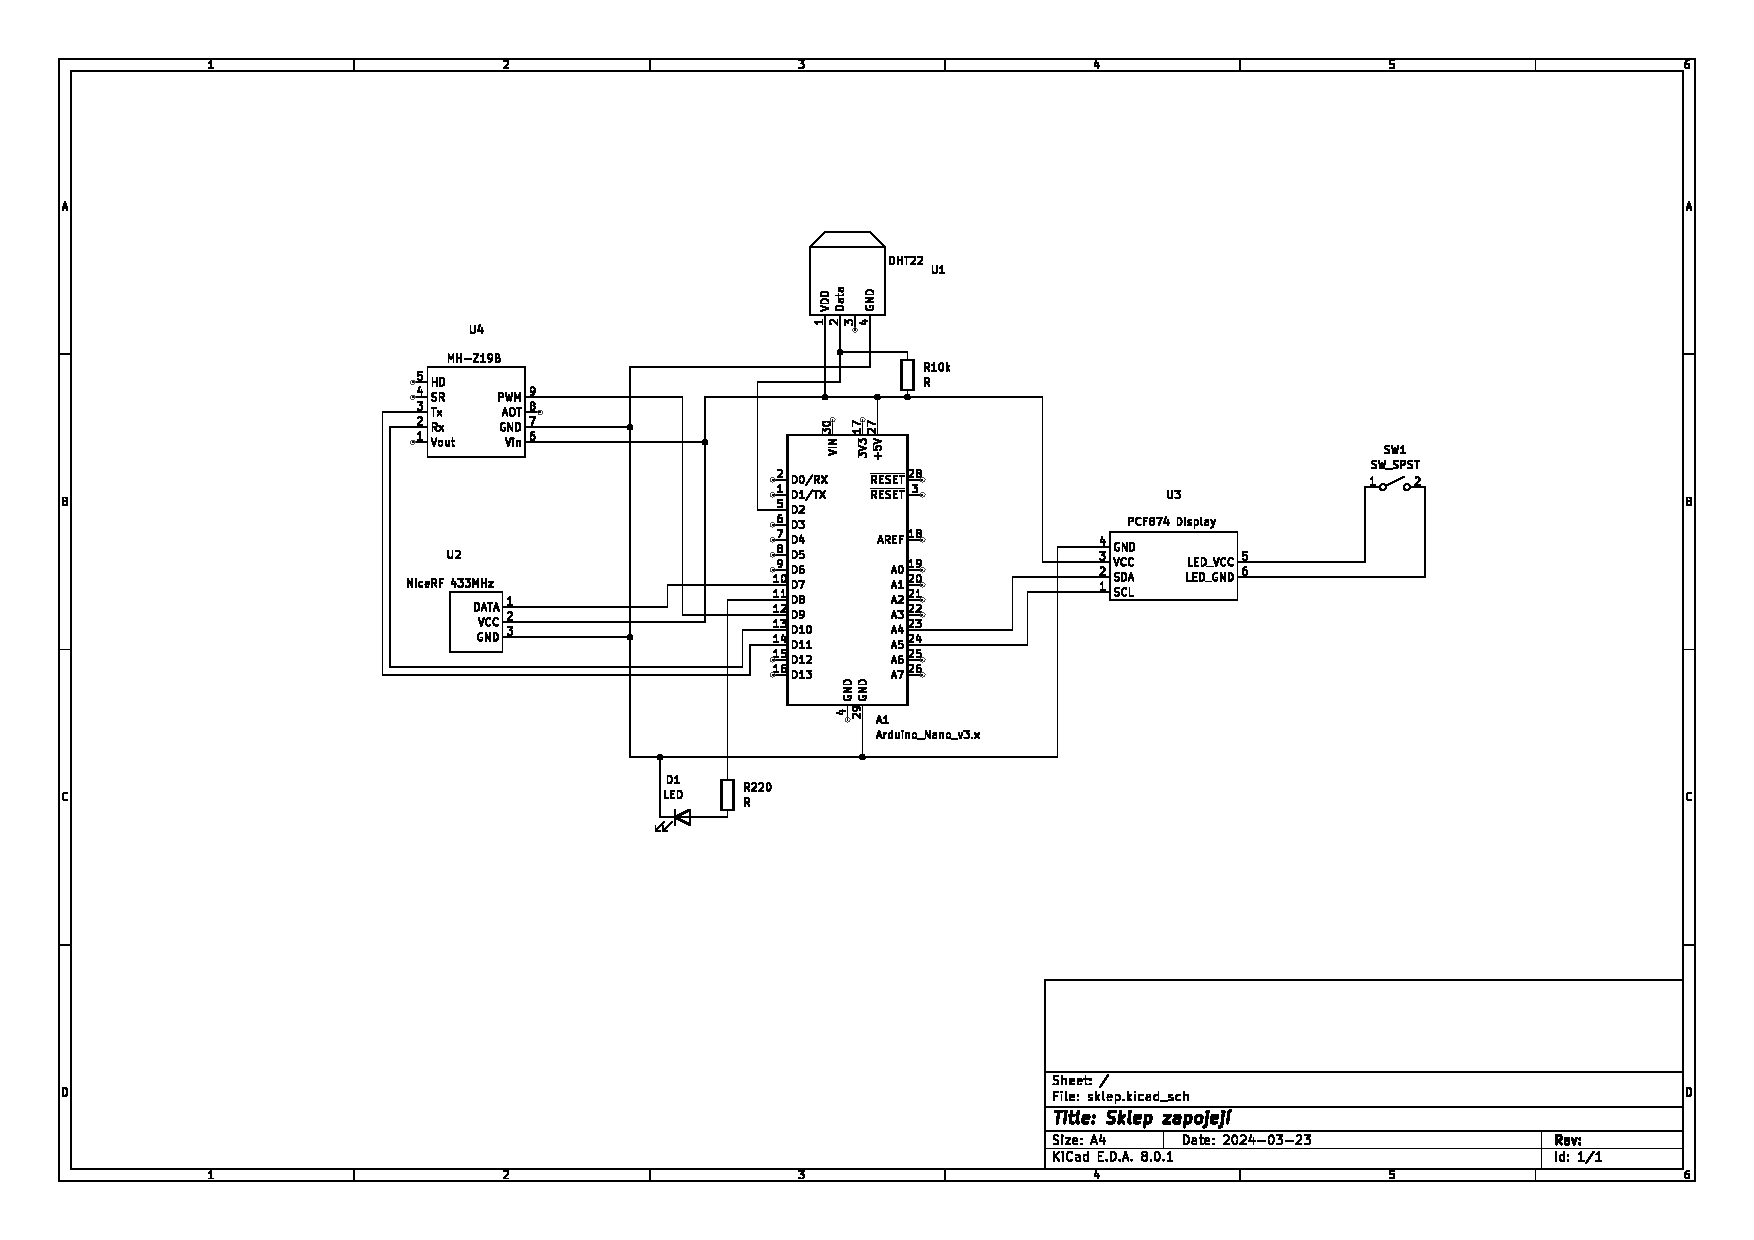
\includepdf[pages=-]{schemata/sklep_zapojeni.pdf}
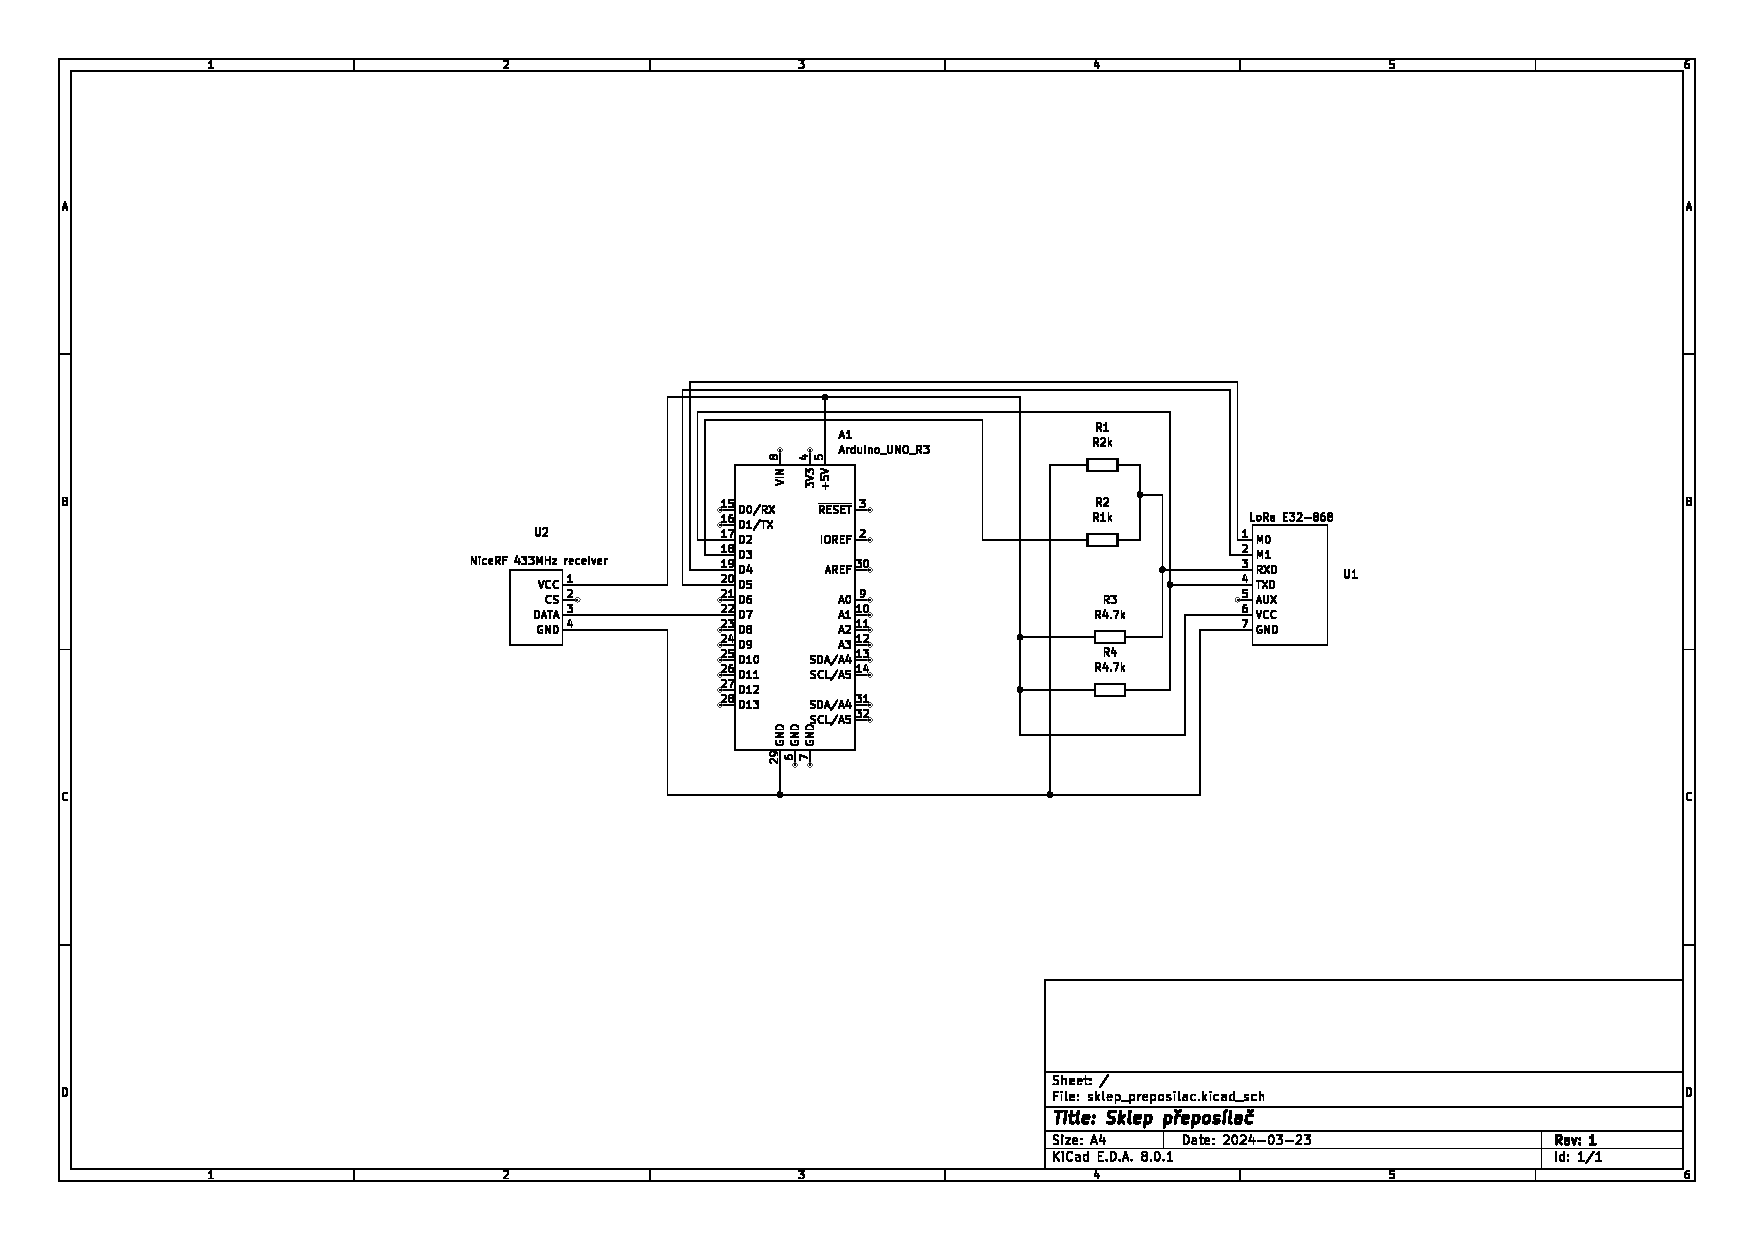
\includepdf[pages=-]{schemata/sklep_preposilac.pdf}
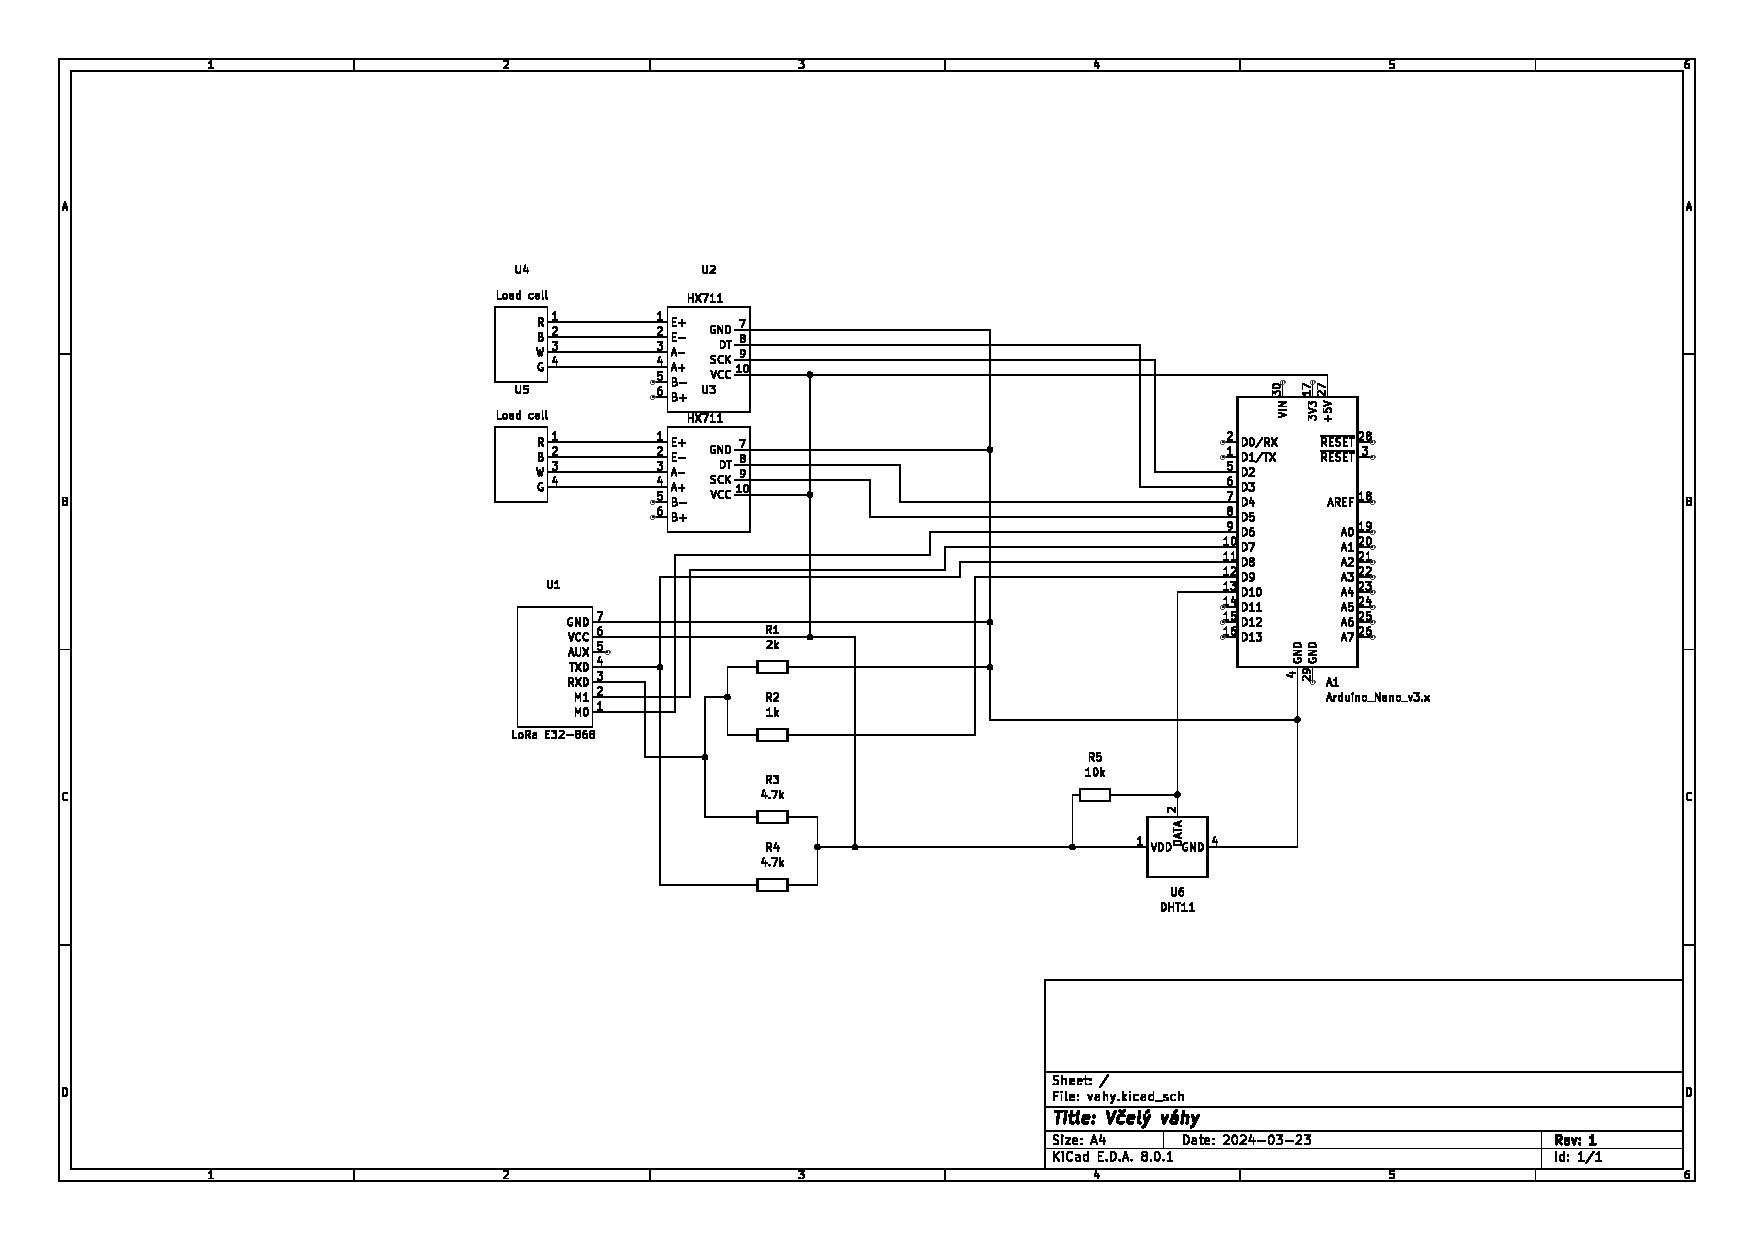
\includepdf[pages=-]{schemata/vahy.pdf}


% ============================================================================ %
 % Prilohy


% ============================================================================ %

\end{document}

% ============================================================================ %
